% APPENDIX
\chapter{Fit Plots of $M_{e\gamma}$}
\label{sec:EtogammaFitPlots}

Fit results of electron-photon invariant mass $M_{e\gamma}$ for the $e \rightarrow \gamma$ data-driven estimation in the electron channel. The procedure of the background estimation is described in Ch.~\ref{sec:BackgroundSubtraction_etog}.

The number of $e\righarrow\gamma$ events in data under the $Z$-peak $N_{MC-Zpeak}^{e\rightarrow\gamma}$ is extracted from the fit of the model: 
\begin{equation}
F_{fit}^{e\rightarrow\gamma} = N_{e\rightarrow\gamma} \cdot (RooNDKeysPdf \ast Gaussian) +  N_{other} \cdot (RooCMSShapePdf).
\end{equation}
\noindent{The function $RooNDKeysPdf$ is part of the RooFit package~\cite{ref_RooFit} and the $RooCMSShapePdf$ was developed specifically for CMS~\cite{ref_RooCMSShapePdf}. }

$F_{fit}^{e\rightarrow\gamma}$ has eight fit parameters. ``Nsig'' and ``Nbkg'' is the plots are $N_{e\rightarrow\gamma}$ and $N_{other}$, respectively, ``mean\_gau'' and ``sigma\_gau'' are parameters of the Gaussian distribution, ``CMS\_alpha'' and ``CMS\_beta'' are parameters of the exponential component of the $RooCMSShapePdf$, and ``CMS\_gamma'' and ``CMS\_peak'' are parameters of the turn over component of the $RooCMSShapePdf$.  

\begin{figure}[htb]
  \begin{center}
   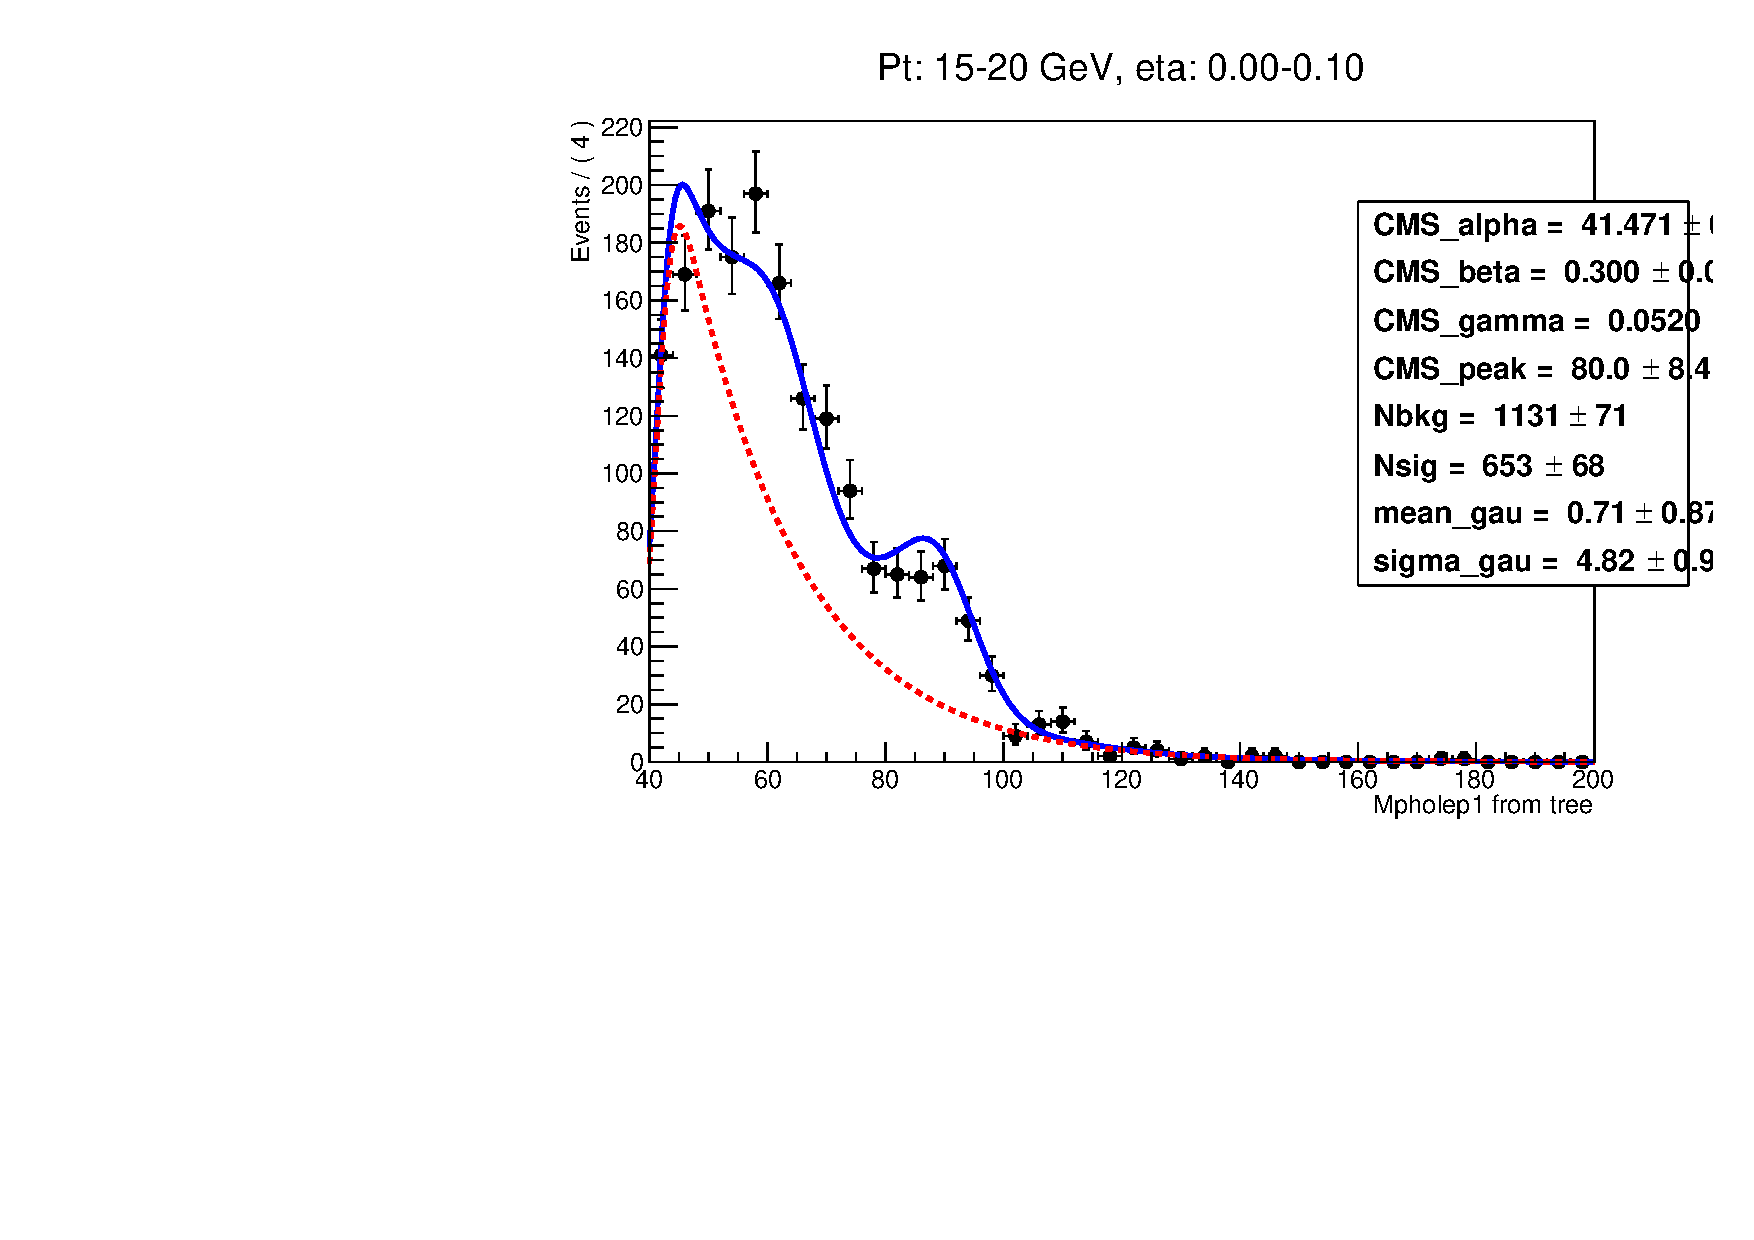
\includegraphics[width=0.45\textwidth]{../figs/figs_v11/ELECTRON_WGamma/EtoGammaFits/sa_hZmass_h_Data_EtoGamma_Enr_BARREL_pt15to20_ieta0.pdf}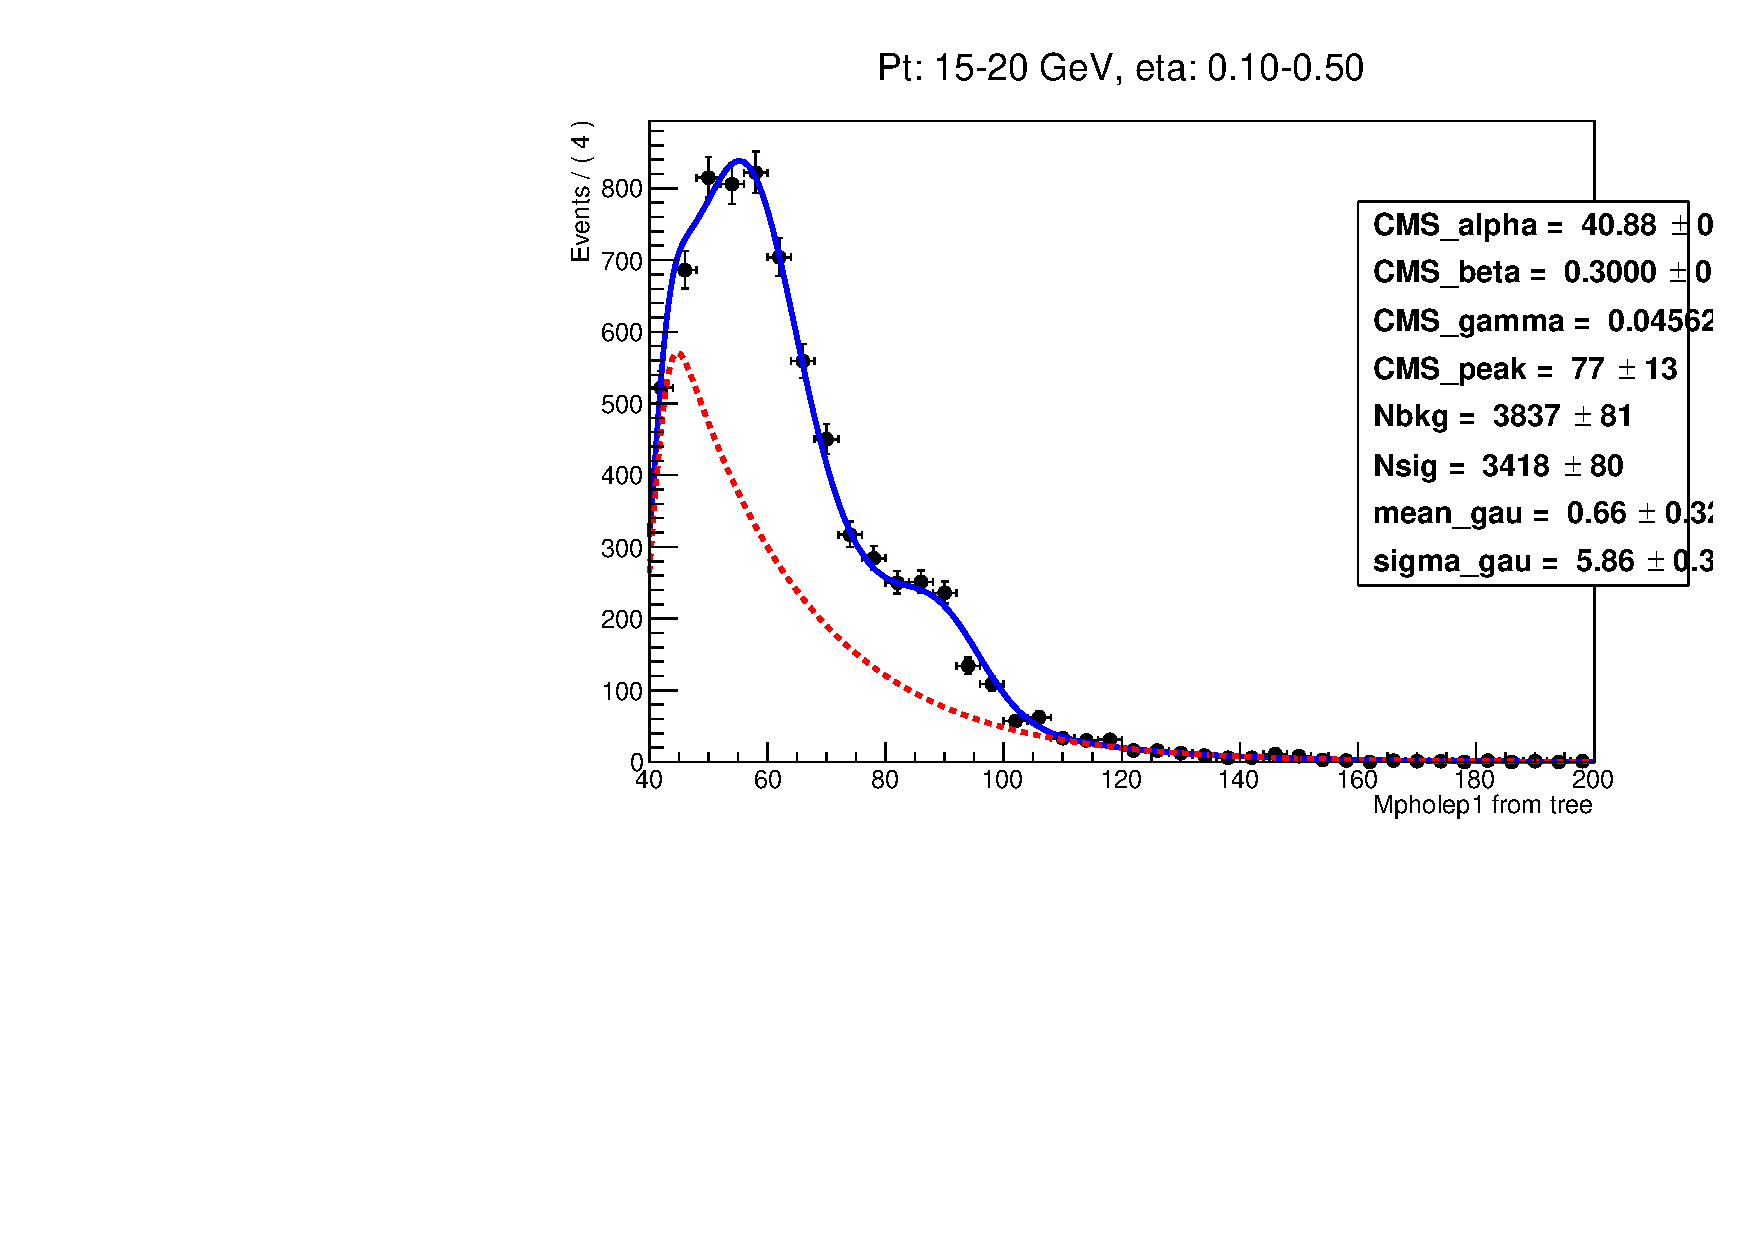
\includegraphics[width=0.45\textwidth]{../figs/figs_v11/ELECTRON_WGamma/EtoGammaFits/sa_hZmass_h_Data_EtoGamma_Enr_BARREL_pt15to20_ieta1.pdf}\\
   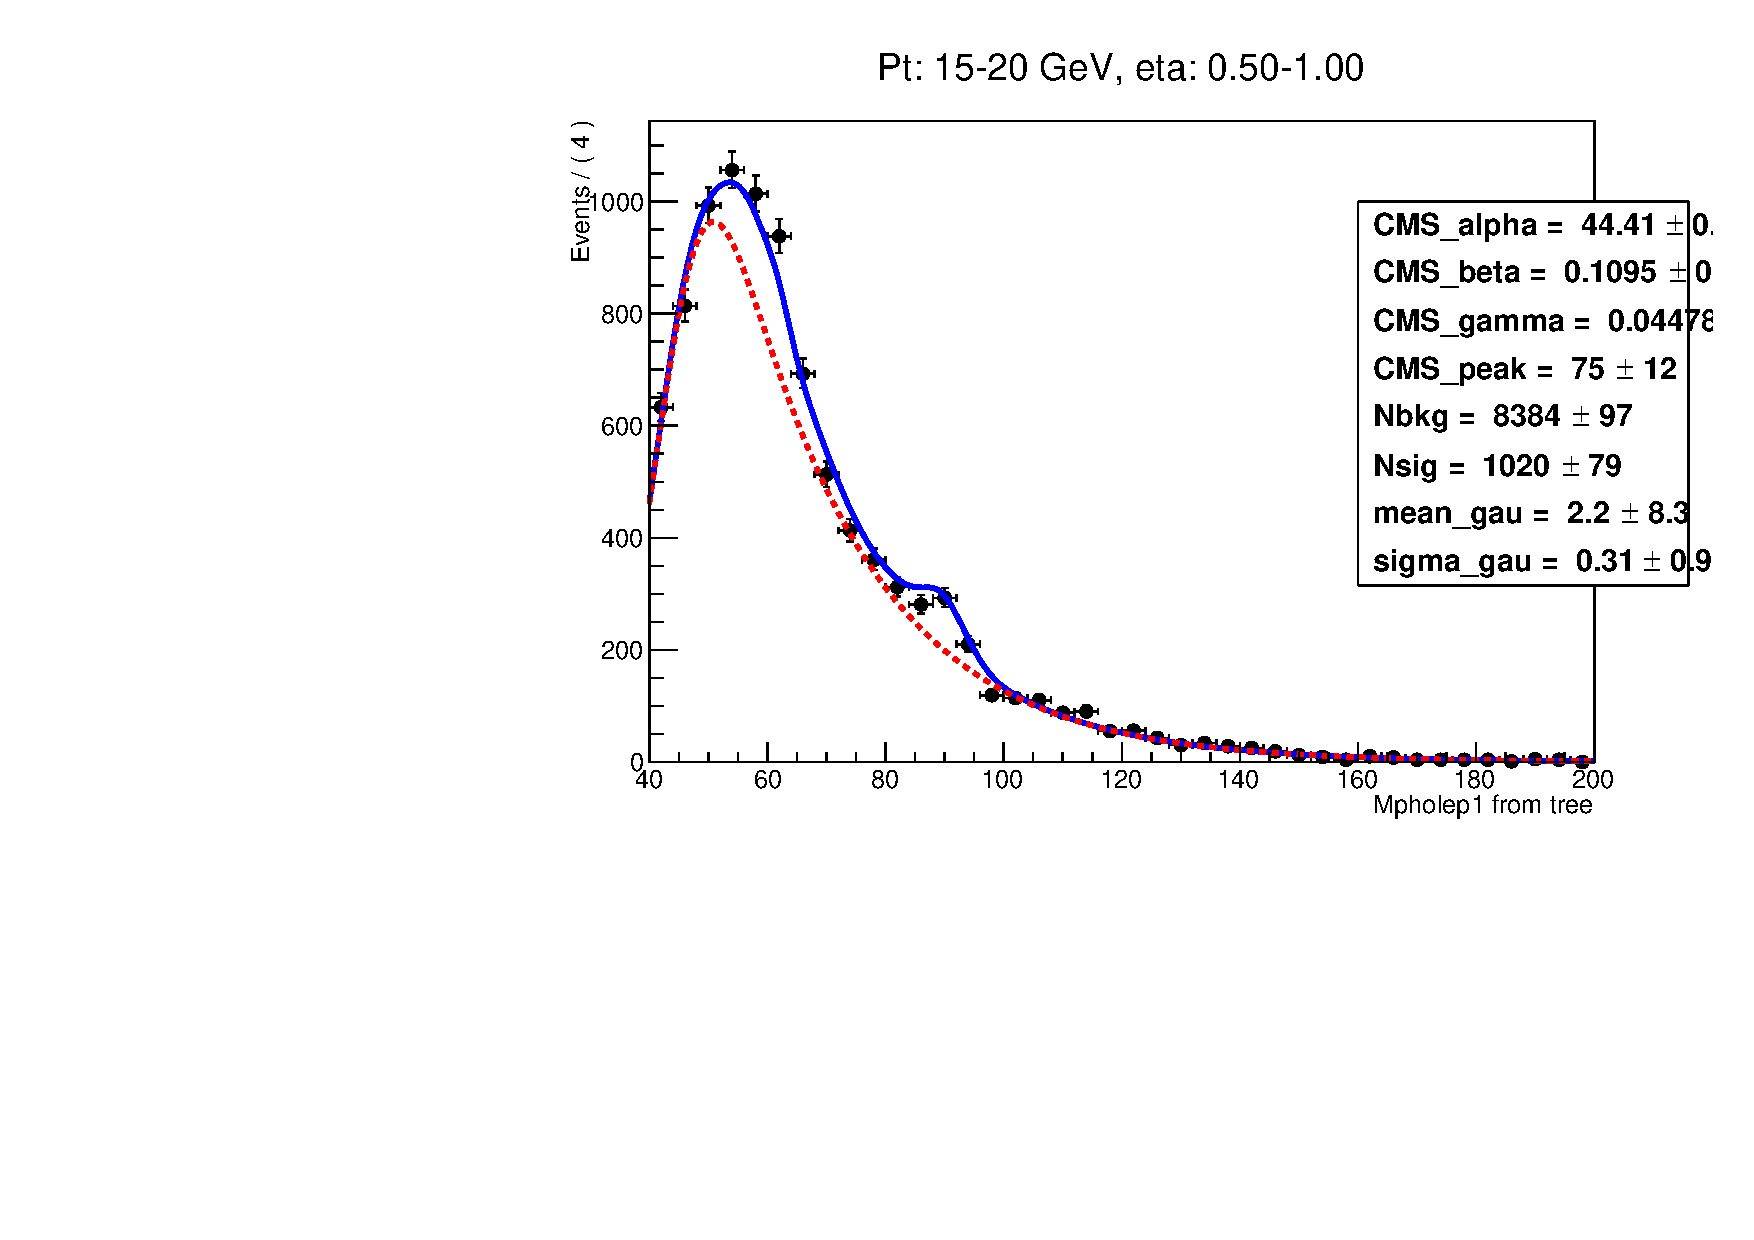
\includegraphics[width=0.45\textwidth]{../figs/figs_v11/ELECTRON_WGamma/EtoGammaFits/sa_hZmass_h_Data_EtoGamma_Enr_BARREL_pt15to20_ieta2.pdf}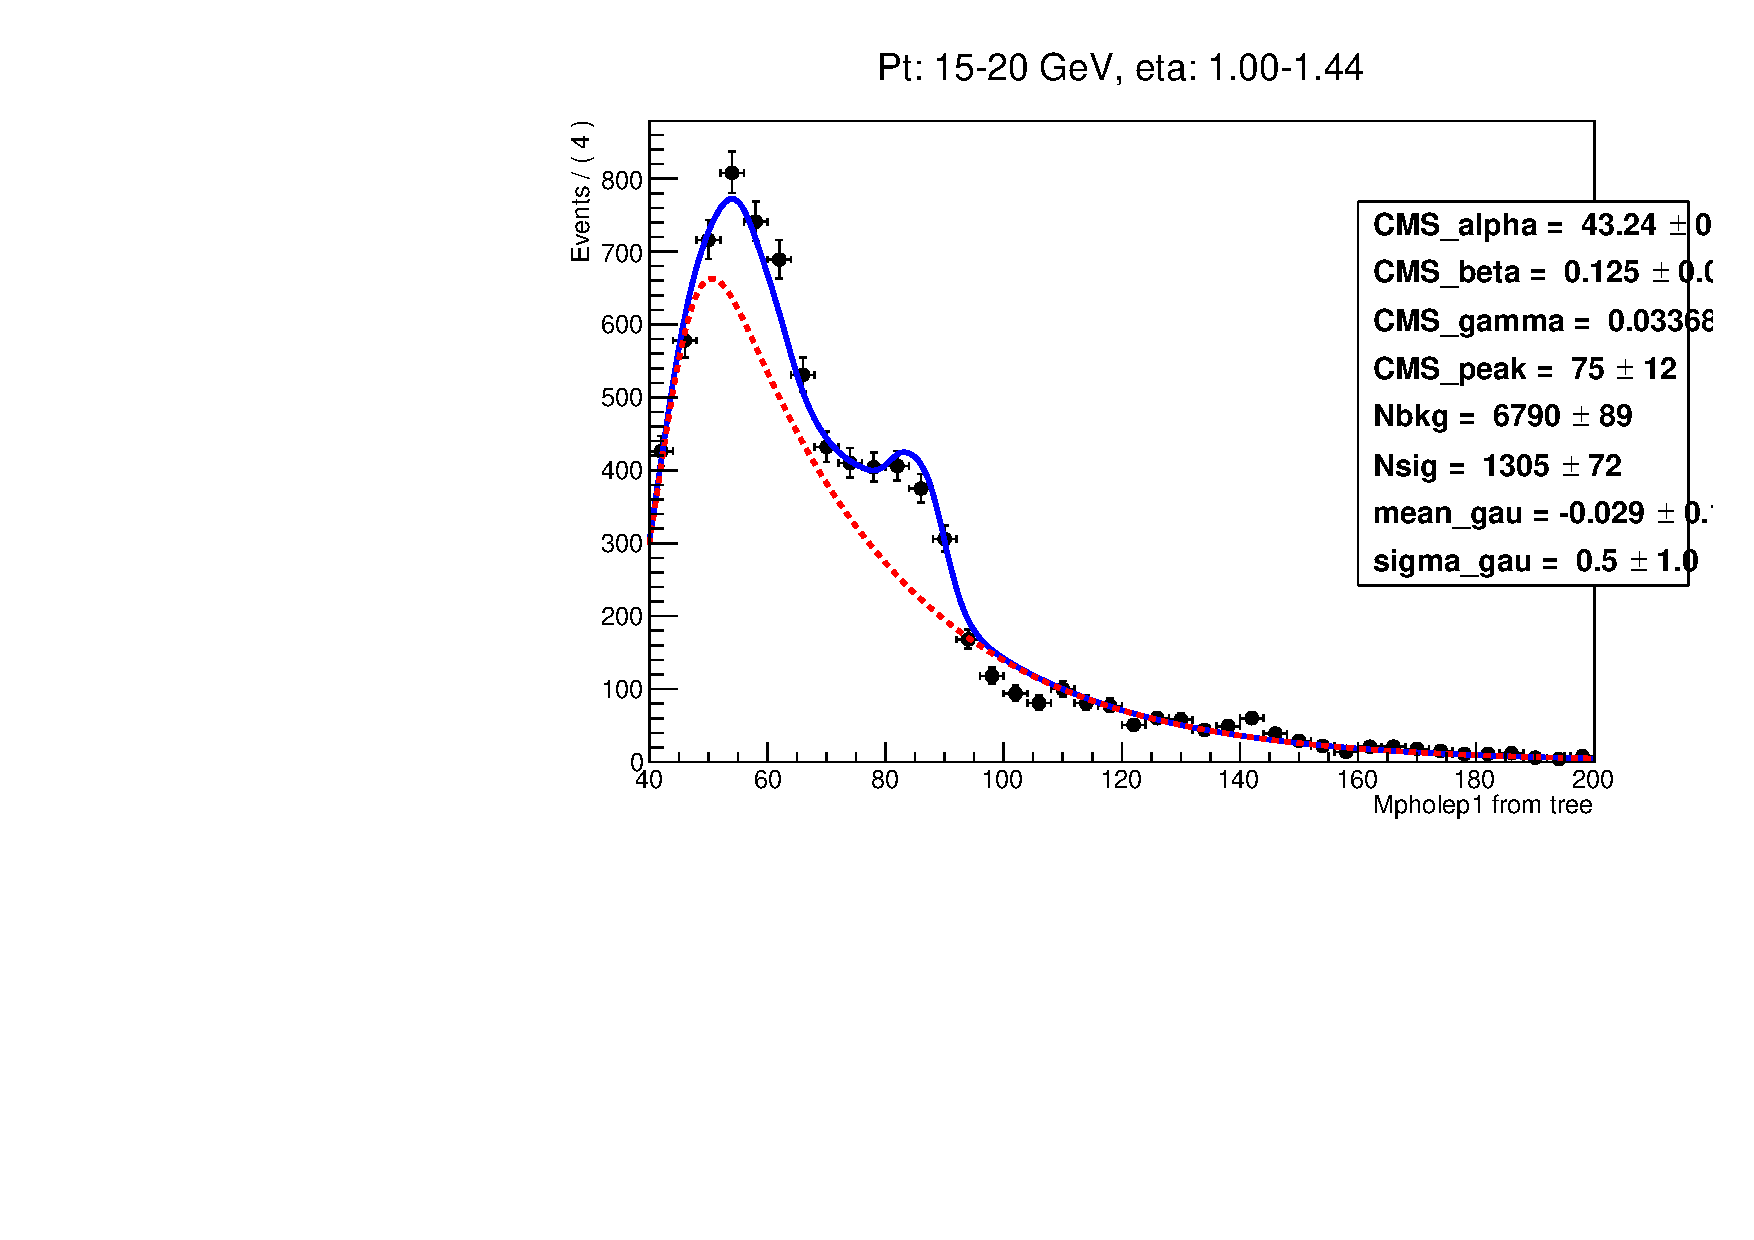
\includegraphics[width=0.45\textwidth]{../figs/figs_v11/ELECTRON_WGamma/EtoGammaFits/sa_hZmass_h_Data_EtoGamma_Enr_BARREL_pt15to20_ieta3.pdf}\\
   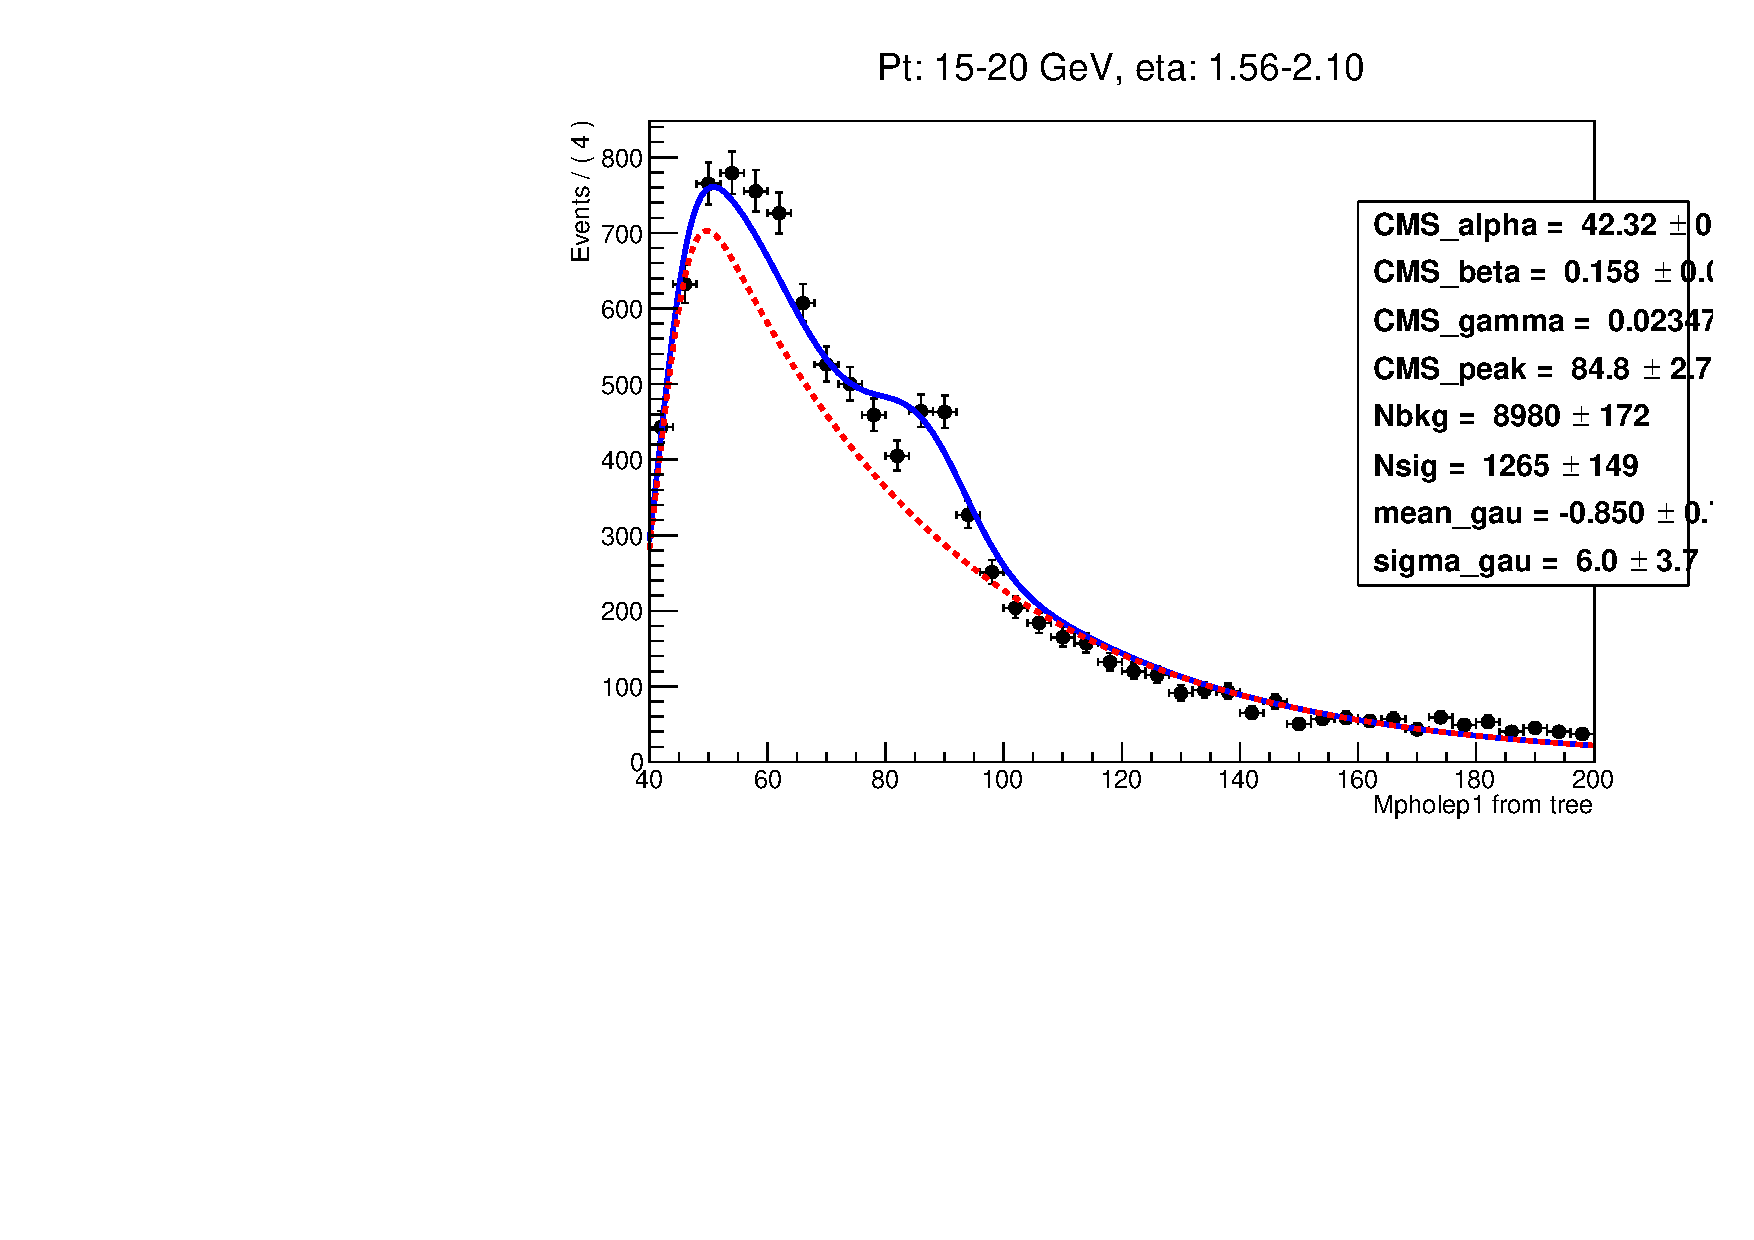
\includegraphics[width=0.45\textwidth]{../figs/figs_v11/ELECTRON_WGamma/EtoGammaFits/sa_hZmass_h_Data_EtoGamma_Enr_ENDCAP_pt15to20_ieta0.pdf}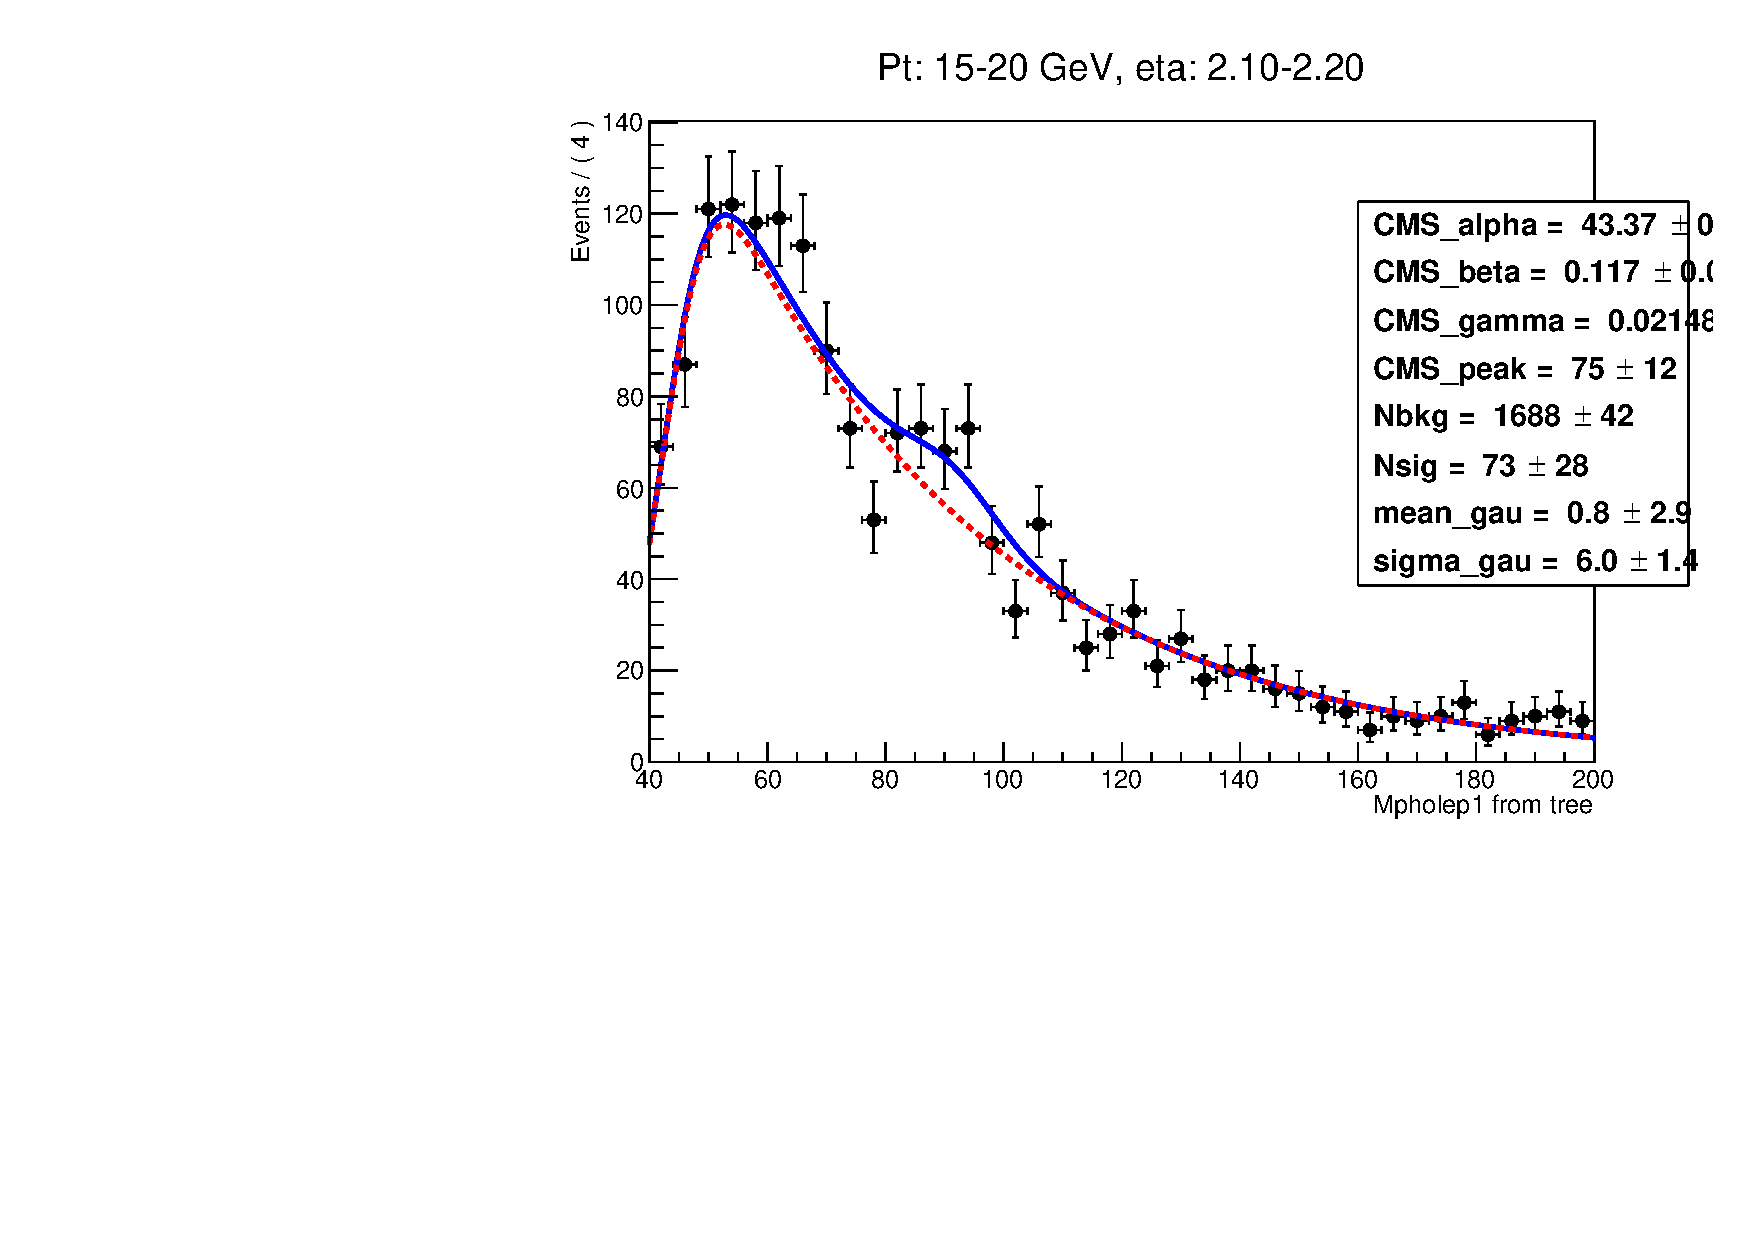
\includegraphics[width=0.45\textwidth]{../figs/figs_v11/ELECTRON_WGamma/EtoGammaFits/sa_hZmass_h_Data_EtoGamma_Enr_ENDCAP_pt15to20_ieta1.pdf}\\
   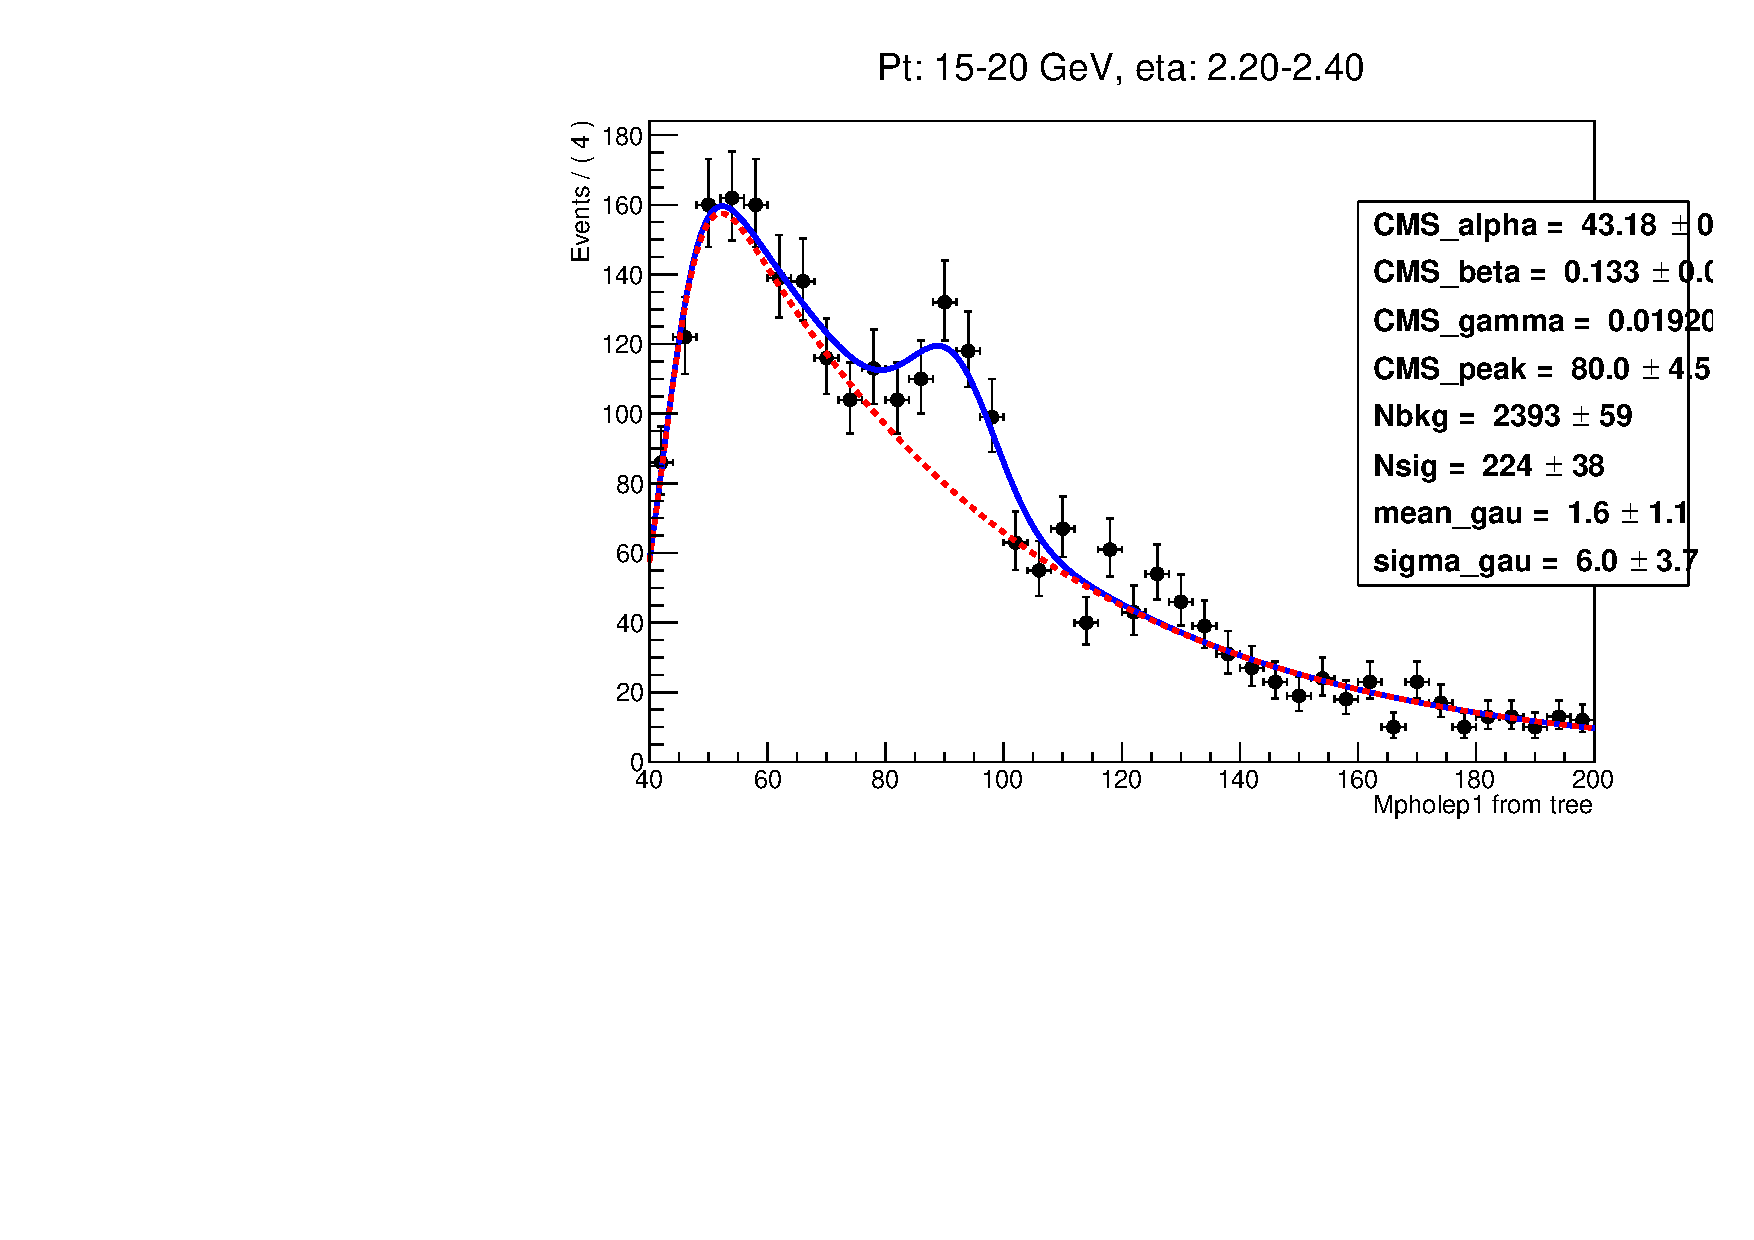
\includegraphics[width=0.45\textwidth]{../figs/figs_v11/ELECTRON_WGamma/EtoGammaFits/sa_hZmass_h_Data_EtoGamma_Enr_ENDCAP_pt15to20_ieta2.pdf}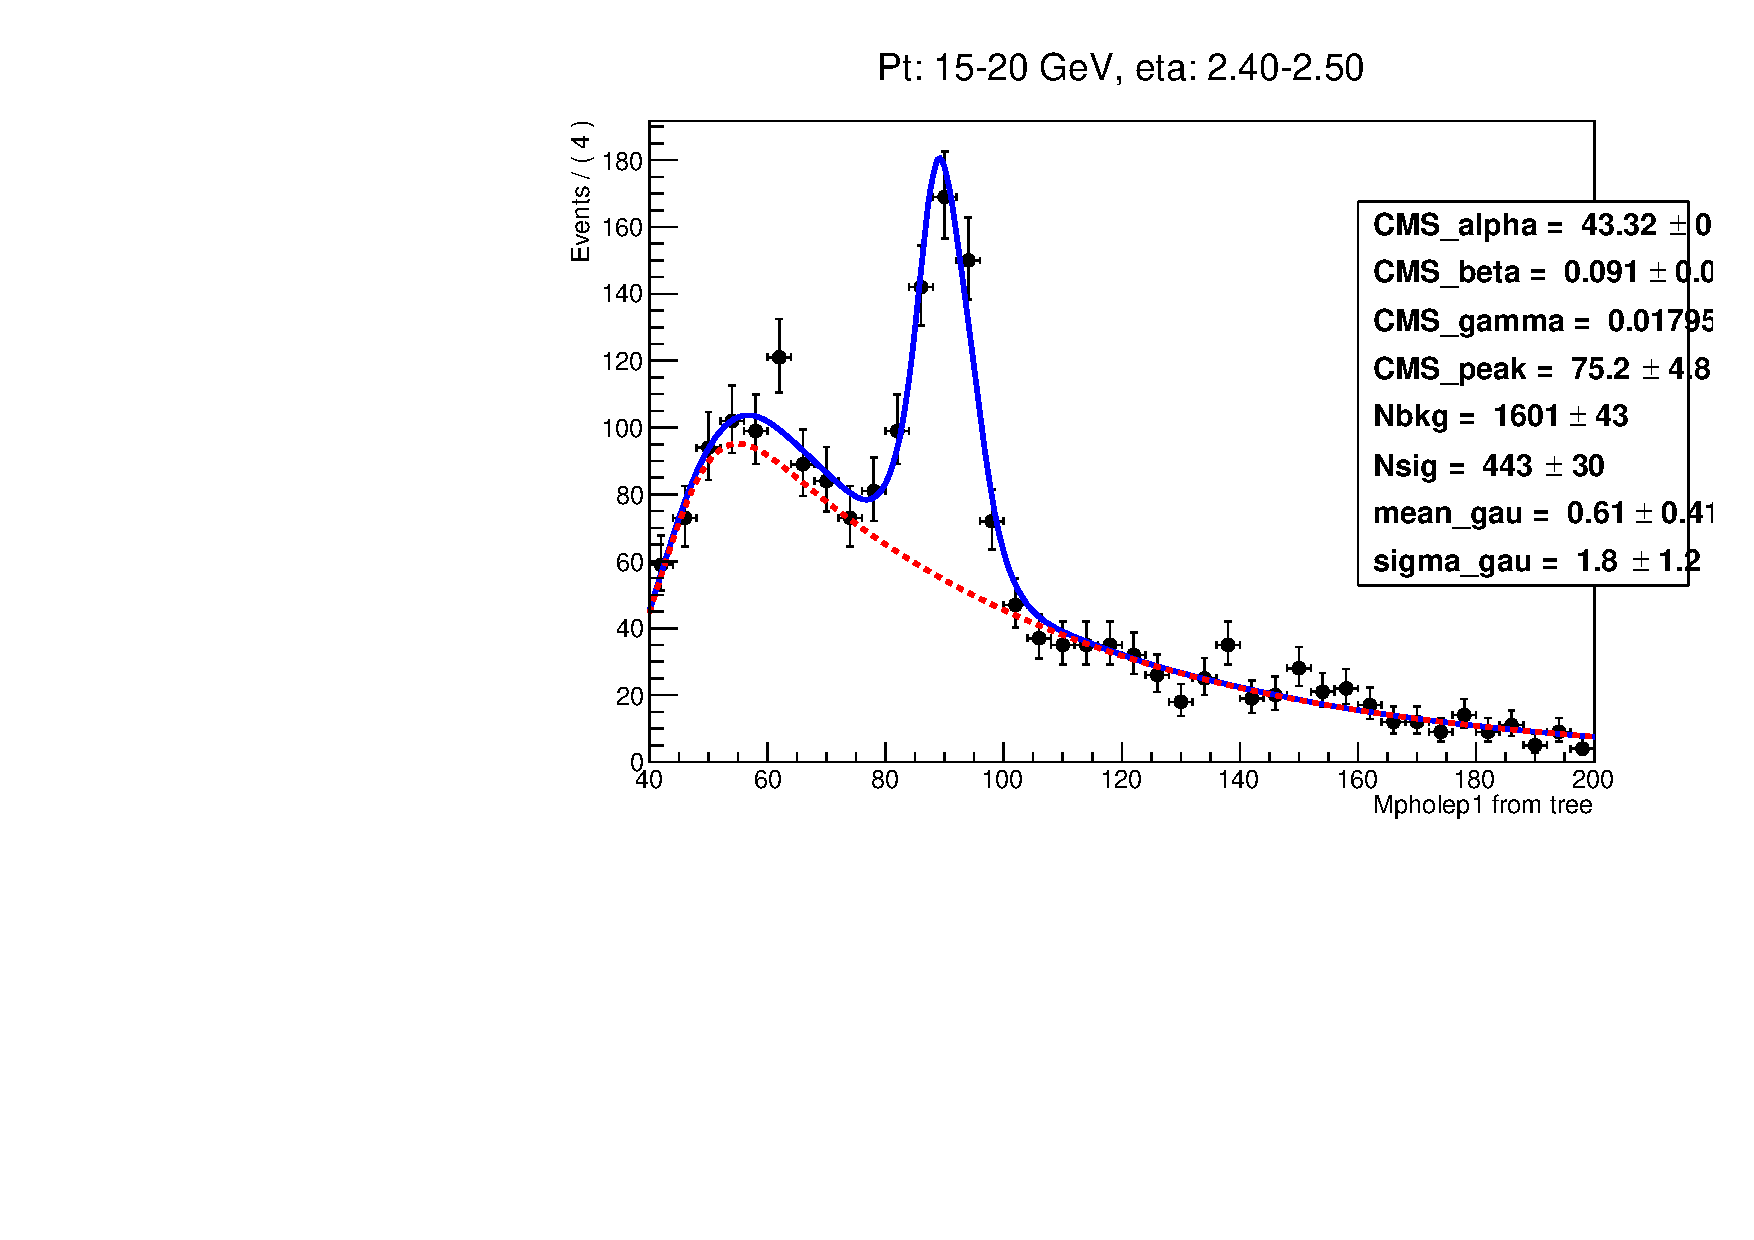
\includegraphics[width=0.45\textwidth]{../figs/figs_v11/ELECTRON_WGamma/EtoGammaFits/sa_hZmass_h_Data_EtoGamma_Enr_ENDCAP_pt15to20_ieta3.pdf}\\
  \label{fig:etogFits_15to20}
  \caption{$M_{e\gamma}$ fits, $W\gamma$, electron channel, 15-20 GeV, 8 $\eta^{\gamma}$ bins.}
  \end{center}
\end{figure}

\begin{figure}[htb]
  \begin{center}
   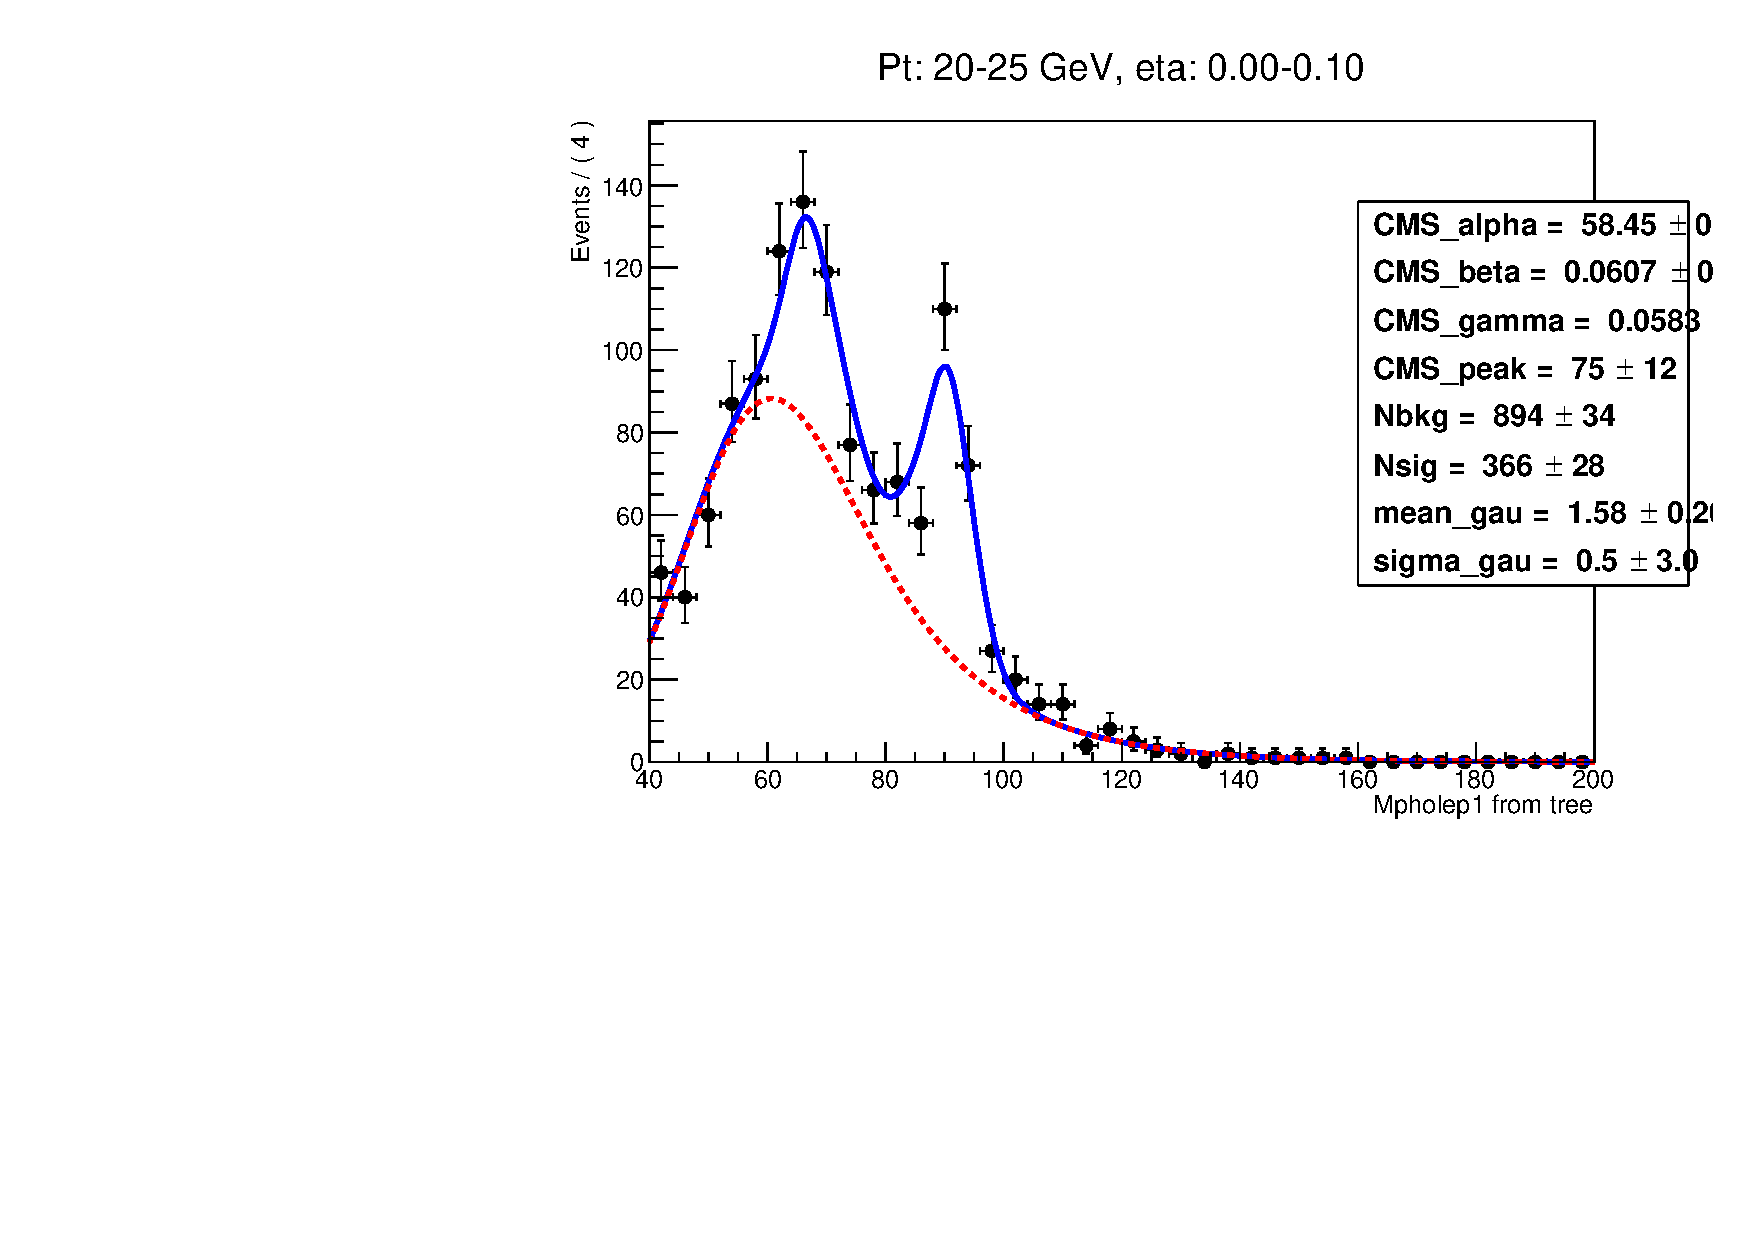
\includegraphics[width=0.45\textwidth]{../figs/figs_v11/ELECTRON_WGamma/EtoGammaFits/sa_hZmass_h_Data_EtoGamma_Enr_BARREL_pt20to25_ieta0.pdf}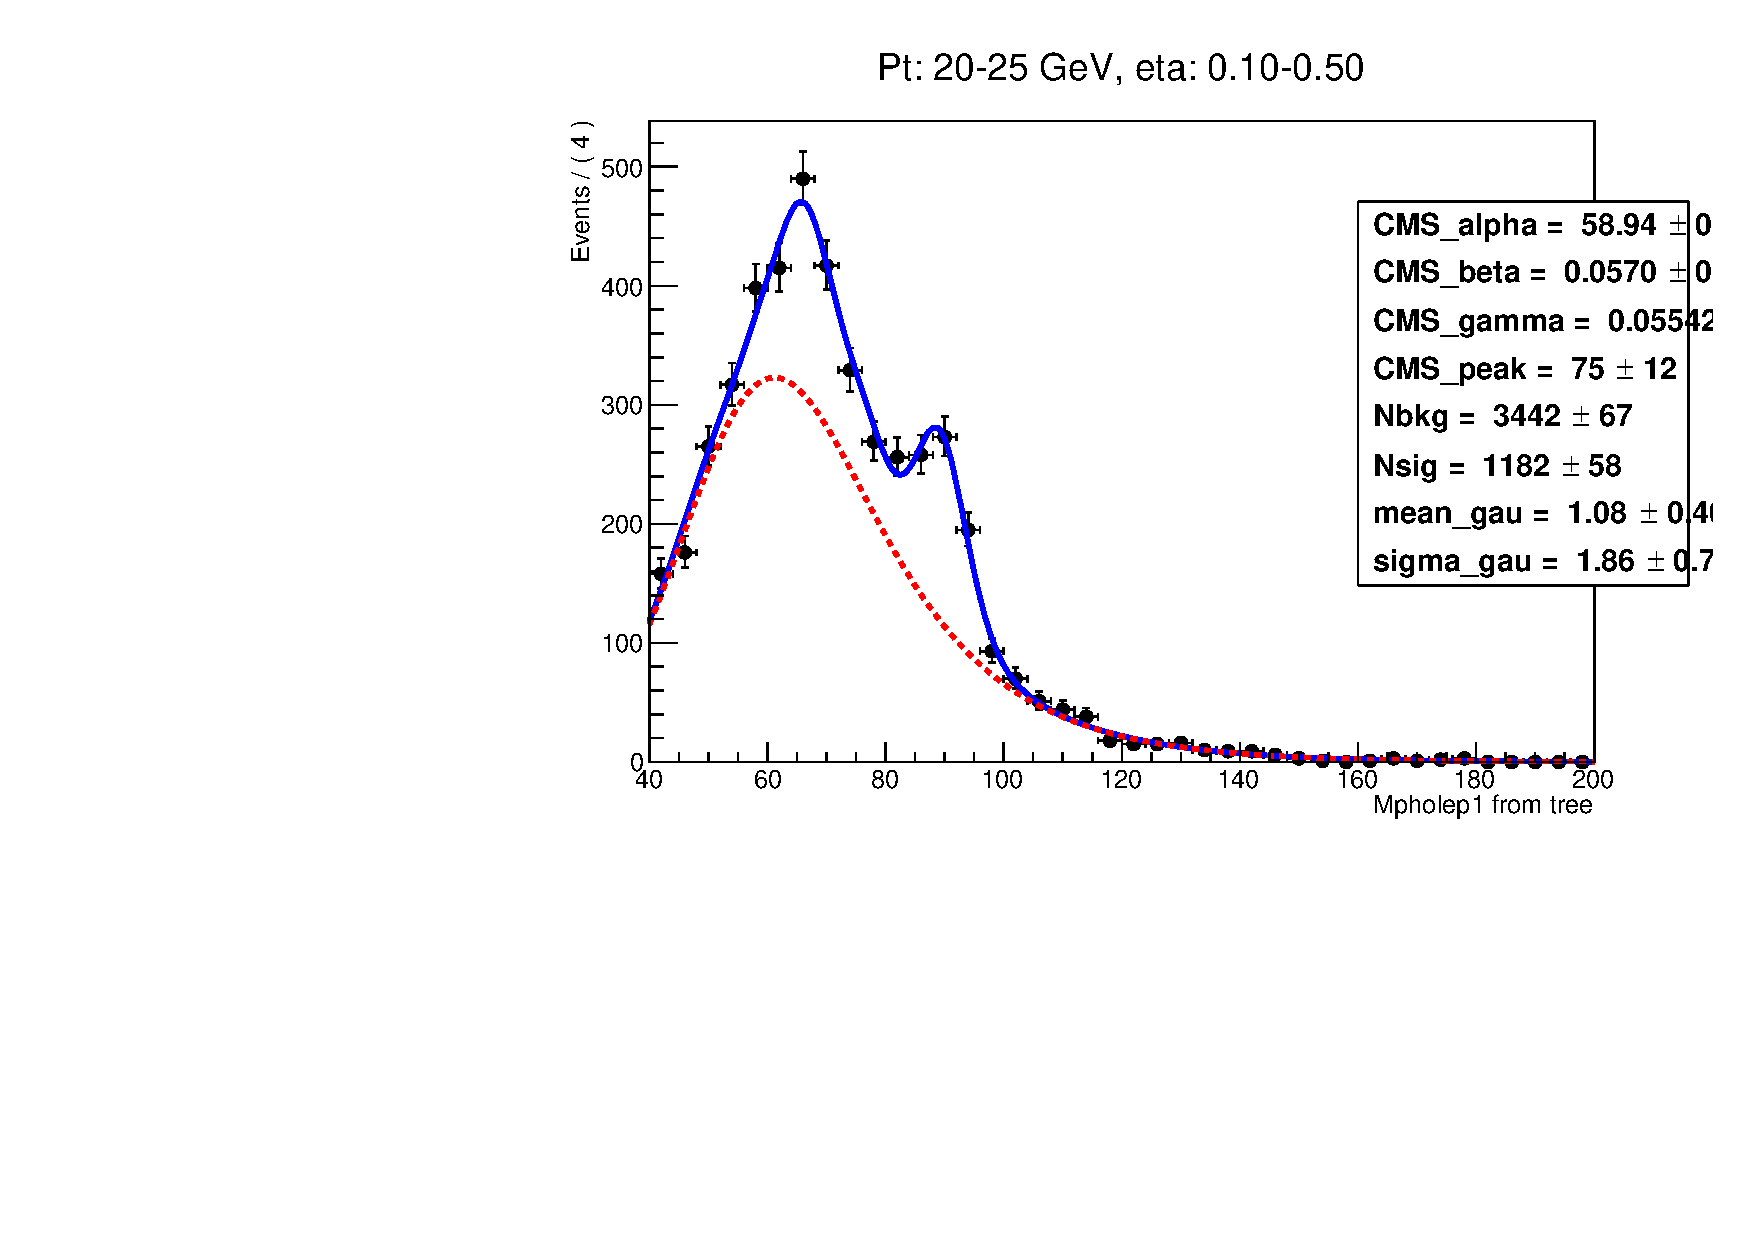
\includegraphics[width=0.45\textwidth]{../figs/figs_v11/ELECTRON_WGamma/EtoGammaFits/sa_hZmass_h_Data_EtoGamma_Enr_BARREL_pt20to25_ieta1.pdf}\\
   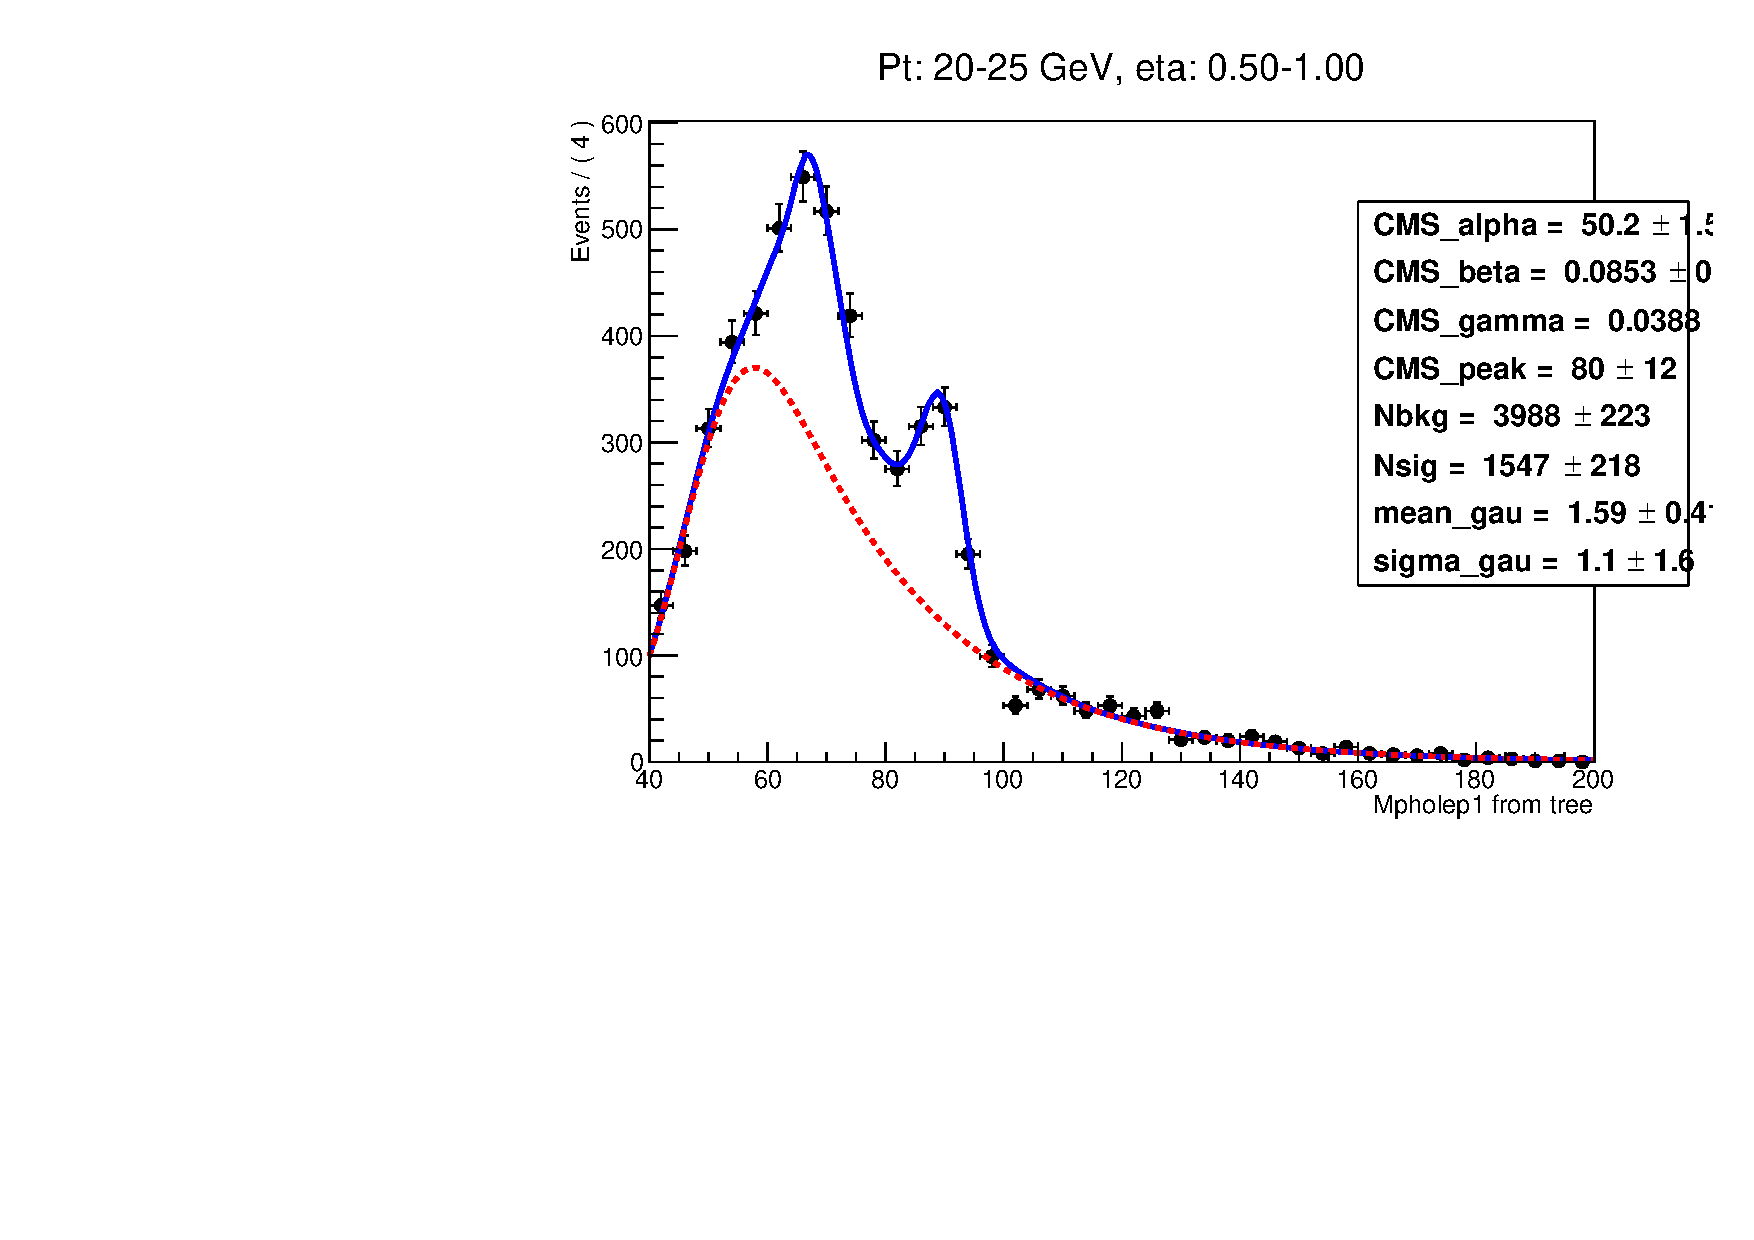
\includegraphics[width=0.45\textwidth]{../figs/figs_v11/ELECTRON_WGamma/EtoGammaFits/sa_hZmass_h_Data_EtoGamma_Enr_BARREL_pt20to25_ieta2.pdf}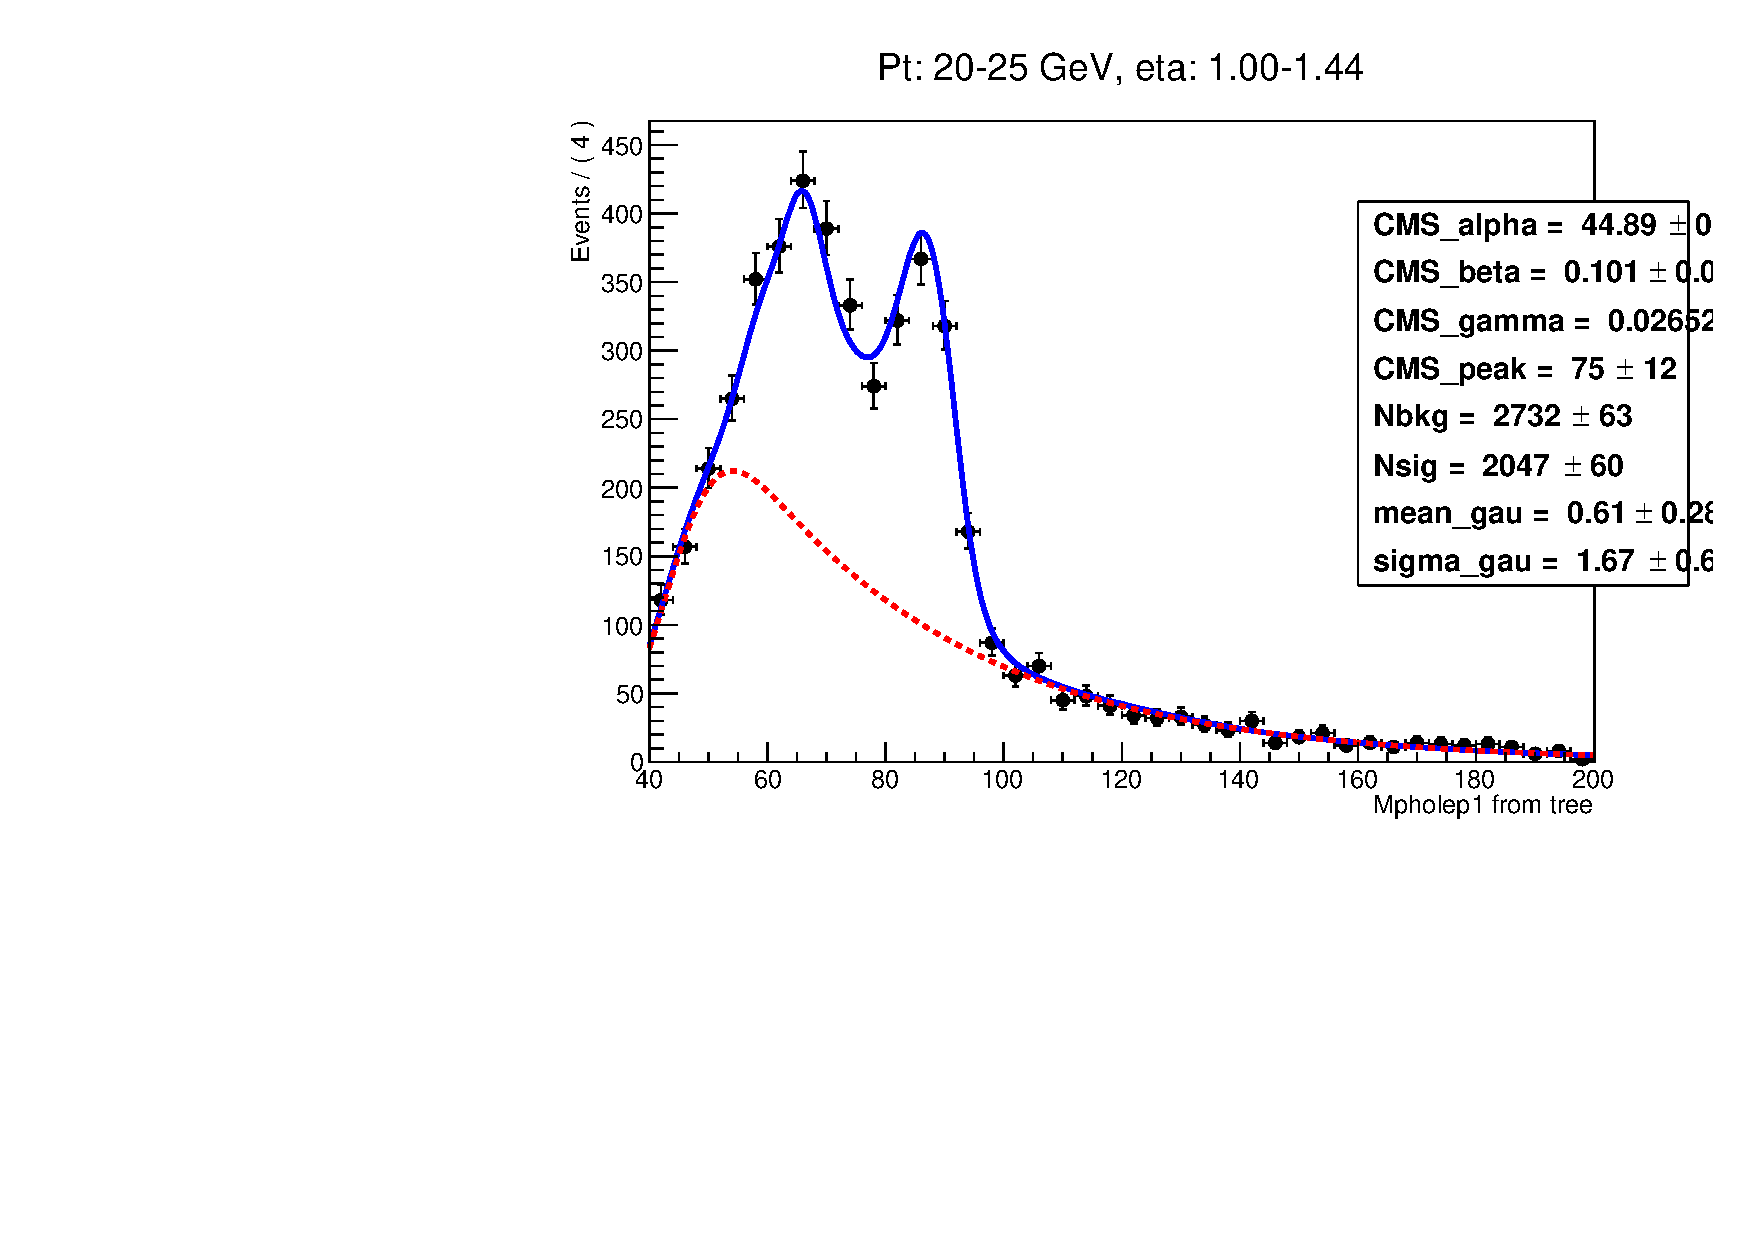
\includegraphics[width=0.45\textwidth]{../figs/figs_v11/ELECTRON_WGamma/EtoGammaFits/sa_hZmass_h_Data_EtoGamma_Enr_BARREL_pt20to25_ieta3.pdf}\\
   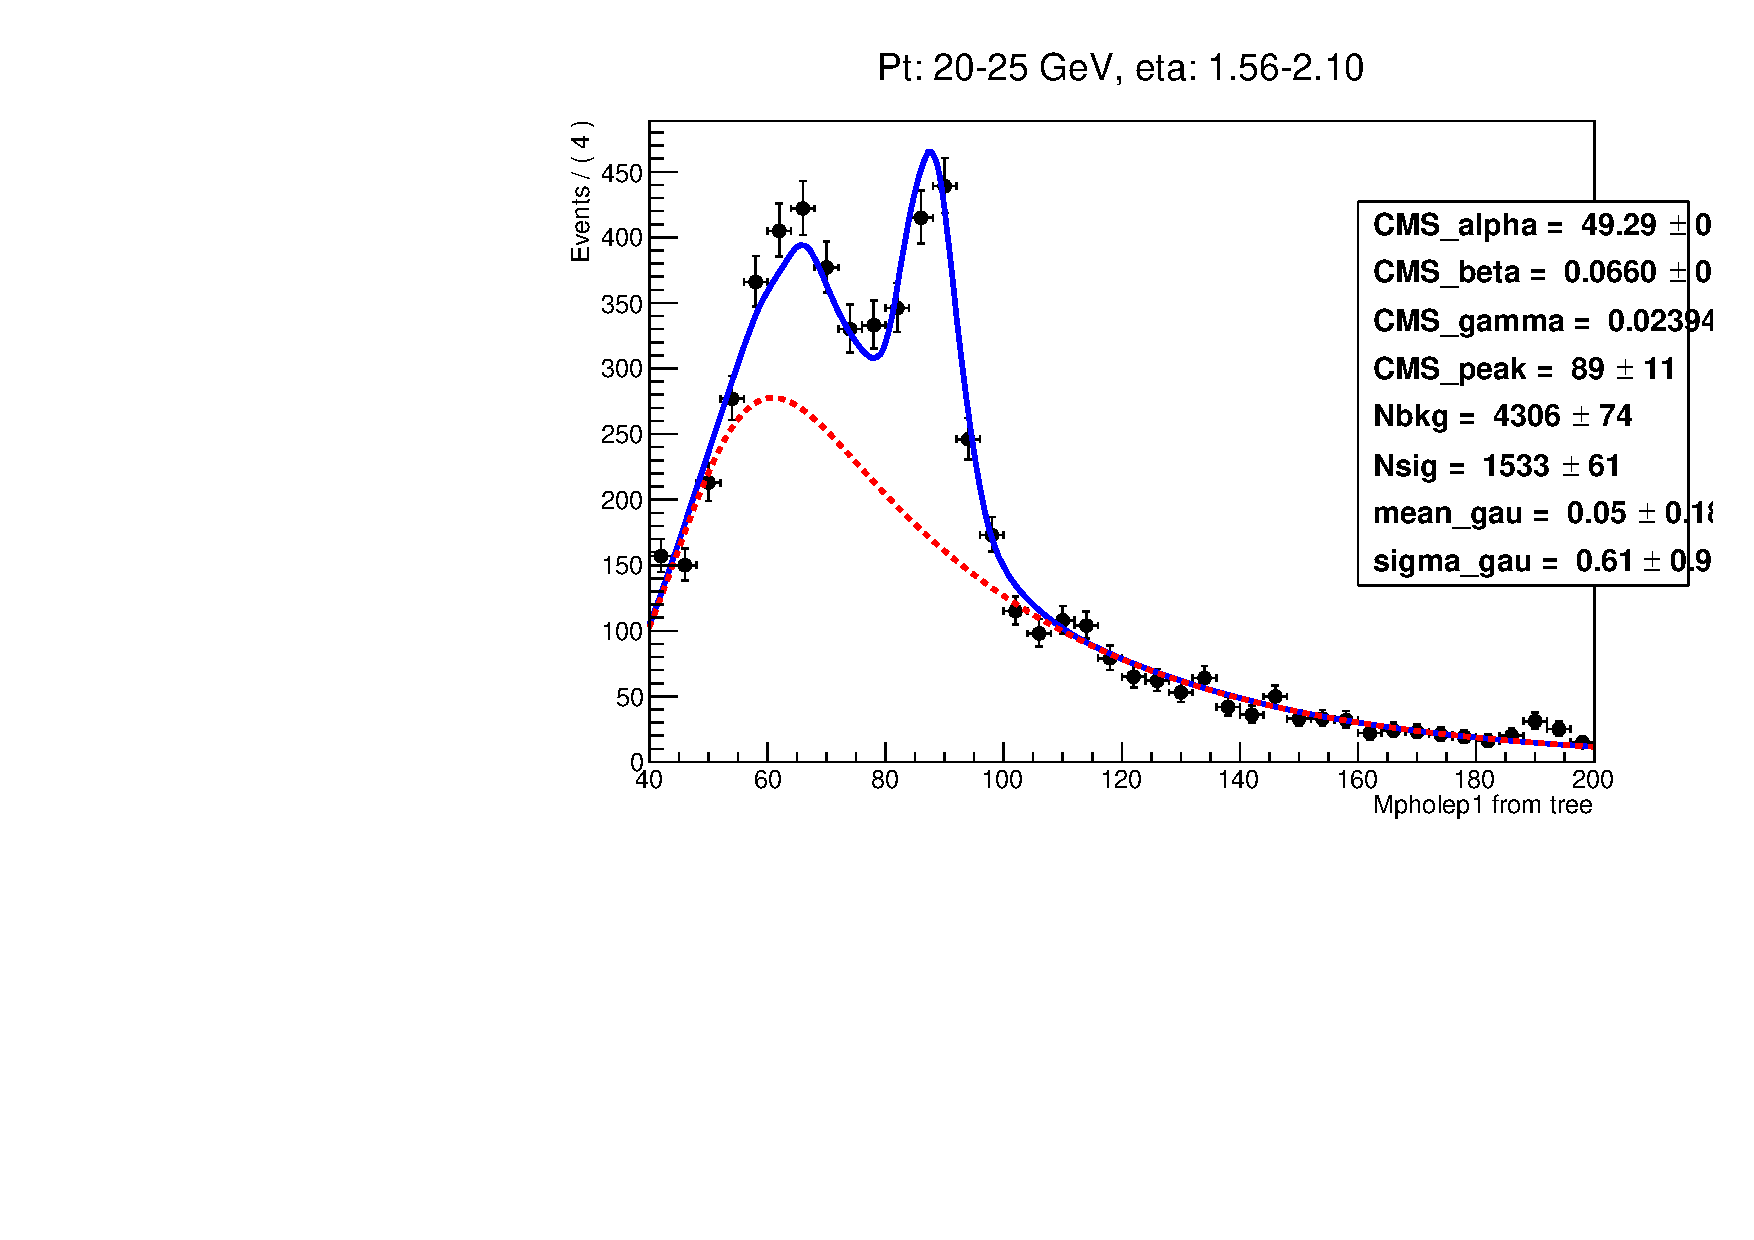
\includegraphics[width=0.45\textwidth]{../figs/figs_v11/ELECTRON_WGamma/EtoGammaFits/sa_hZmass_h_Data_EtoGamma_Enr_ENDCAP_pt20to25_ieta0.pdf}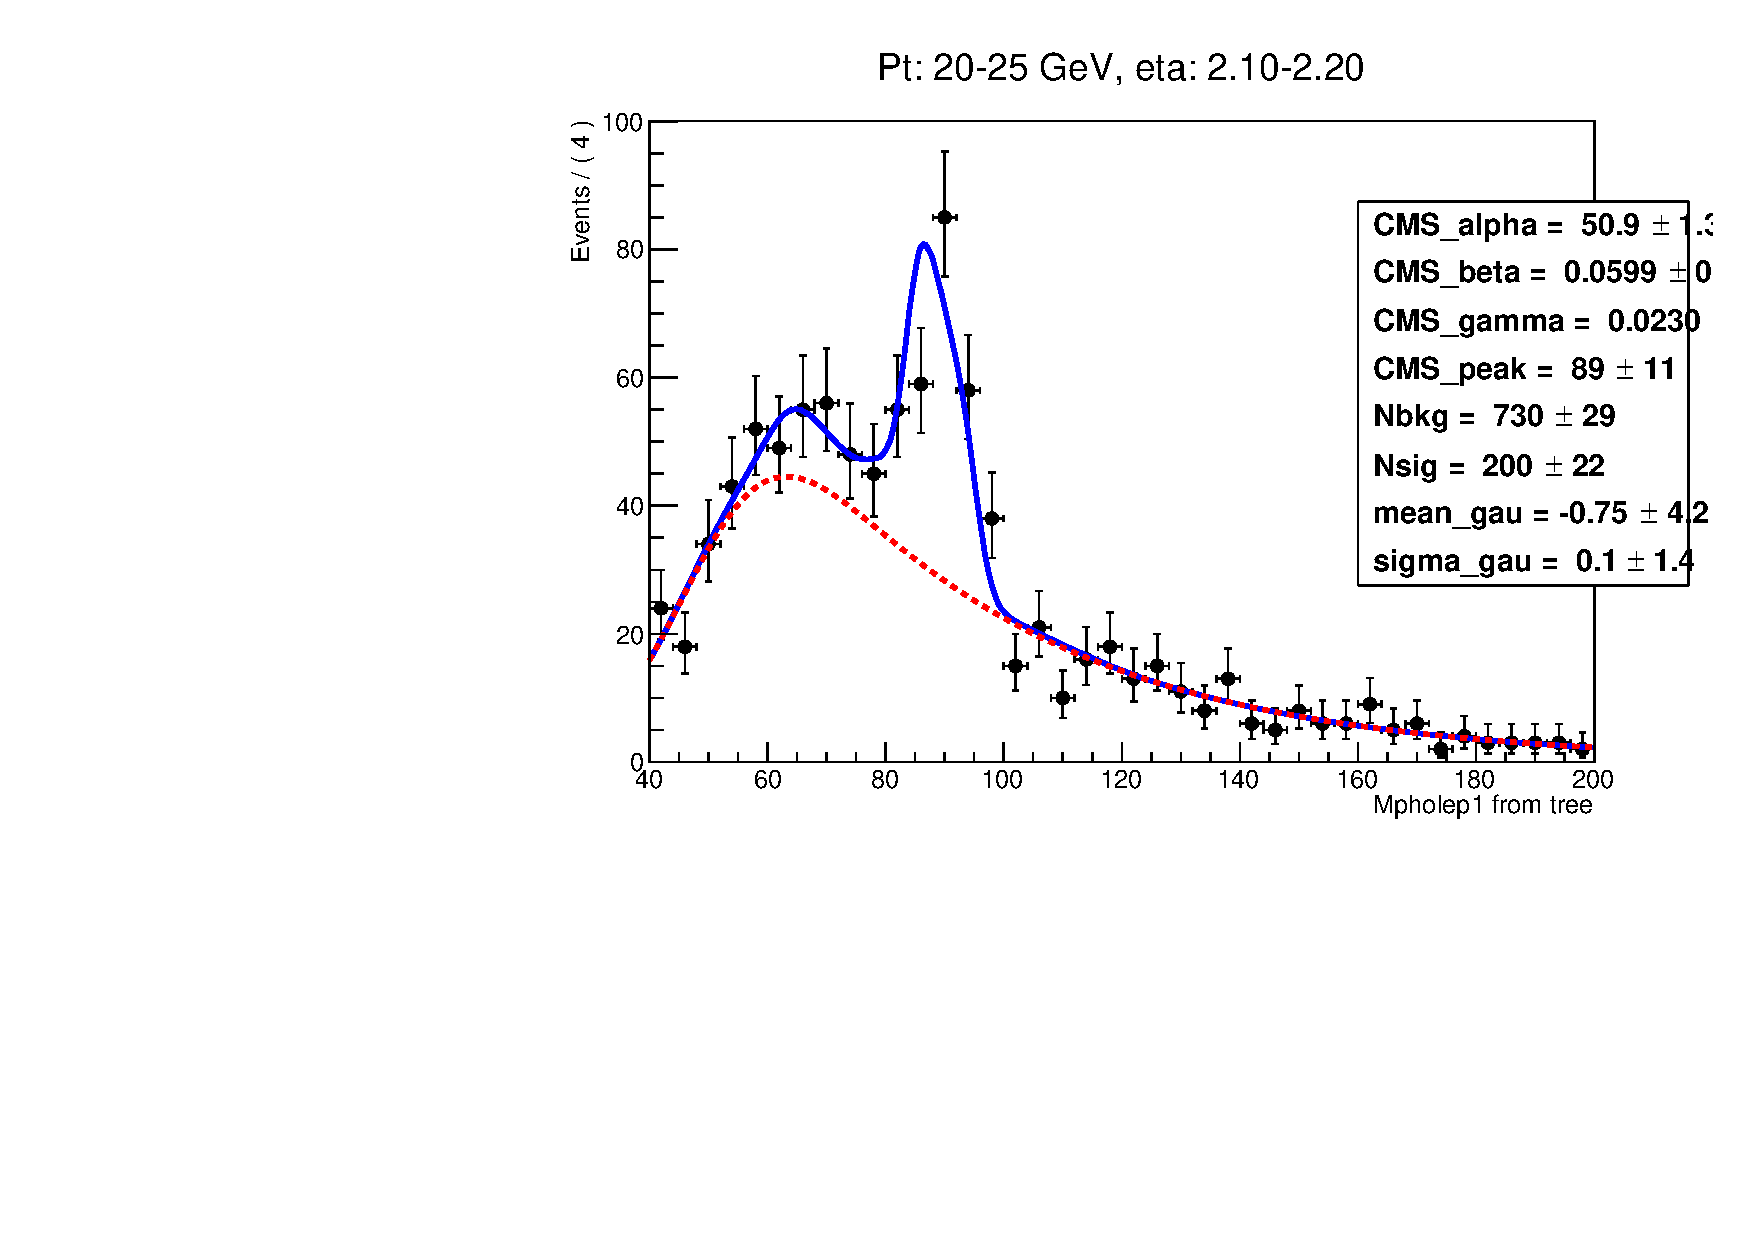
\includegraphics[width=0.45\textwidth]{../figs/figs_v11/ELECTRON_WGamma/EtoGammaFits/sa_hZmass_h_Data_EtoGamma_Enr_ENDCAP_pt20to25_ieta1.pdf}\\
   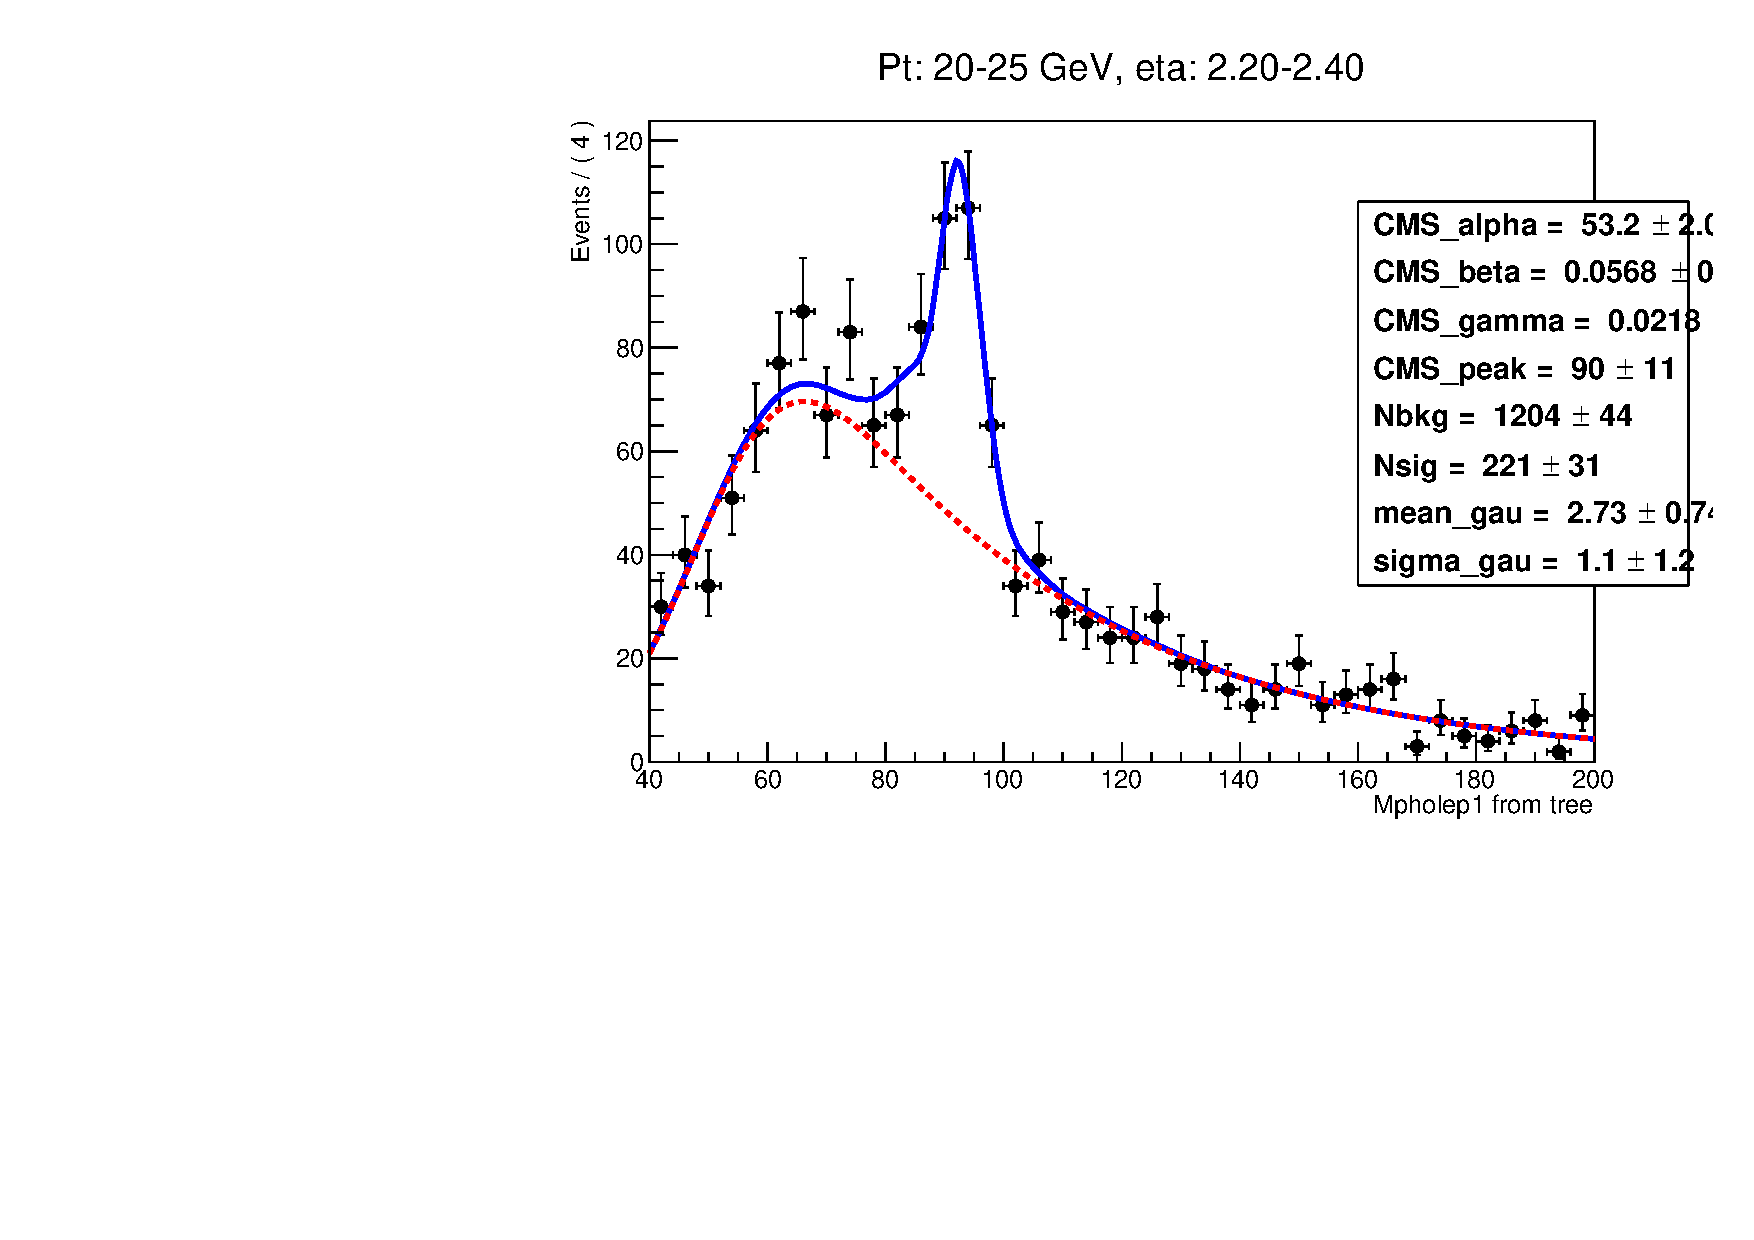
\includegraphics[width=0.45\textwidth]{../figs/figs_v11/ELECTRON_WGamma/EtoGammaFits/sa_hZmass_h_Data_EtoGamma_Enr_ENDCAP_pt20to25_ieta2.pdf}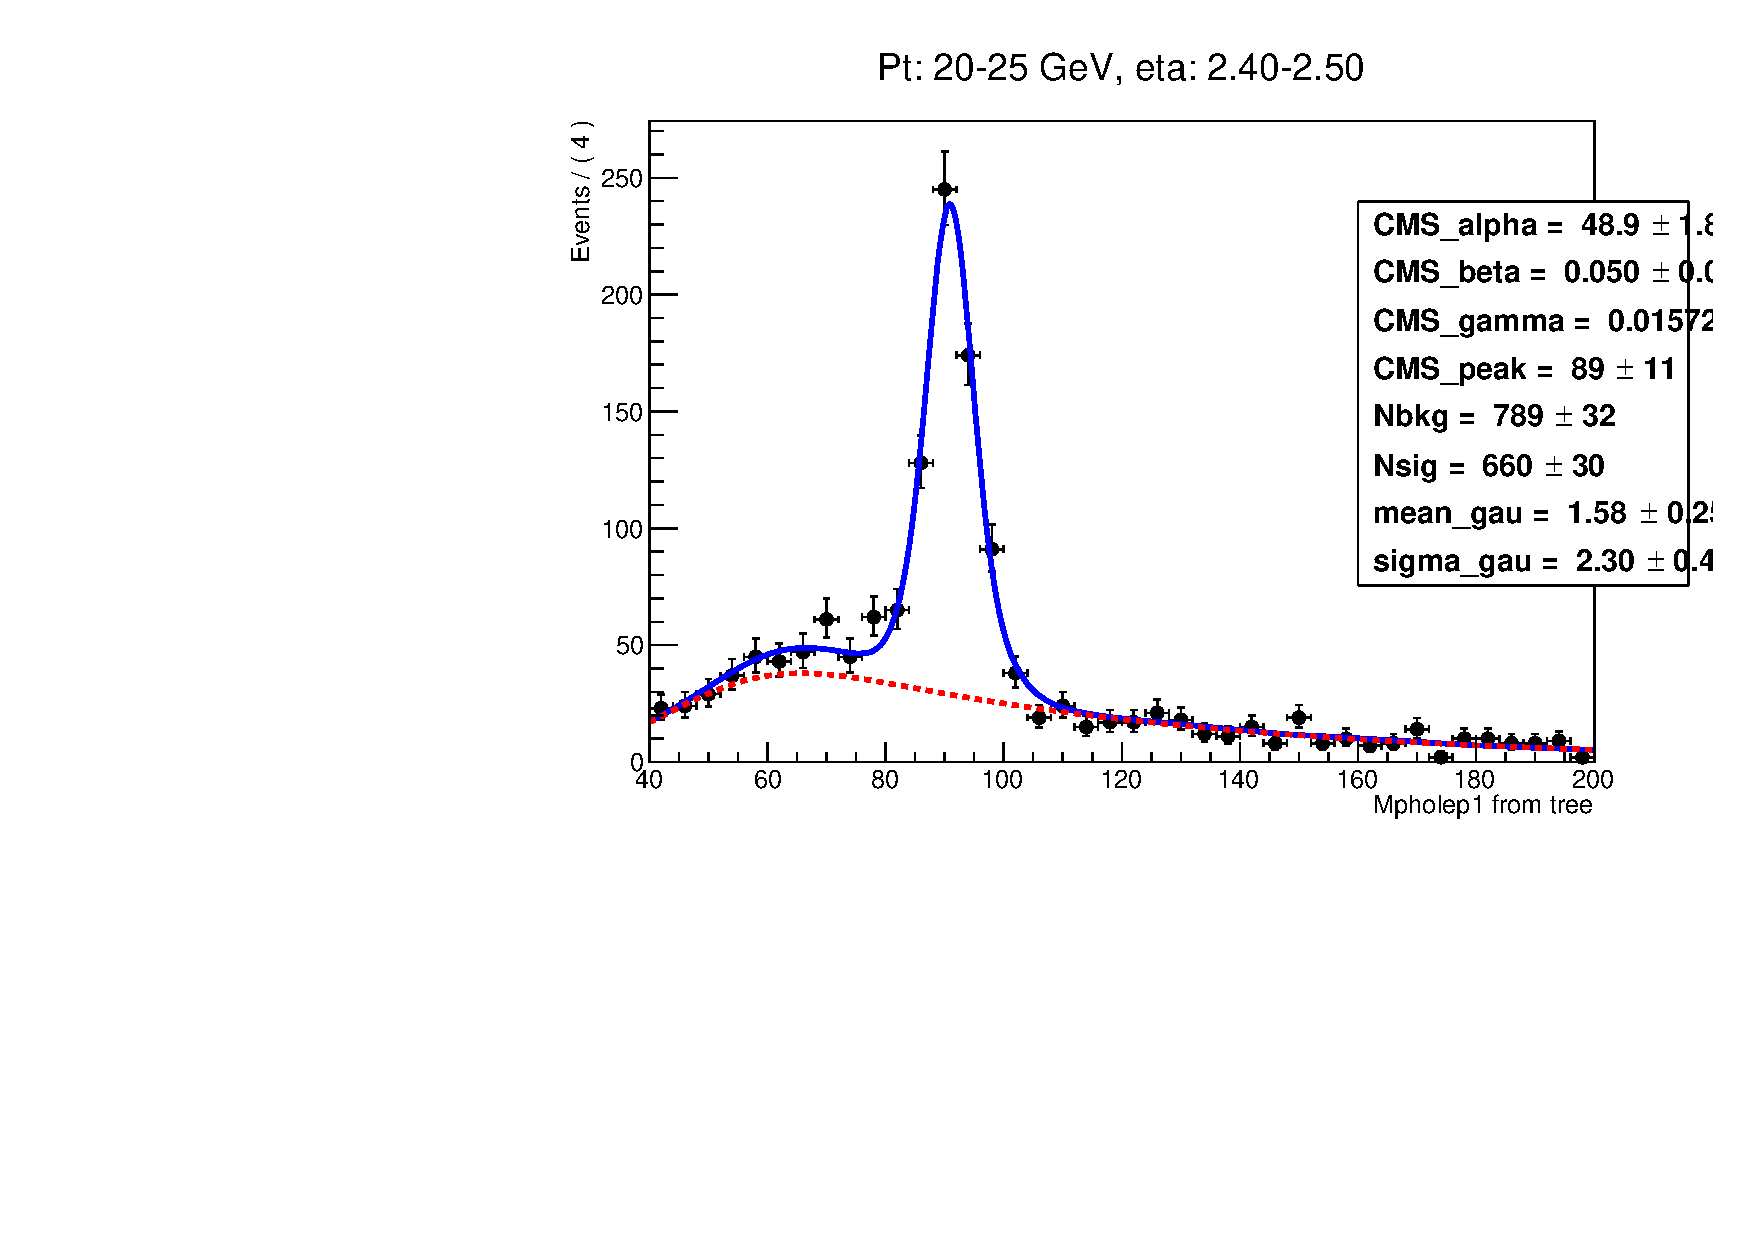
\includegraphics[width=0.45\textwidth]{../figs/figs_v11/ELECTRON_WGamma/EtoGammaFits/sa_hZmass_h_Data_EtoGamma_Enr_ENDCAP_pt20to25_ieta3.pdf}\\
  \label{fig:etogFits_20to25}
  \caption{$M_{e\gamma}$ fits, $W\gamma$, electron channel, 20-25 GeV, 8 $\eta^{\gamma}$ bins.}
  \end{center}
\end{figure}

\begin{figure}[htb]
  \begin{center}
   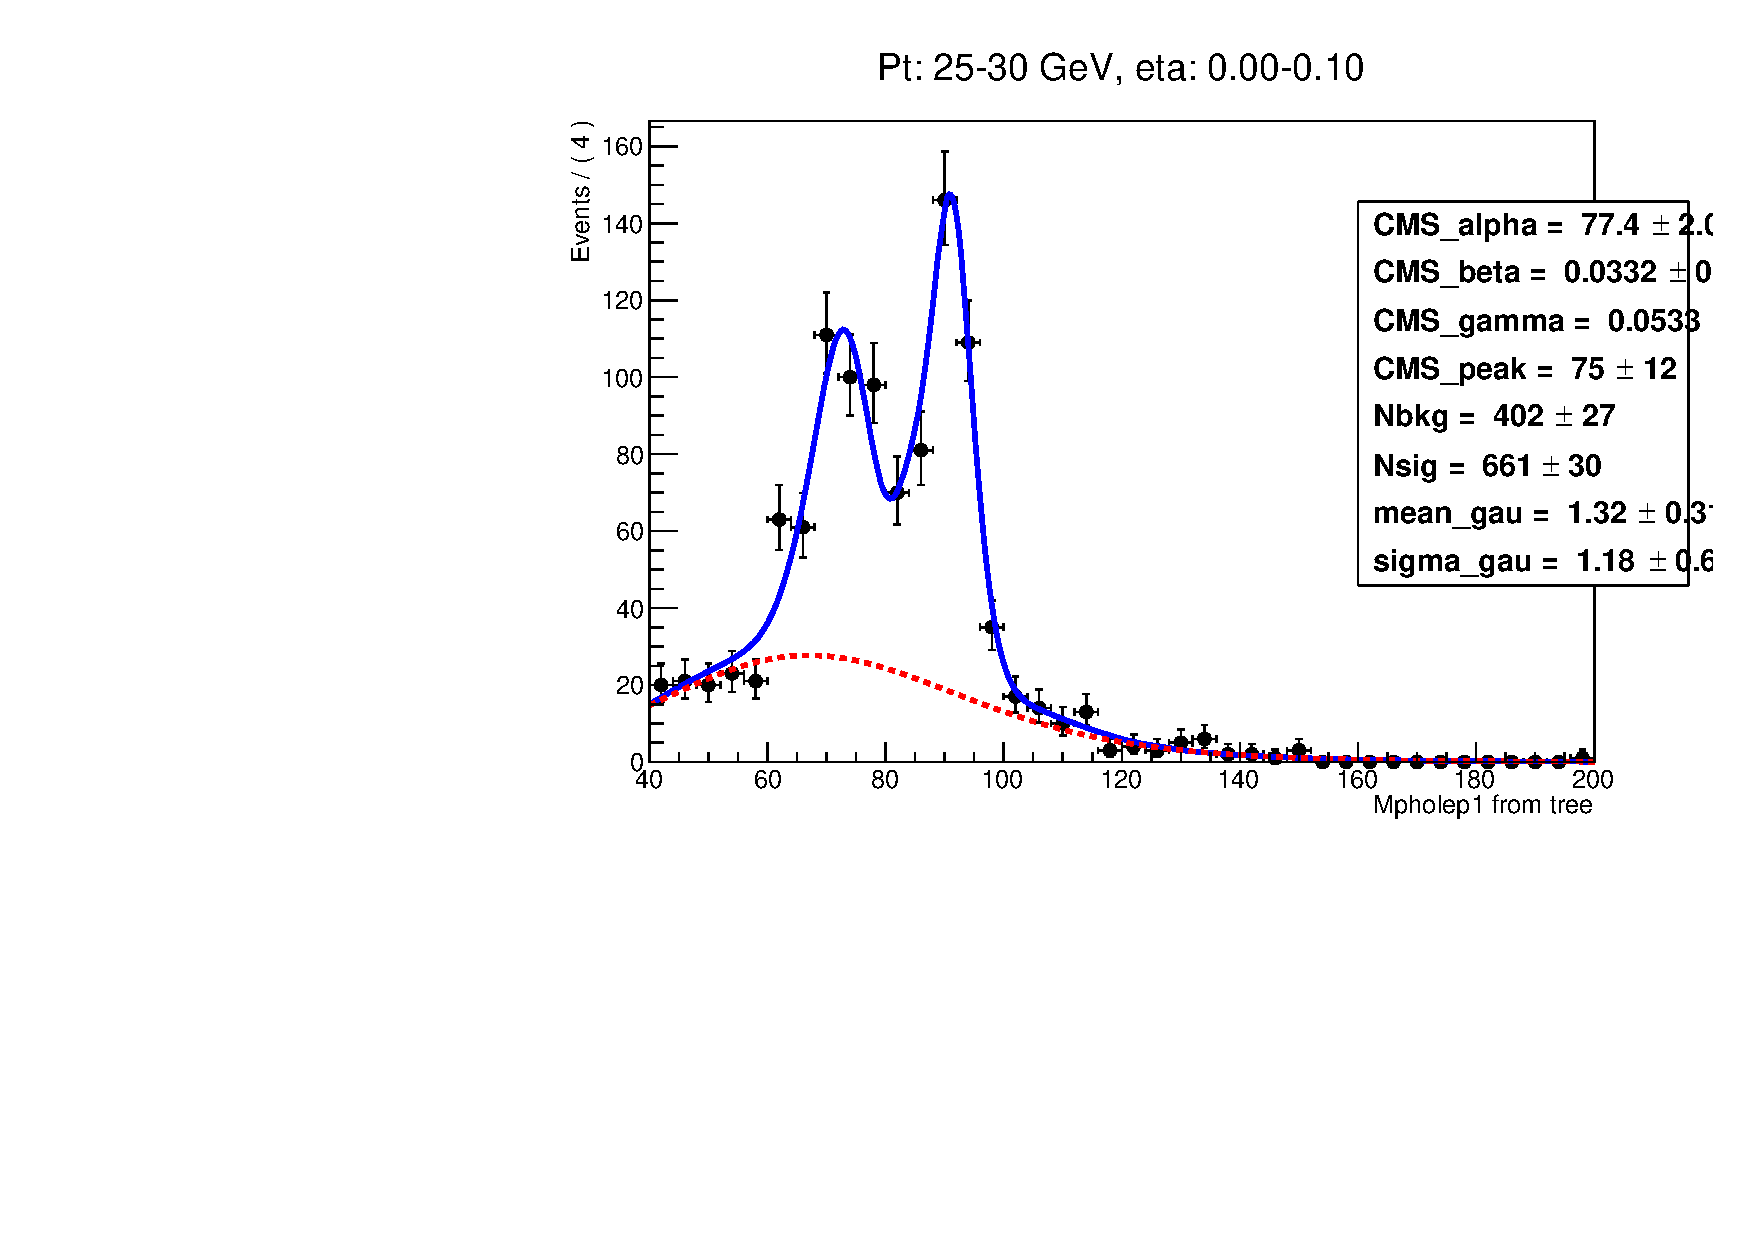
\includegraphics[width=0.45\textwidth]{../figs/figs_v11/ELECTRON_WGamma/EtoGammaFits/sa_hZmass_h_Data_EtoGamma_Enr_BARREL_pt25to30_ieta0.pdf}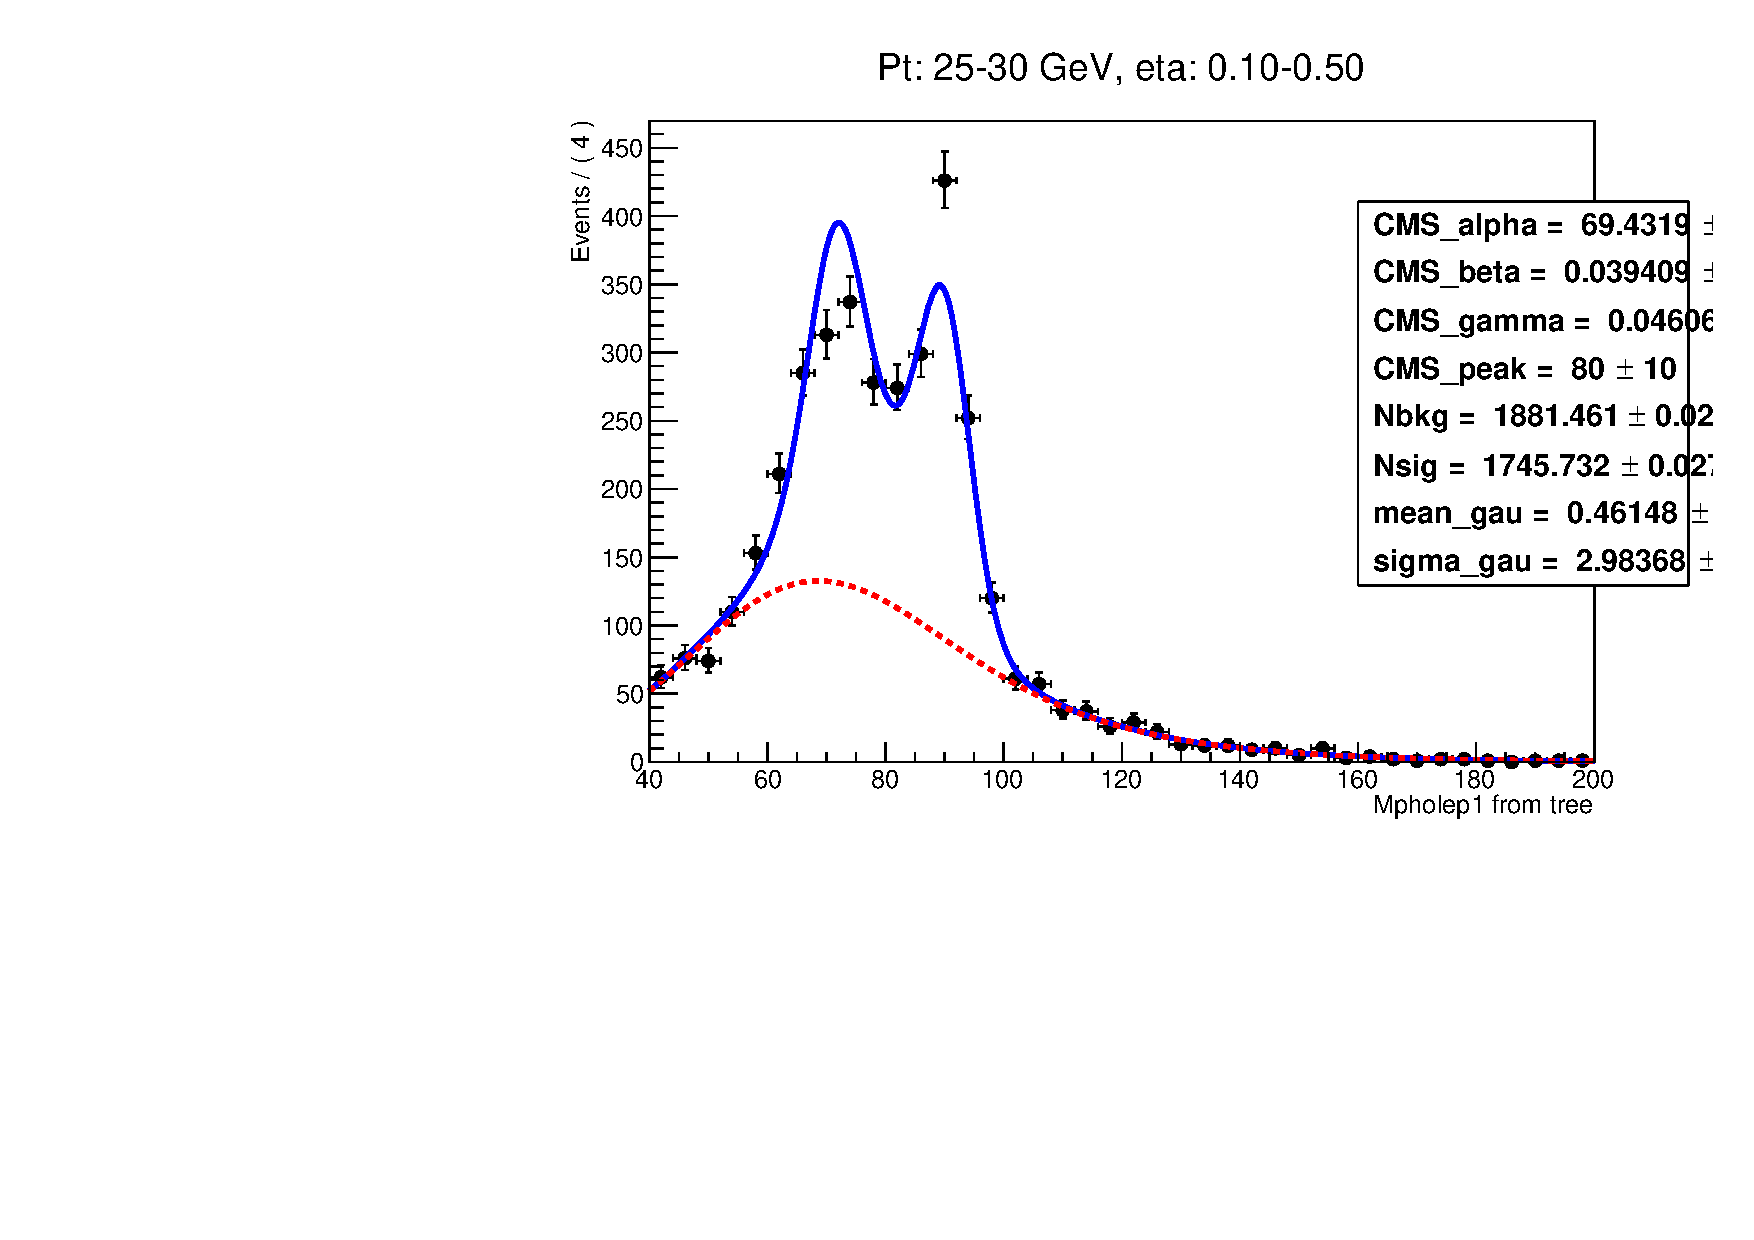
\includegraphics[width=0.45\textwidth]{../figs/figs_v11/ELECTRON_WGamma/EtoGammaFits/sa_hZmass_h_Data_EtoGamma_Enr_BARREL_pt25to30_ieta1.pdf}\\
   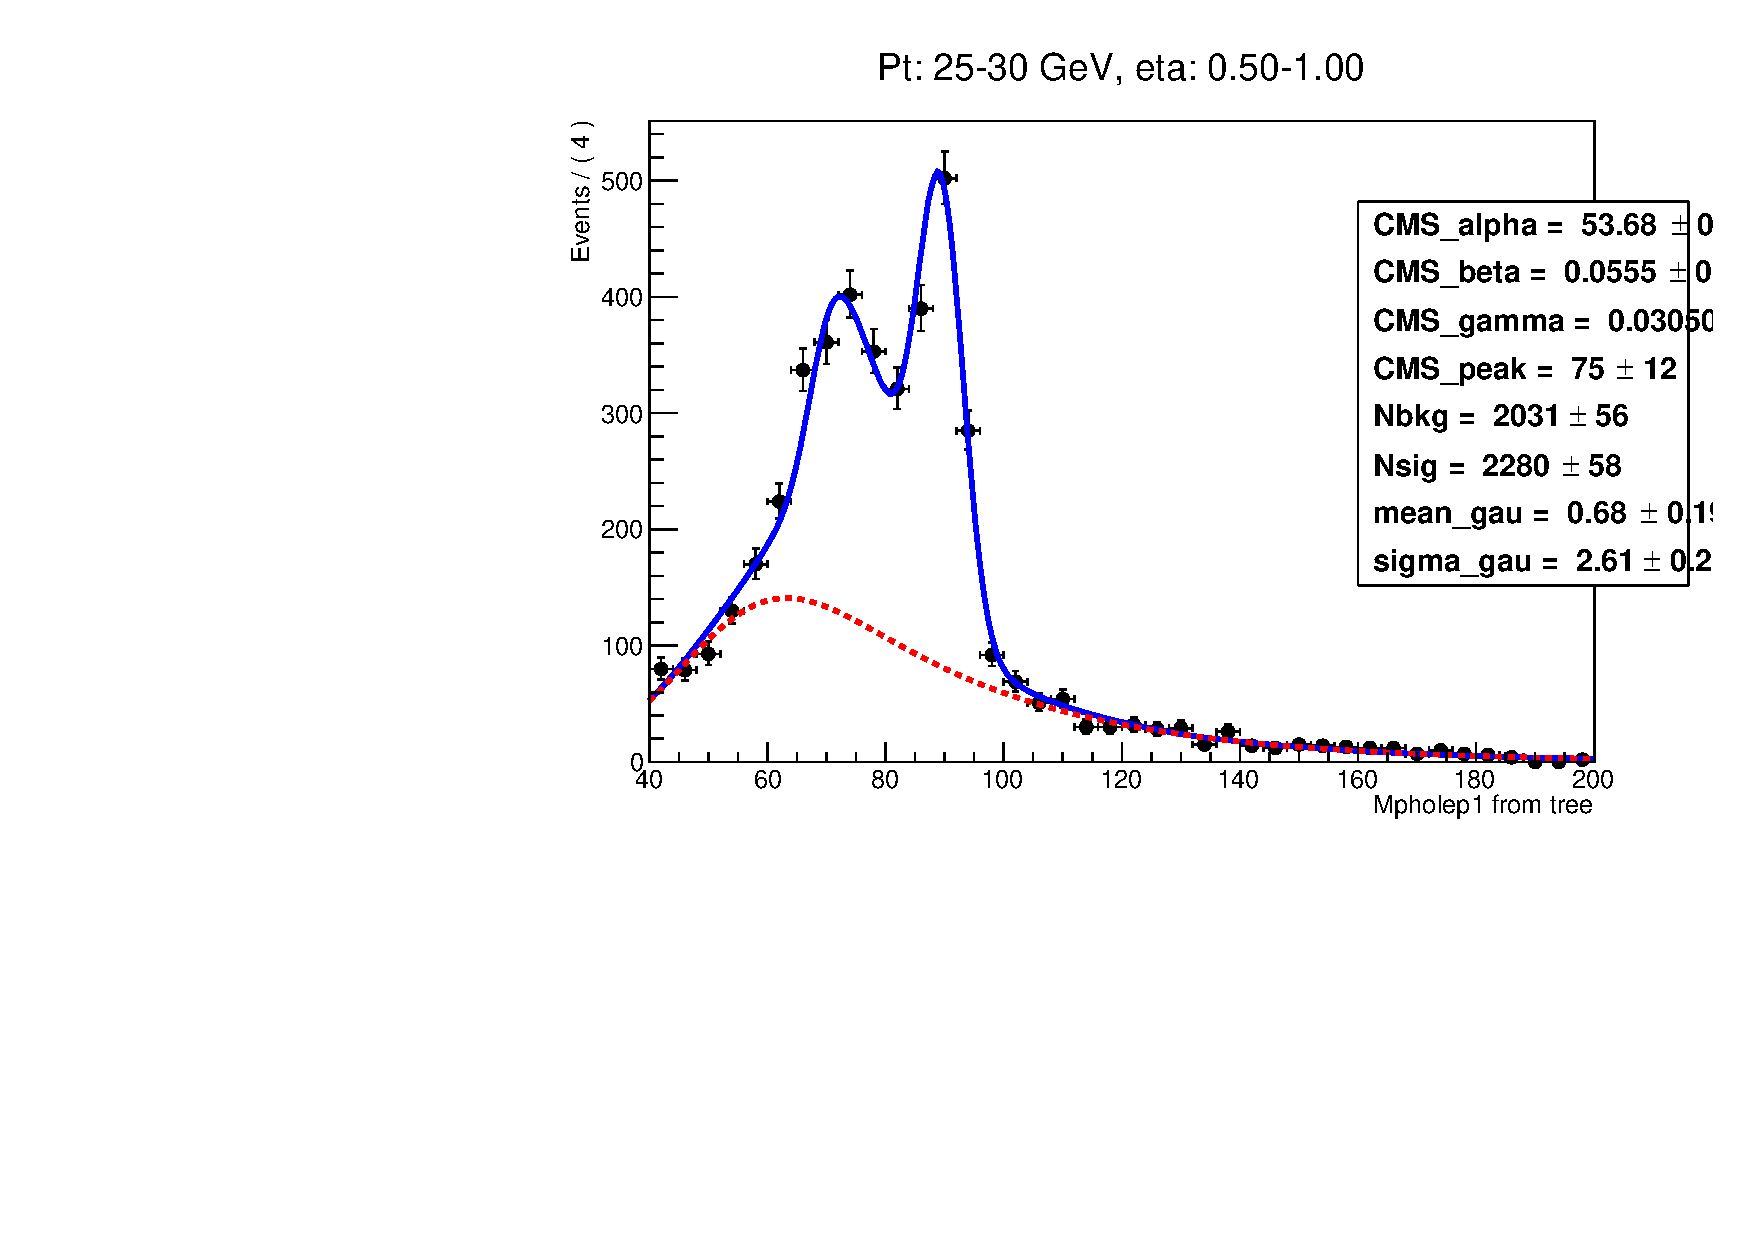
\includegraphics[width=0.45\textwidth]{../figs/figs_v11/ELECTRON_WGamma/EtoGammaFits/sa_hZmass_h_Data_EtoGamma_Enr_BARREL_pt25to30_ieta2.pdf}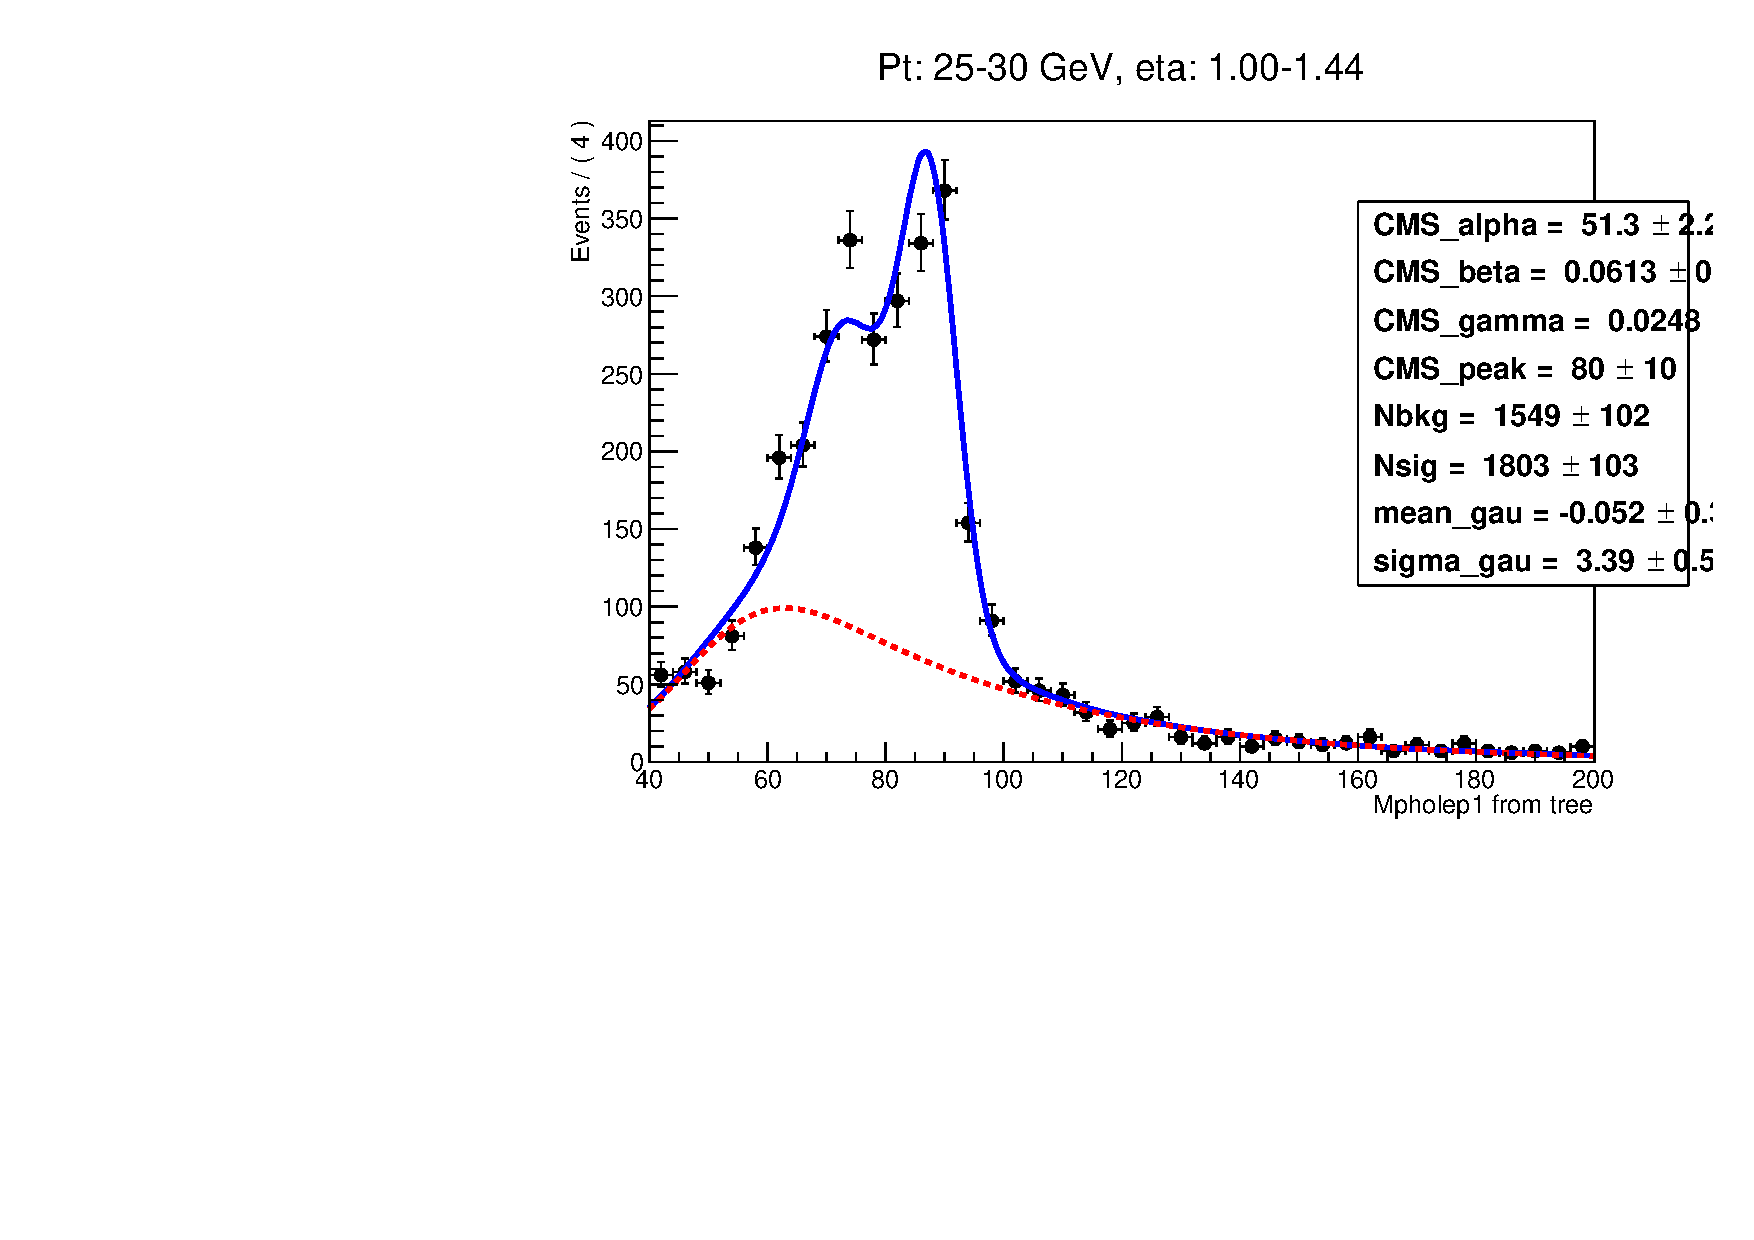
\includegraphics[width=0.45\textwidth]{../figs/figs_v11/ELECTRON_WGamma/EtoGammaFits/sa_hZmass_h_Data_EtoGamma_Enr_BARREL_pt25to30_ieta3.pdf}\\
   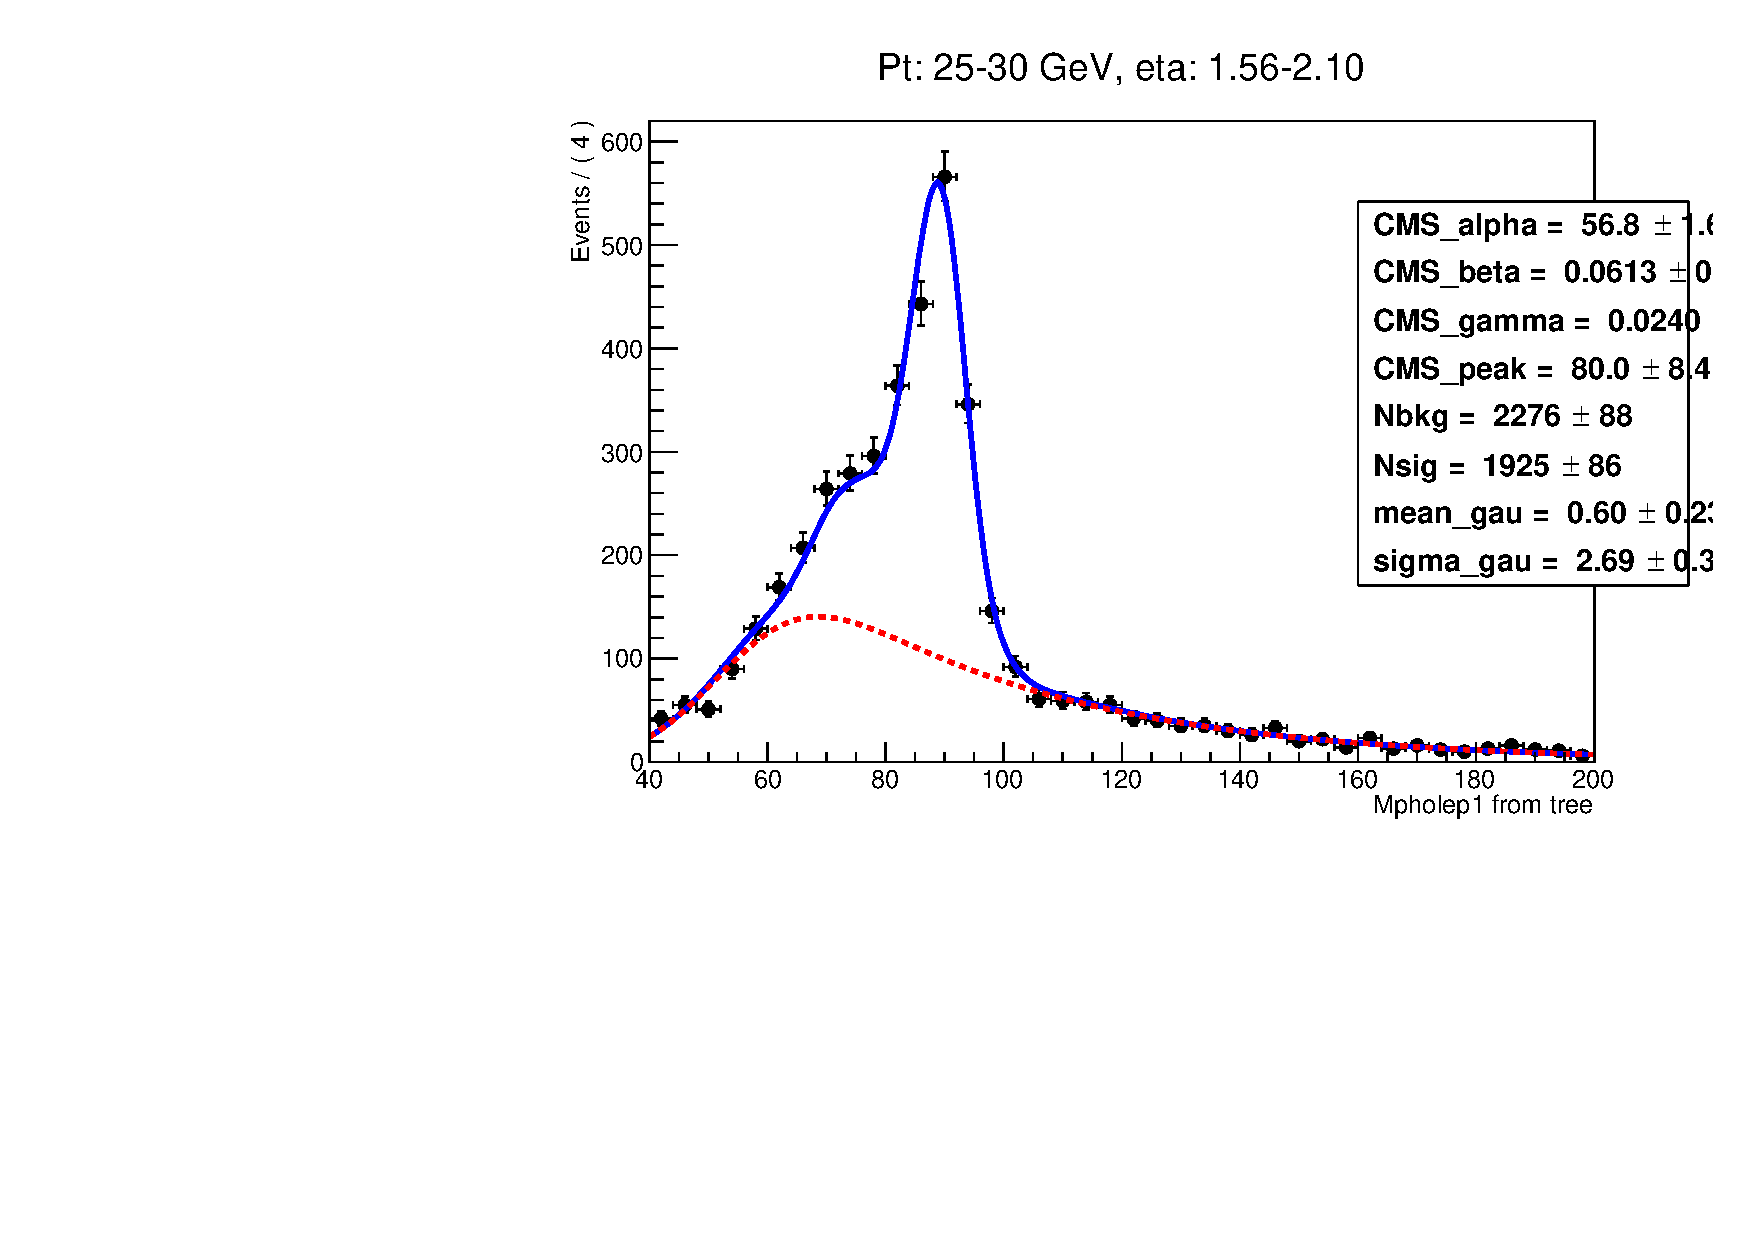
\includegraphics[width=0.45\textwidth]{../figs/figs_v11/ELECTRON_WGamma/EtoGammaFits/sa_hZmass_h_Data_EtoGamma_Enr_ENDCAP_pt25to30_ieta0.pdf}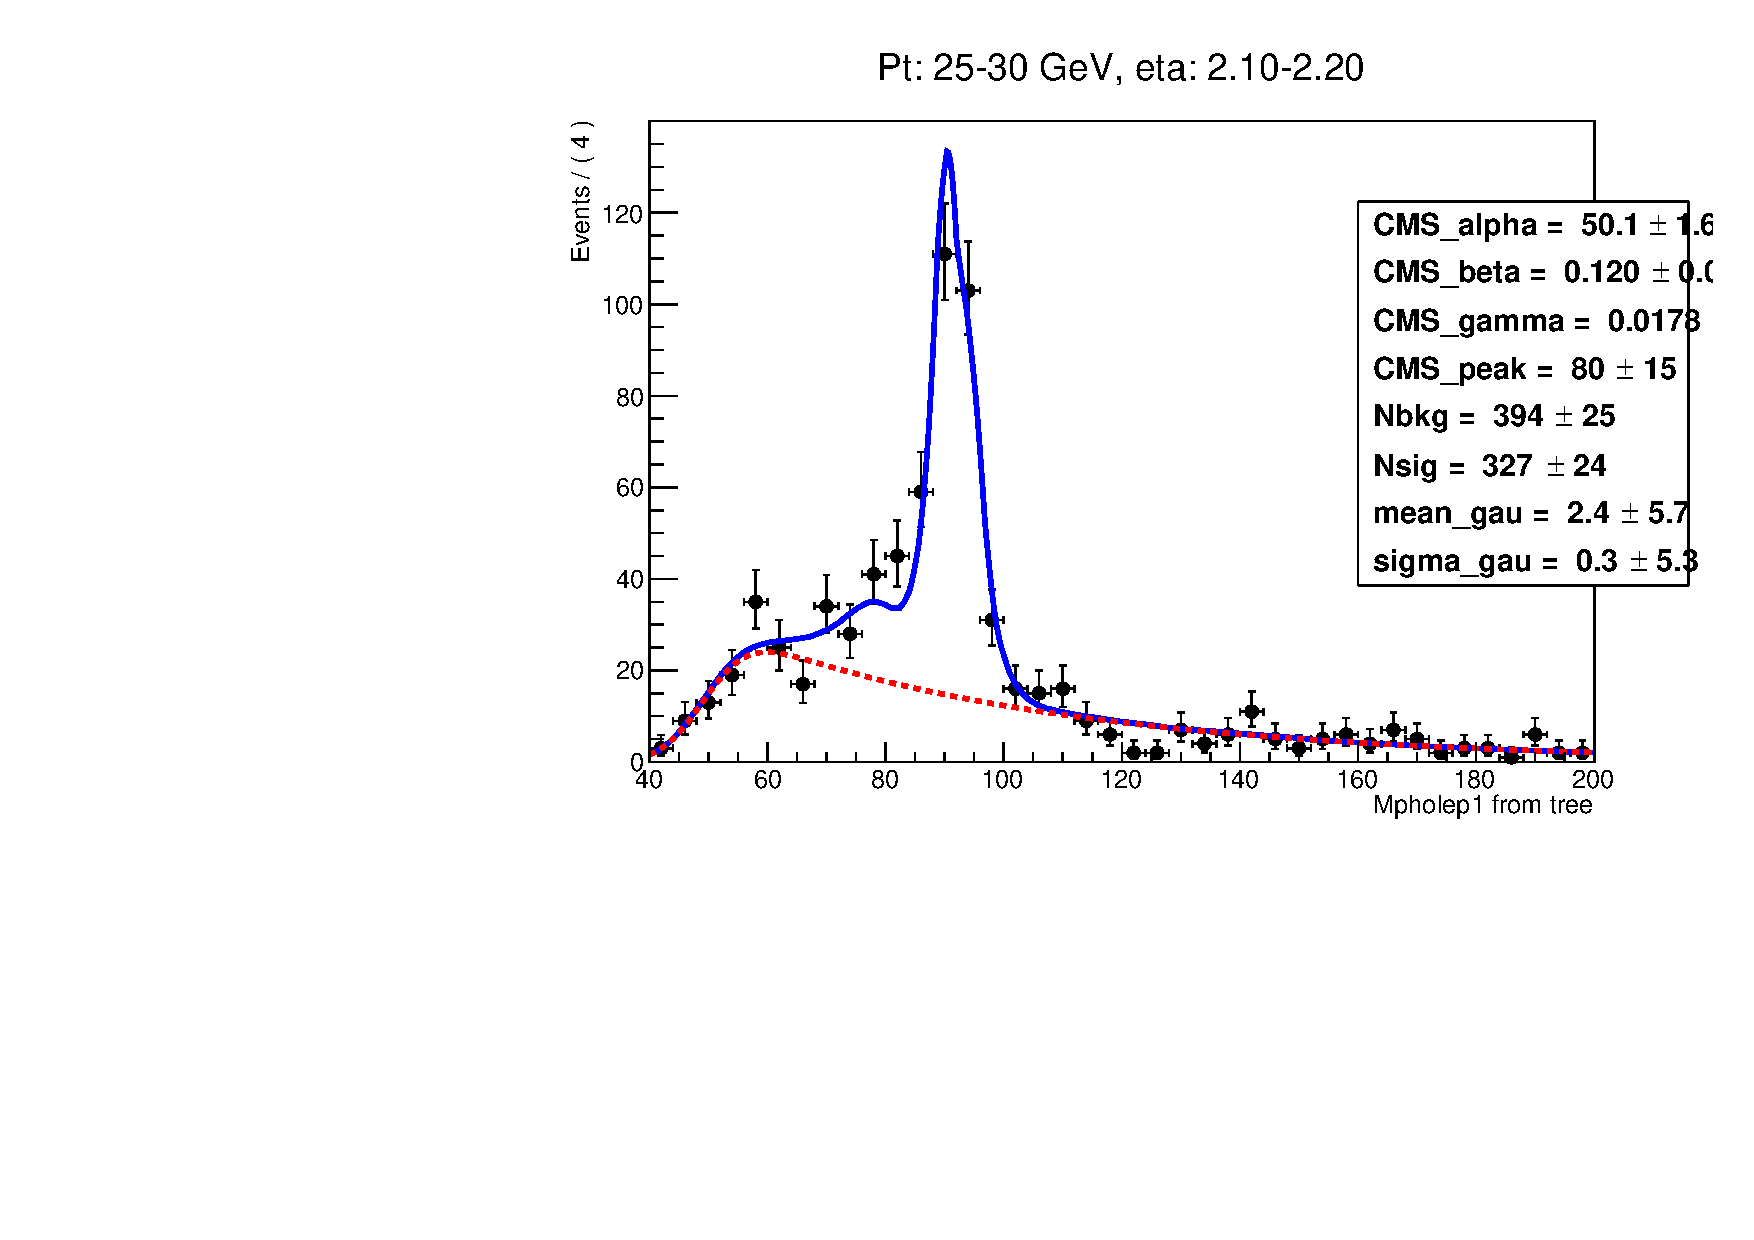
\includegraphics[width=0.45\textwidth]{../figs/figs_v11/ELECTRON_WGamma/EtoGammaFits/sa_hZmass_h_Data_EtoGamma_Enr_ENDCAP_pt25to30_ieta1.pdf}\\
   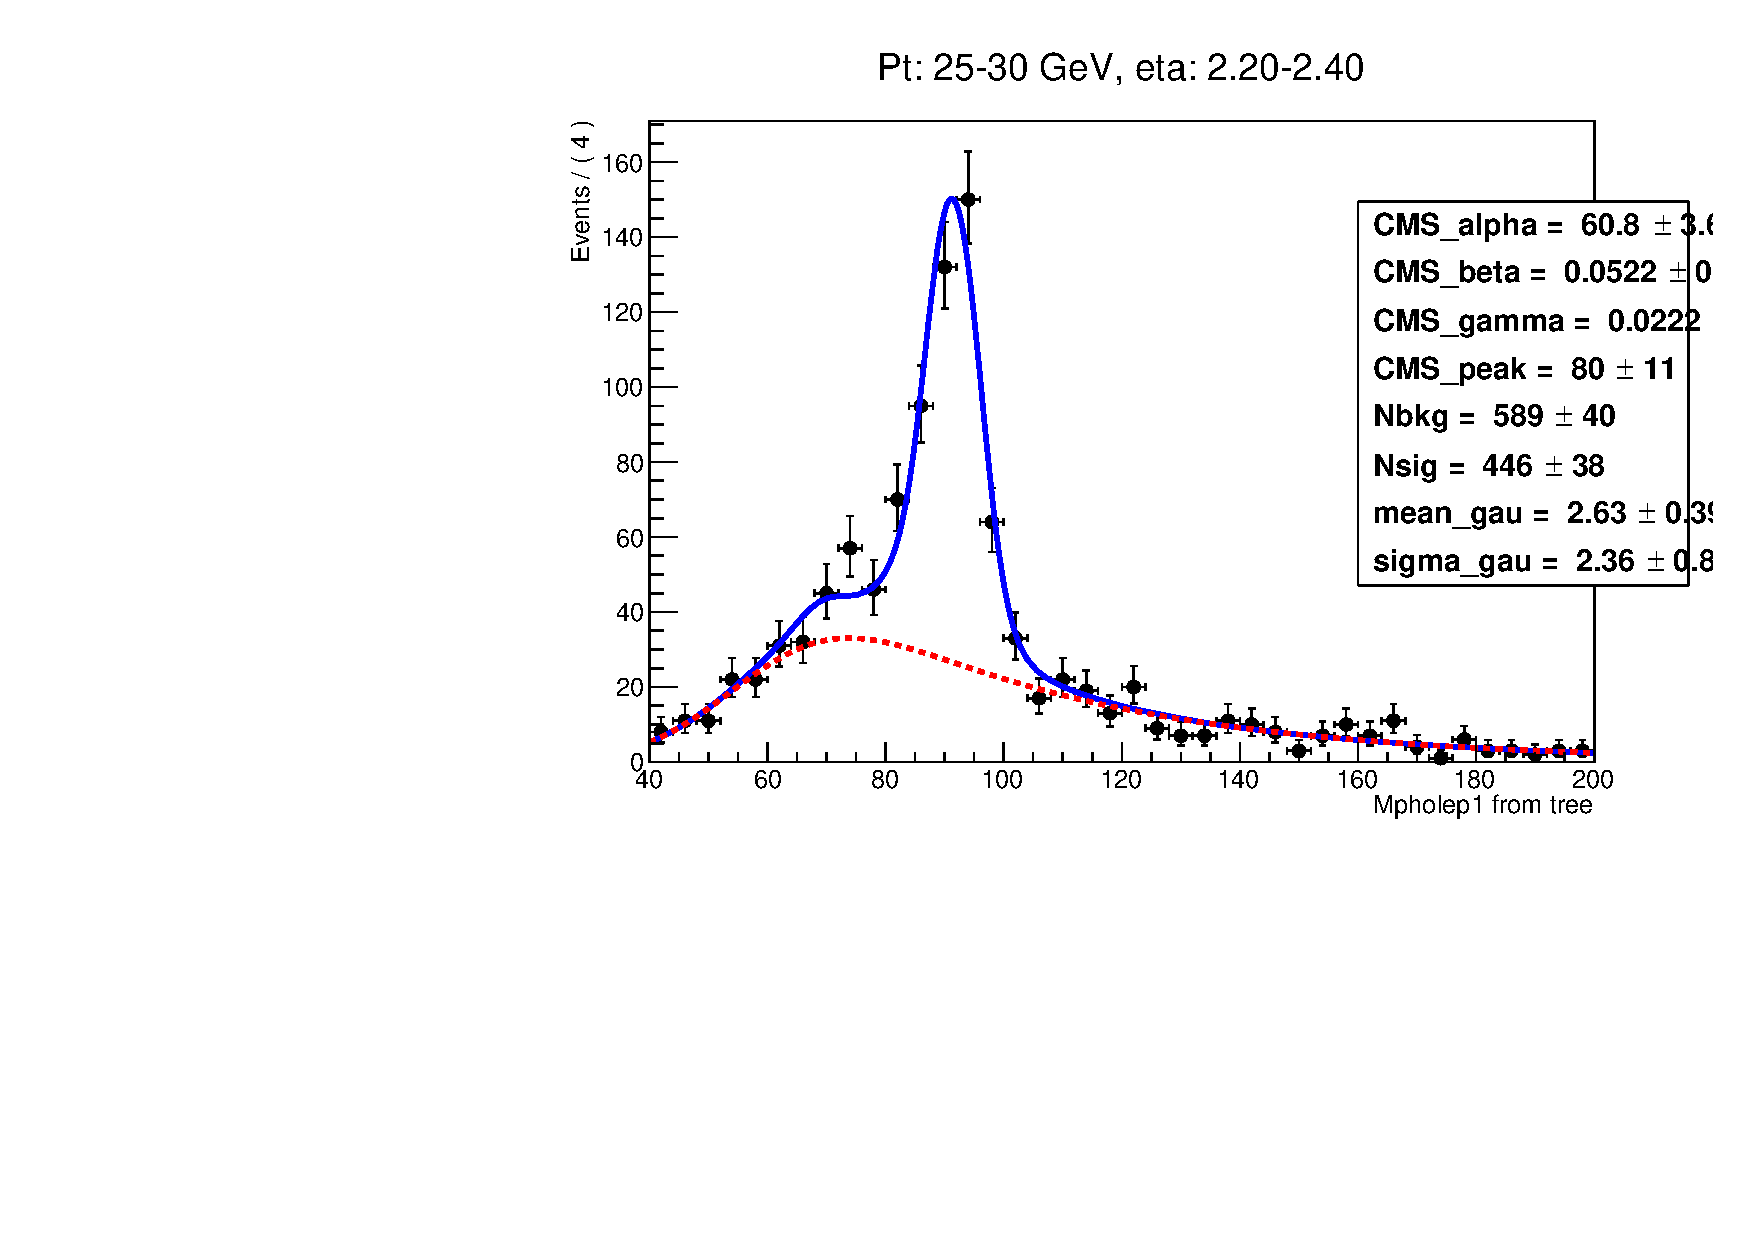
\includegraphics[width=0.45\textwidth]{../figs/figs_v11/ELECTRON_WGamma/EtoGammaFits/sa_hZmass_h_Data_EtoGamma_Enr_ENDCAP_pt25to30_ieta2.pdf}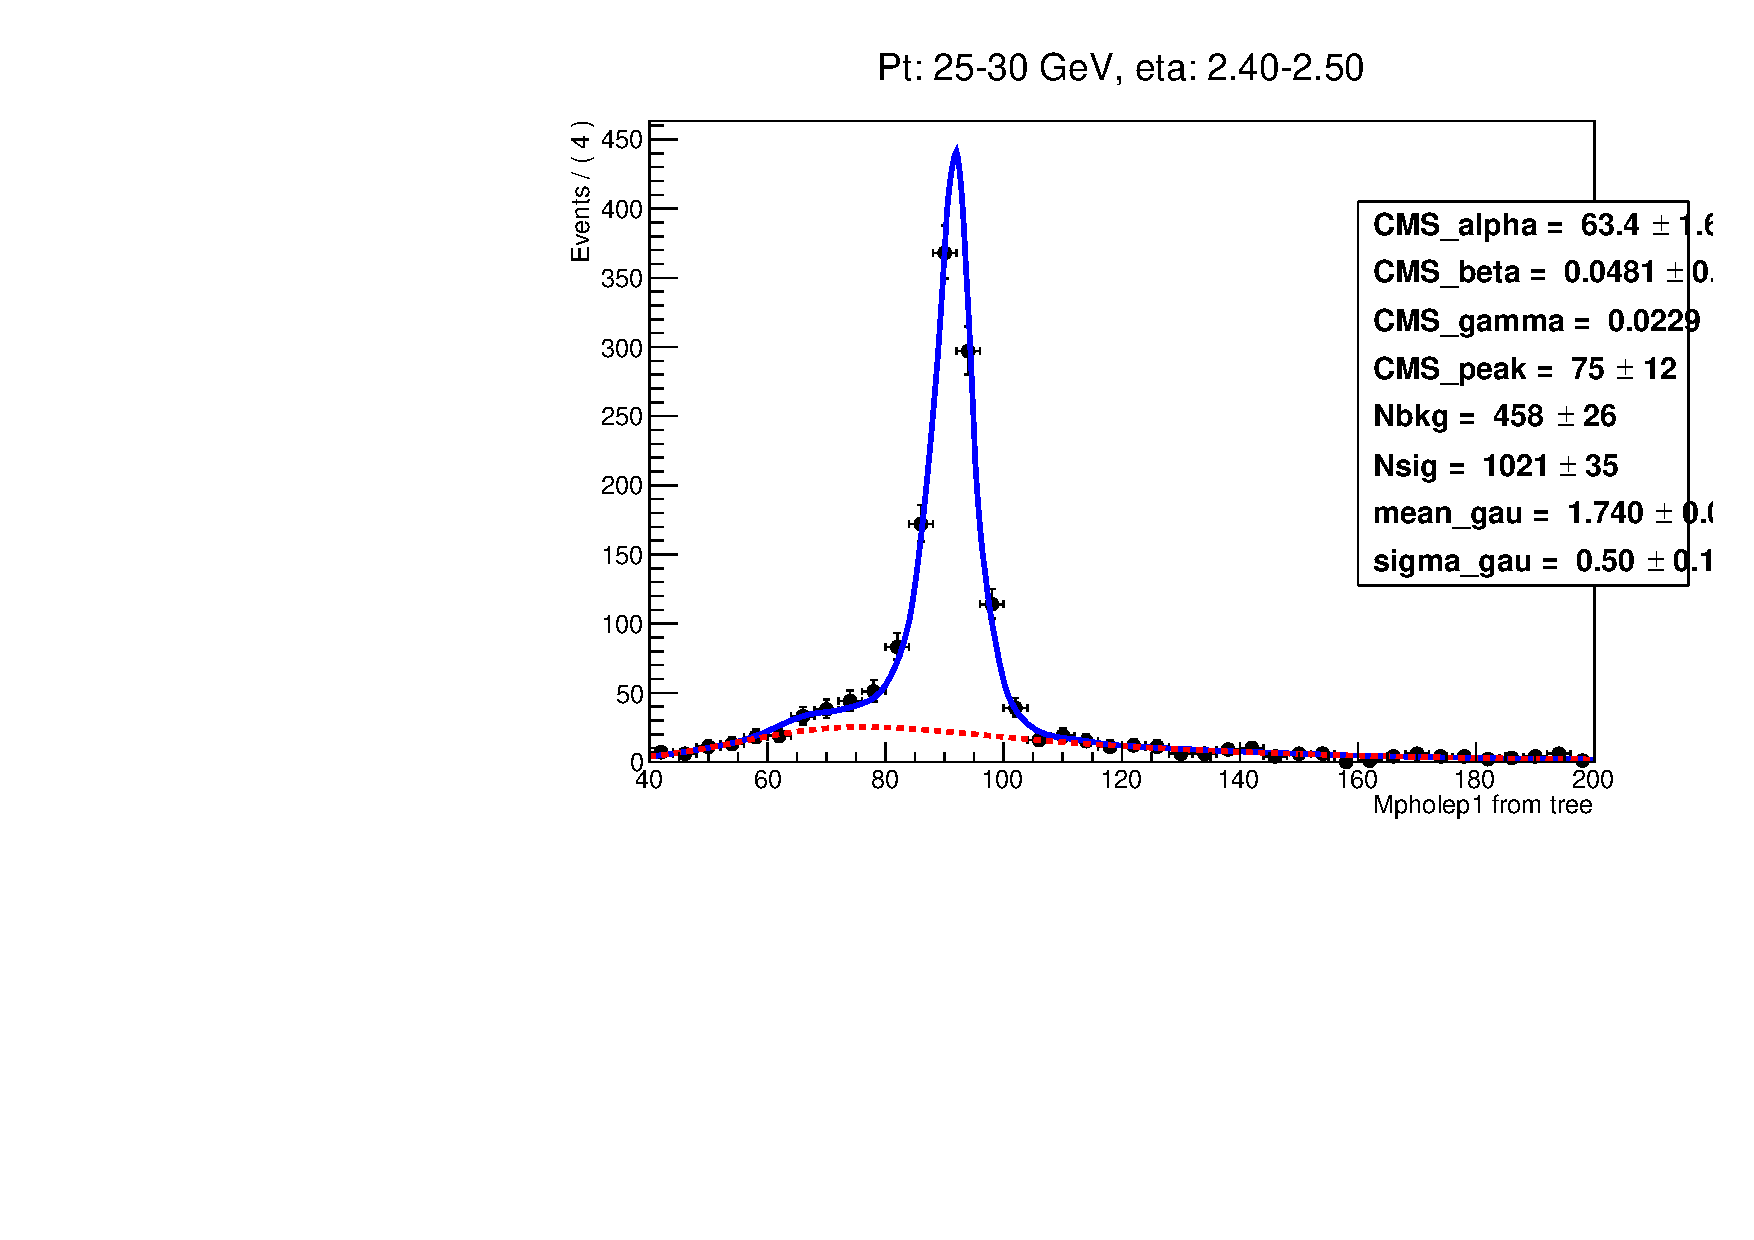
\includegraphics[width=0.45\textwidth]{../figs/figs_v11/ELECTRON_WGamma/EtoGammaFits/sa_hZmass_h_Data_EtoGamma_Enr_ENDCAP_pt25to30_ieta3.pdf}\\
  \label{fig:etogFits_25to30}
  \caption{$M_{e\gamma}$ fits, $W\gamma$, electron channel, 25-30 GeV, 8 $\eta^{\gamma}$ bins.}
  \end{center}
\end{figure}

\begin{figure}[htb]
  \begin{center}
   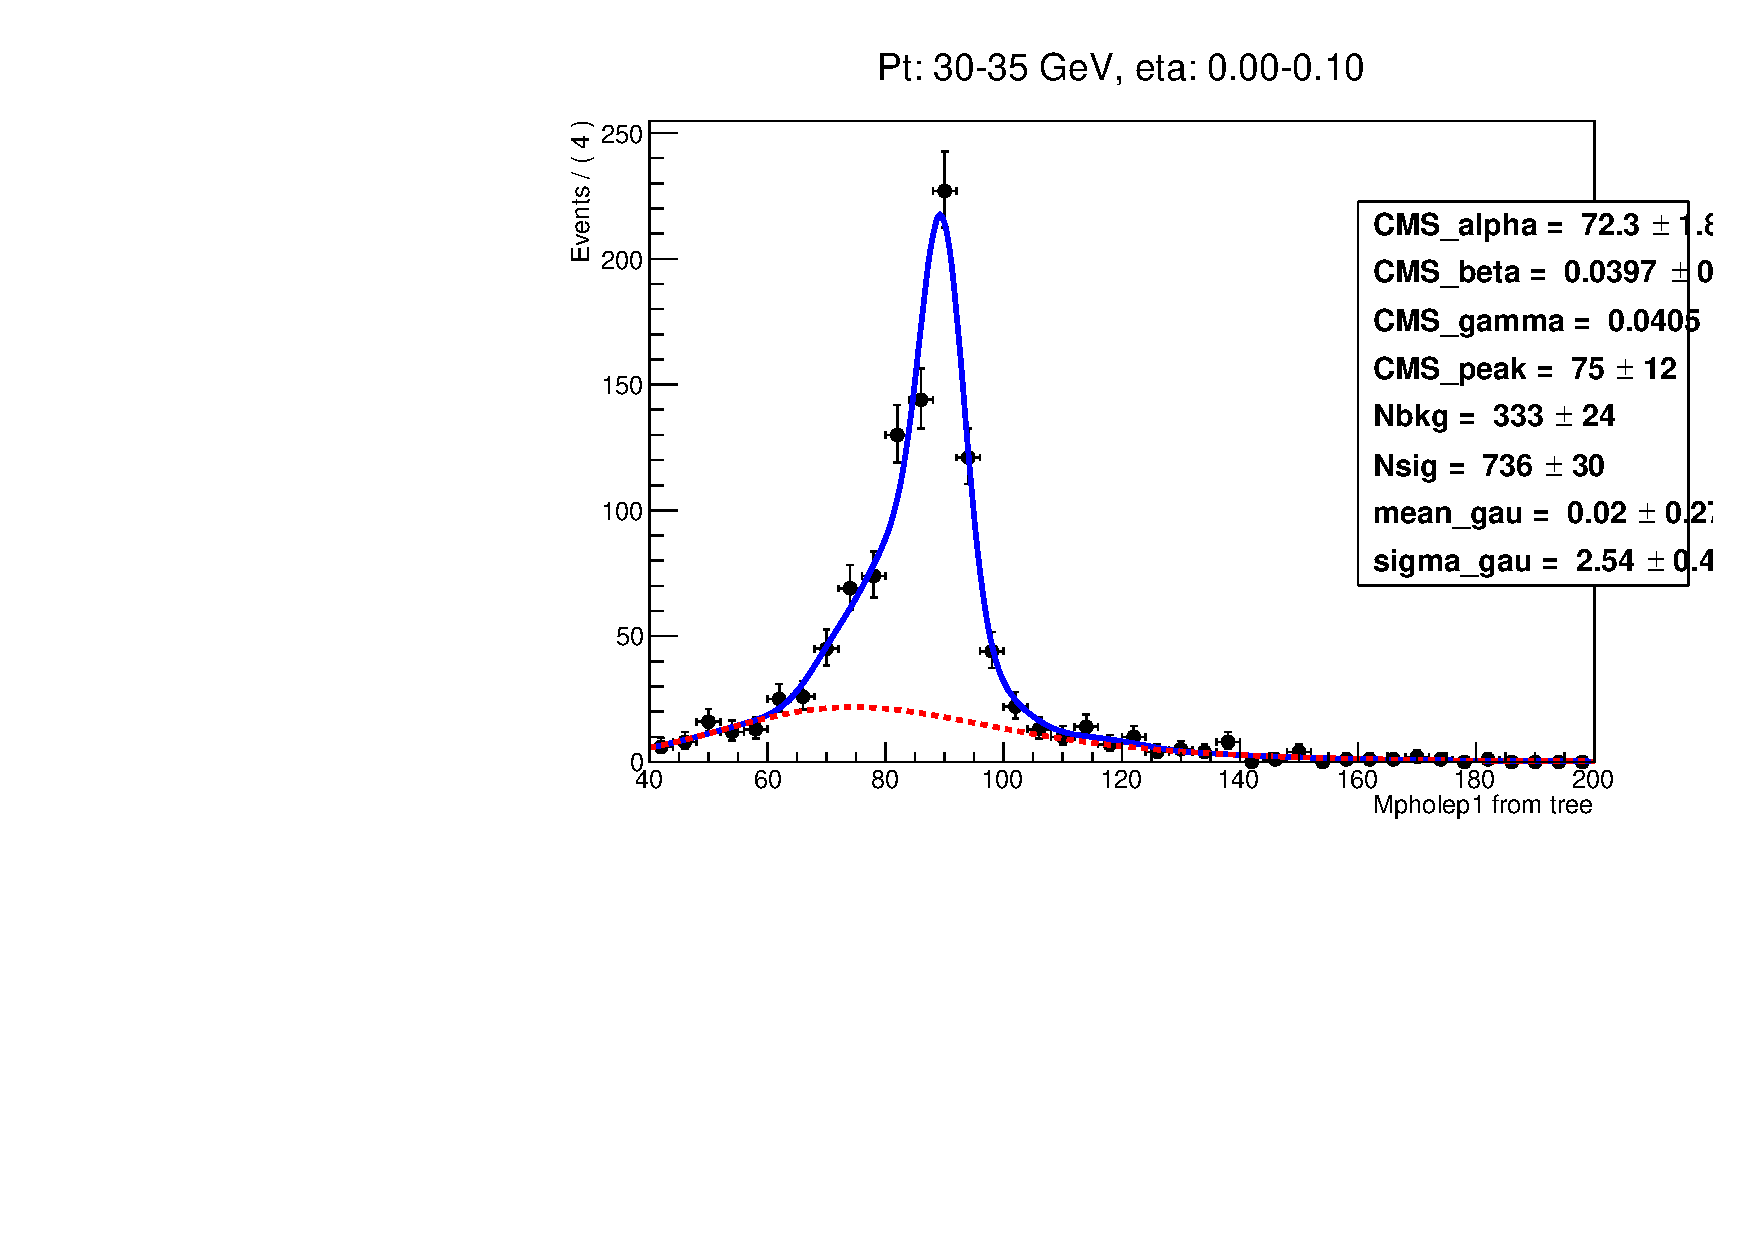
\includegraphics[width=0.45\textwidth]{../figs/figs_v11/ELECTRON_WGamma/EtoGammaFits/sa_hZmass_h_Data_EtoGamma_Enr_BARREL_pt30to35_ieta0.pdf}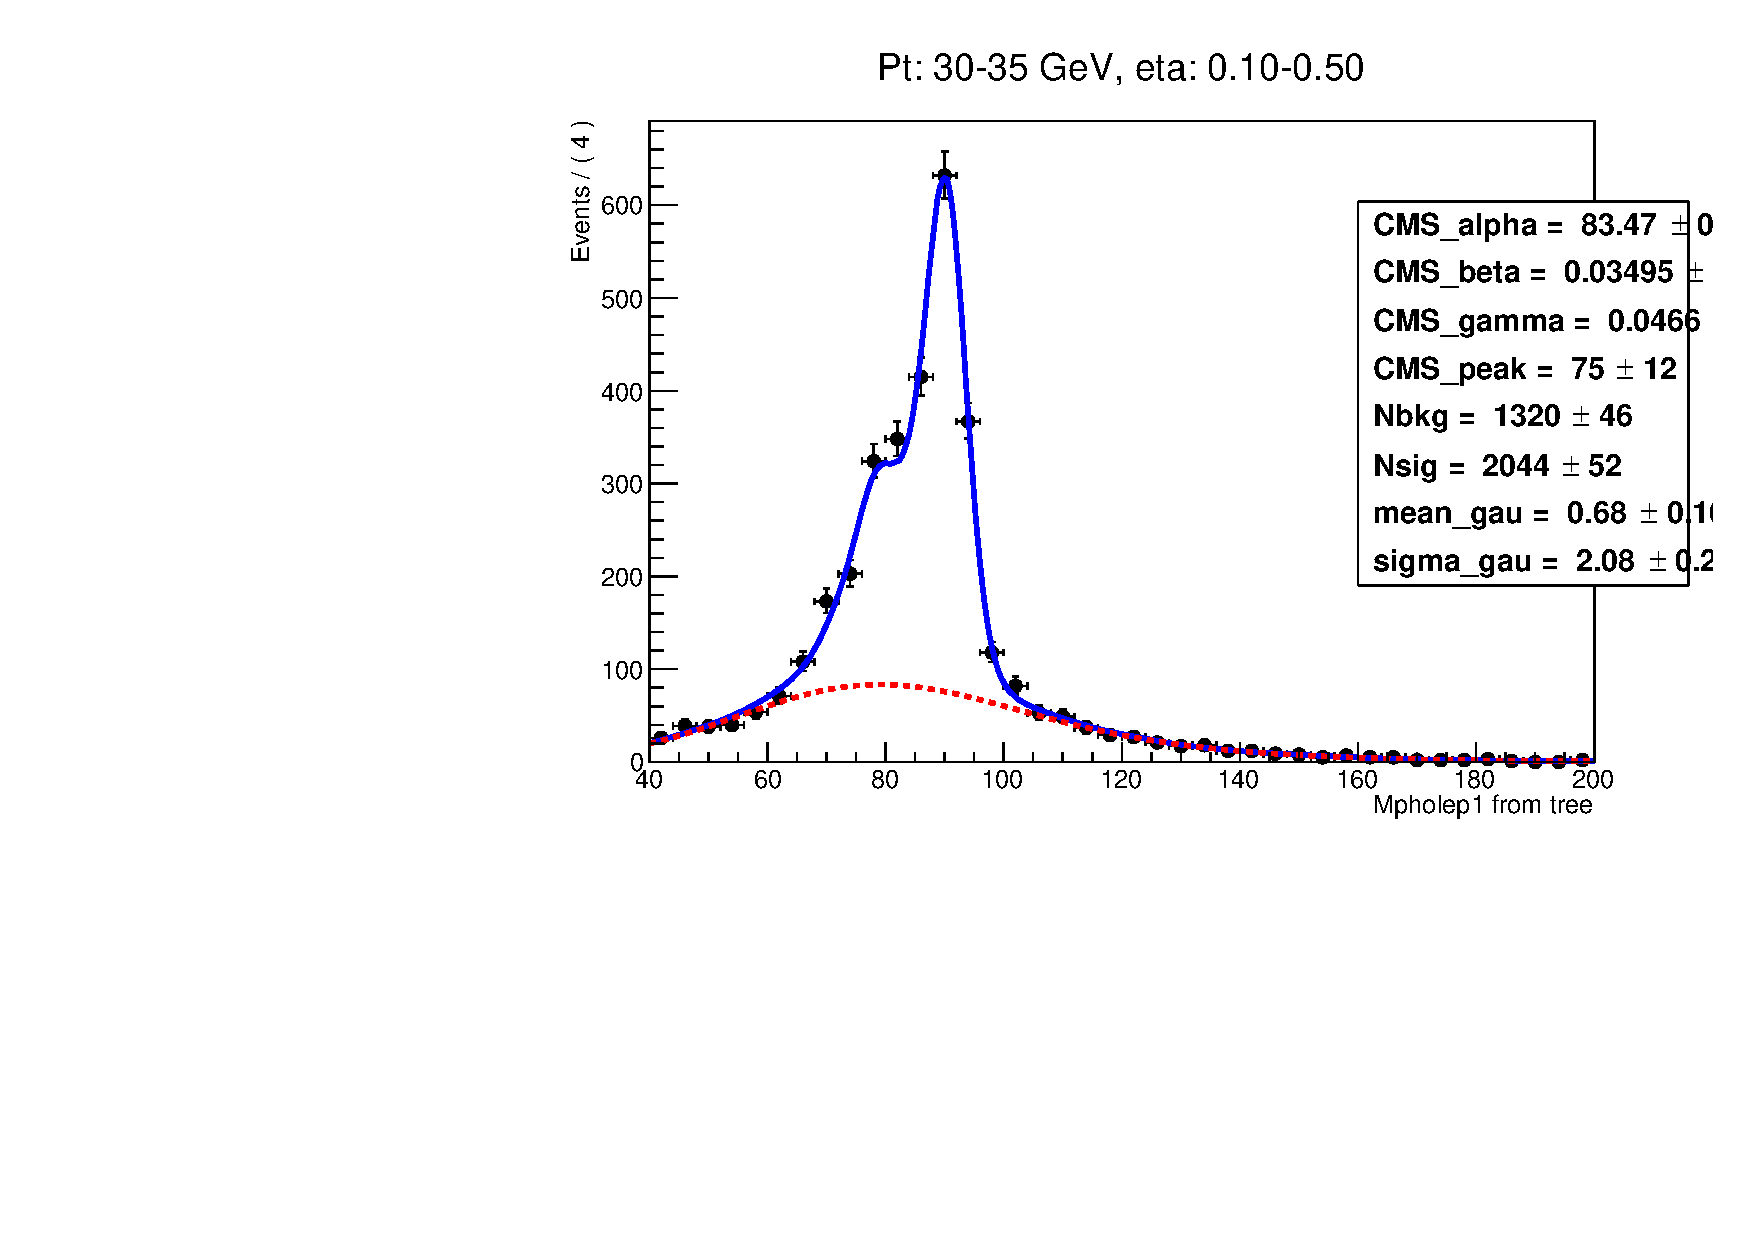
\includegraphics[width=0.45\textwidth]{../figs/figs_v11/ELECTRON_WGamma/EtoGammaFits/sa_hZmass_h_Data_EtoGamma_Enr_BARREL_pt30to35_ieta1.pdf}\\
   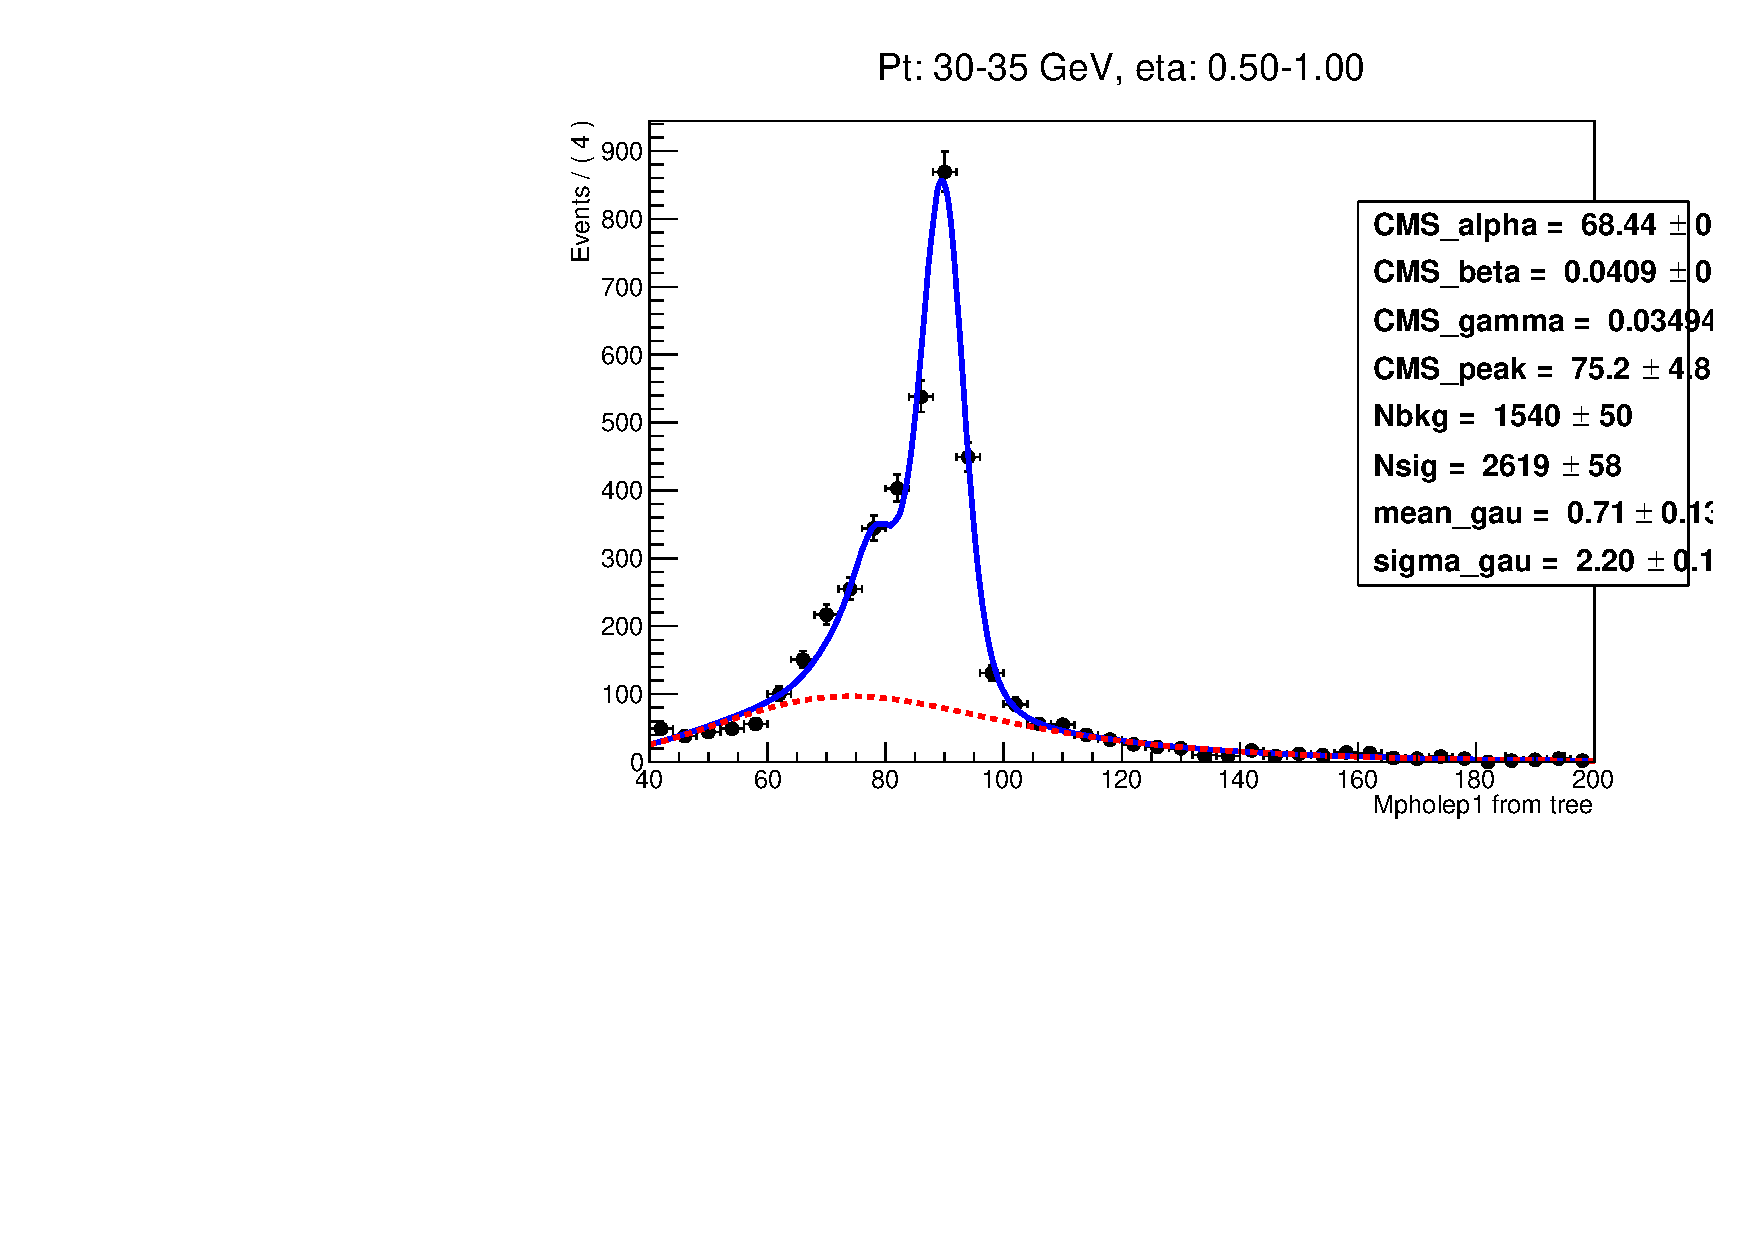
\includegraphics[width=0.45\textwidth]{../figs/figs_v11/ELECTRON_WGamma/EtoGammaFits/sa_hZmass_h_Data_EtoGamma_Enr_BARREL_pt30to35_ieta2.pdf}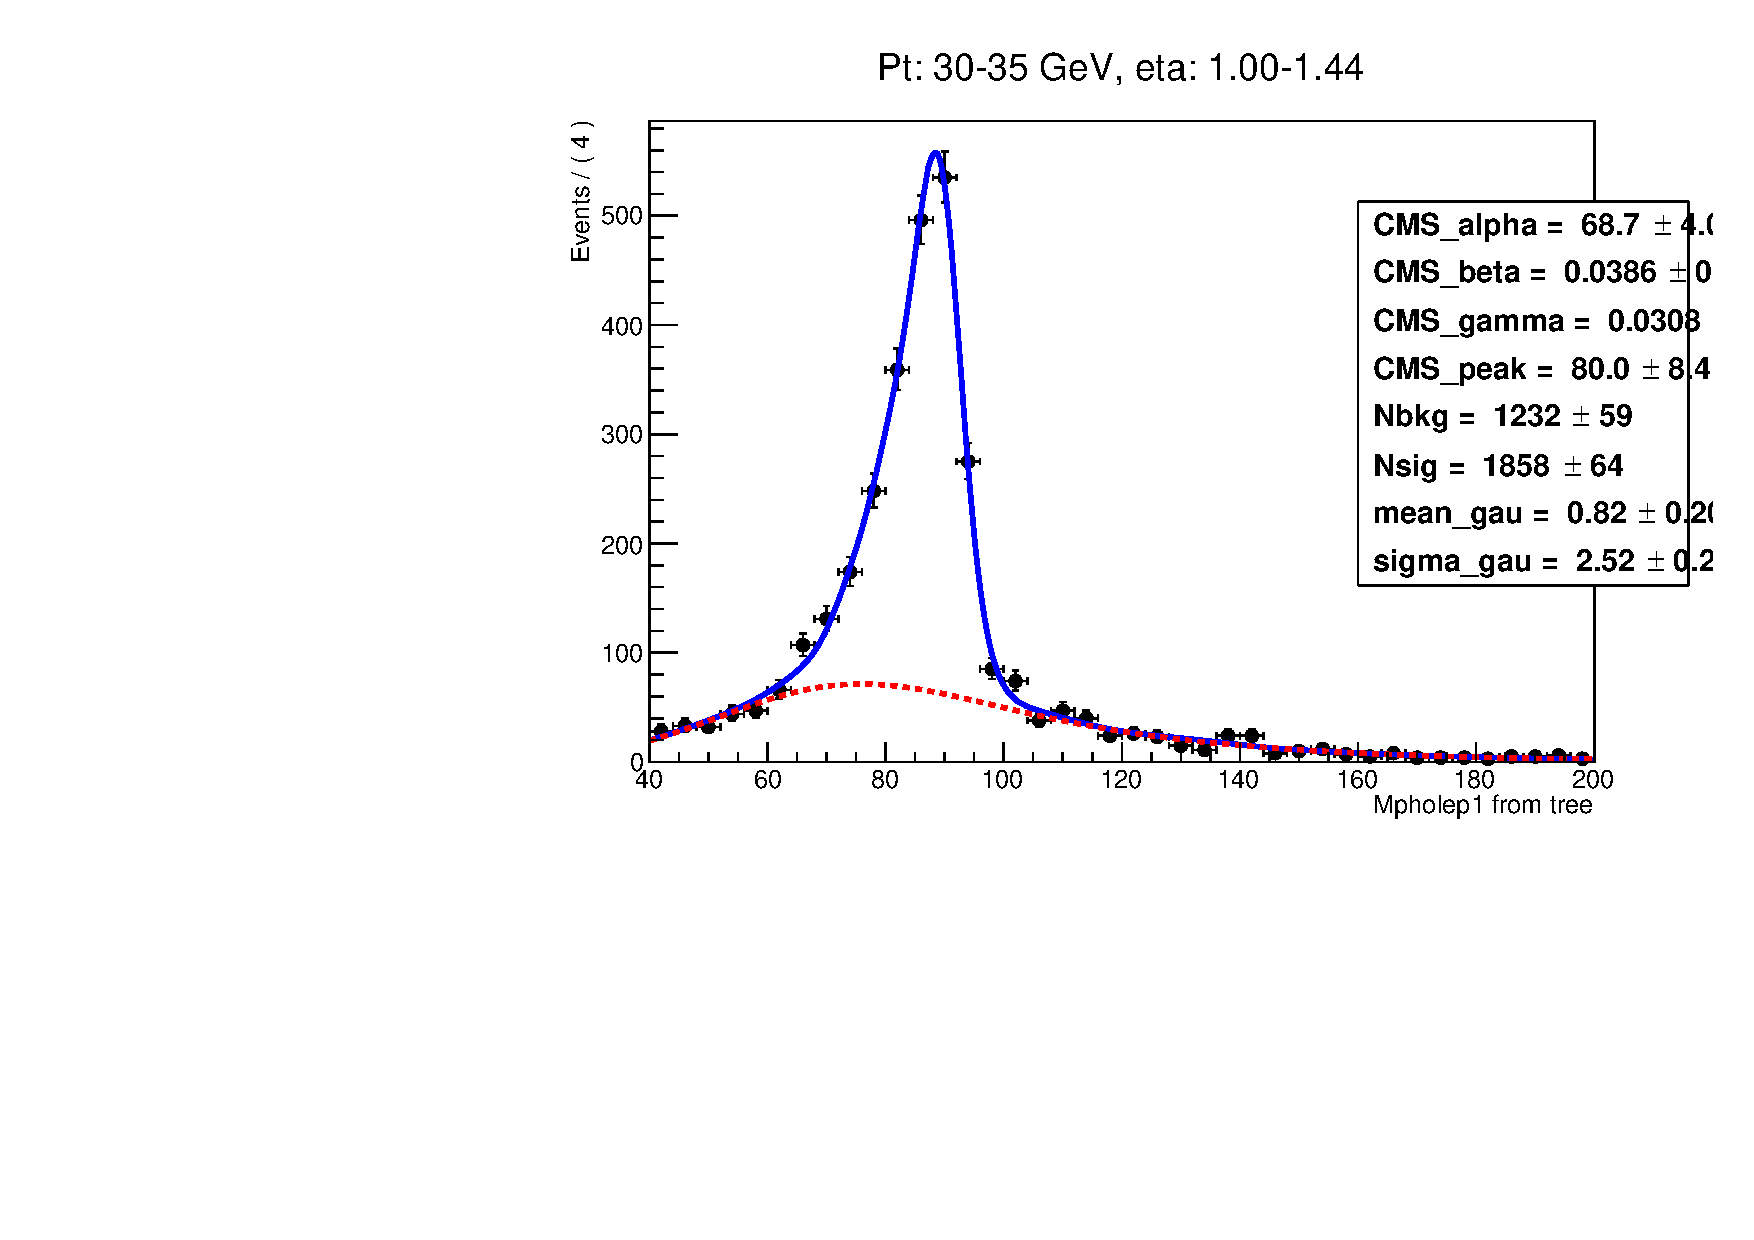
\includegraphics[width=0.45\textwidth]{../figs/figs_v11/ELECTRON_WGamma/EtoGammaFits/sa_hZmass_h_Data_EtoGamma_Enr_BARREL_pt30to35_ieta3.pdf}\\
   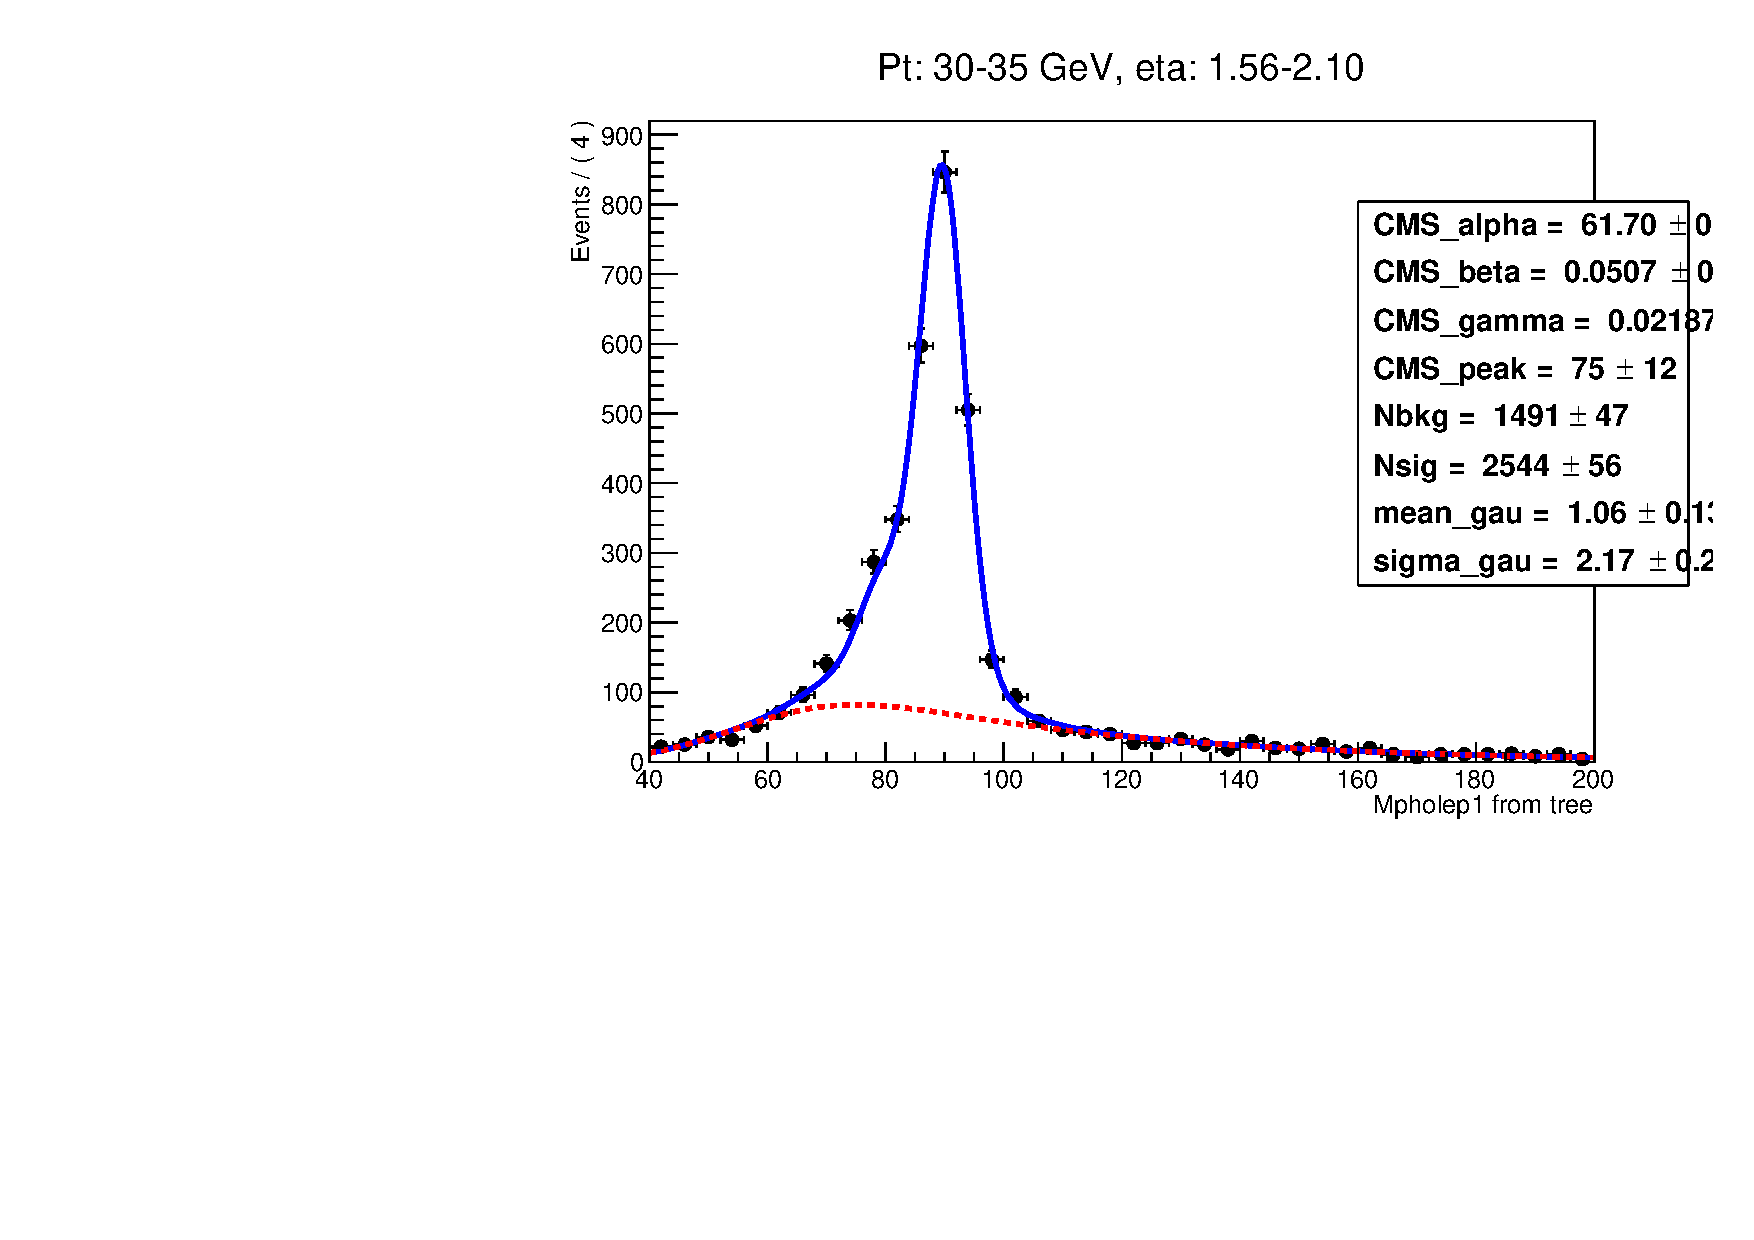
\includegraphics[width=0.45\textwidth]{../figs/figs_v11/ELECTRON_WGamma/EtoGammaFits/sa_hZmass_h_Data_EtoGamma_Enr_ENDCAP_pt30to35_ieta0.pdf}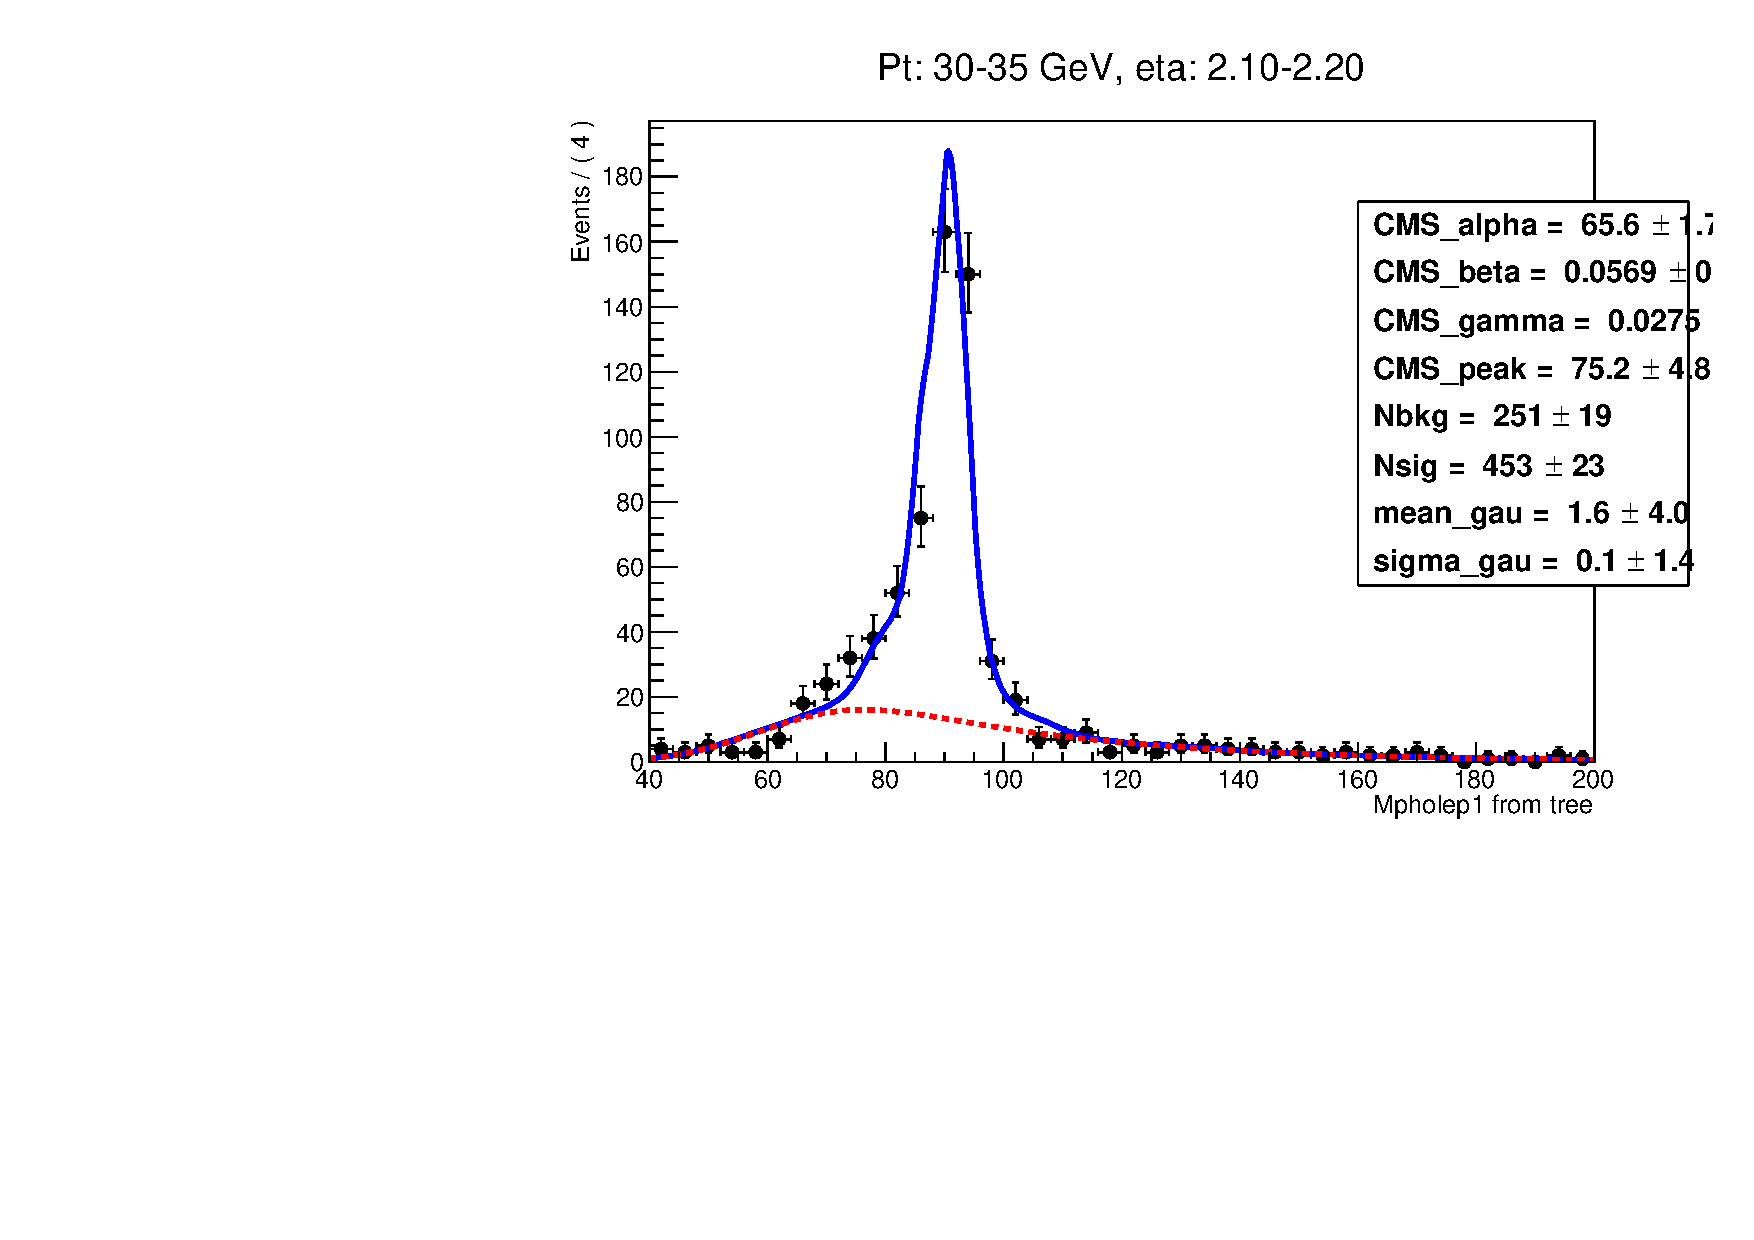
\includegraphics[width=0.45\textwidth]{../figs/figs_v11/ELECTRON_WGamma/EtoGammaFits/sa_hZmass_h_Data_EtoGamma_Enr_ENDCAP_pt30to35_ieta1.pdf}\\
   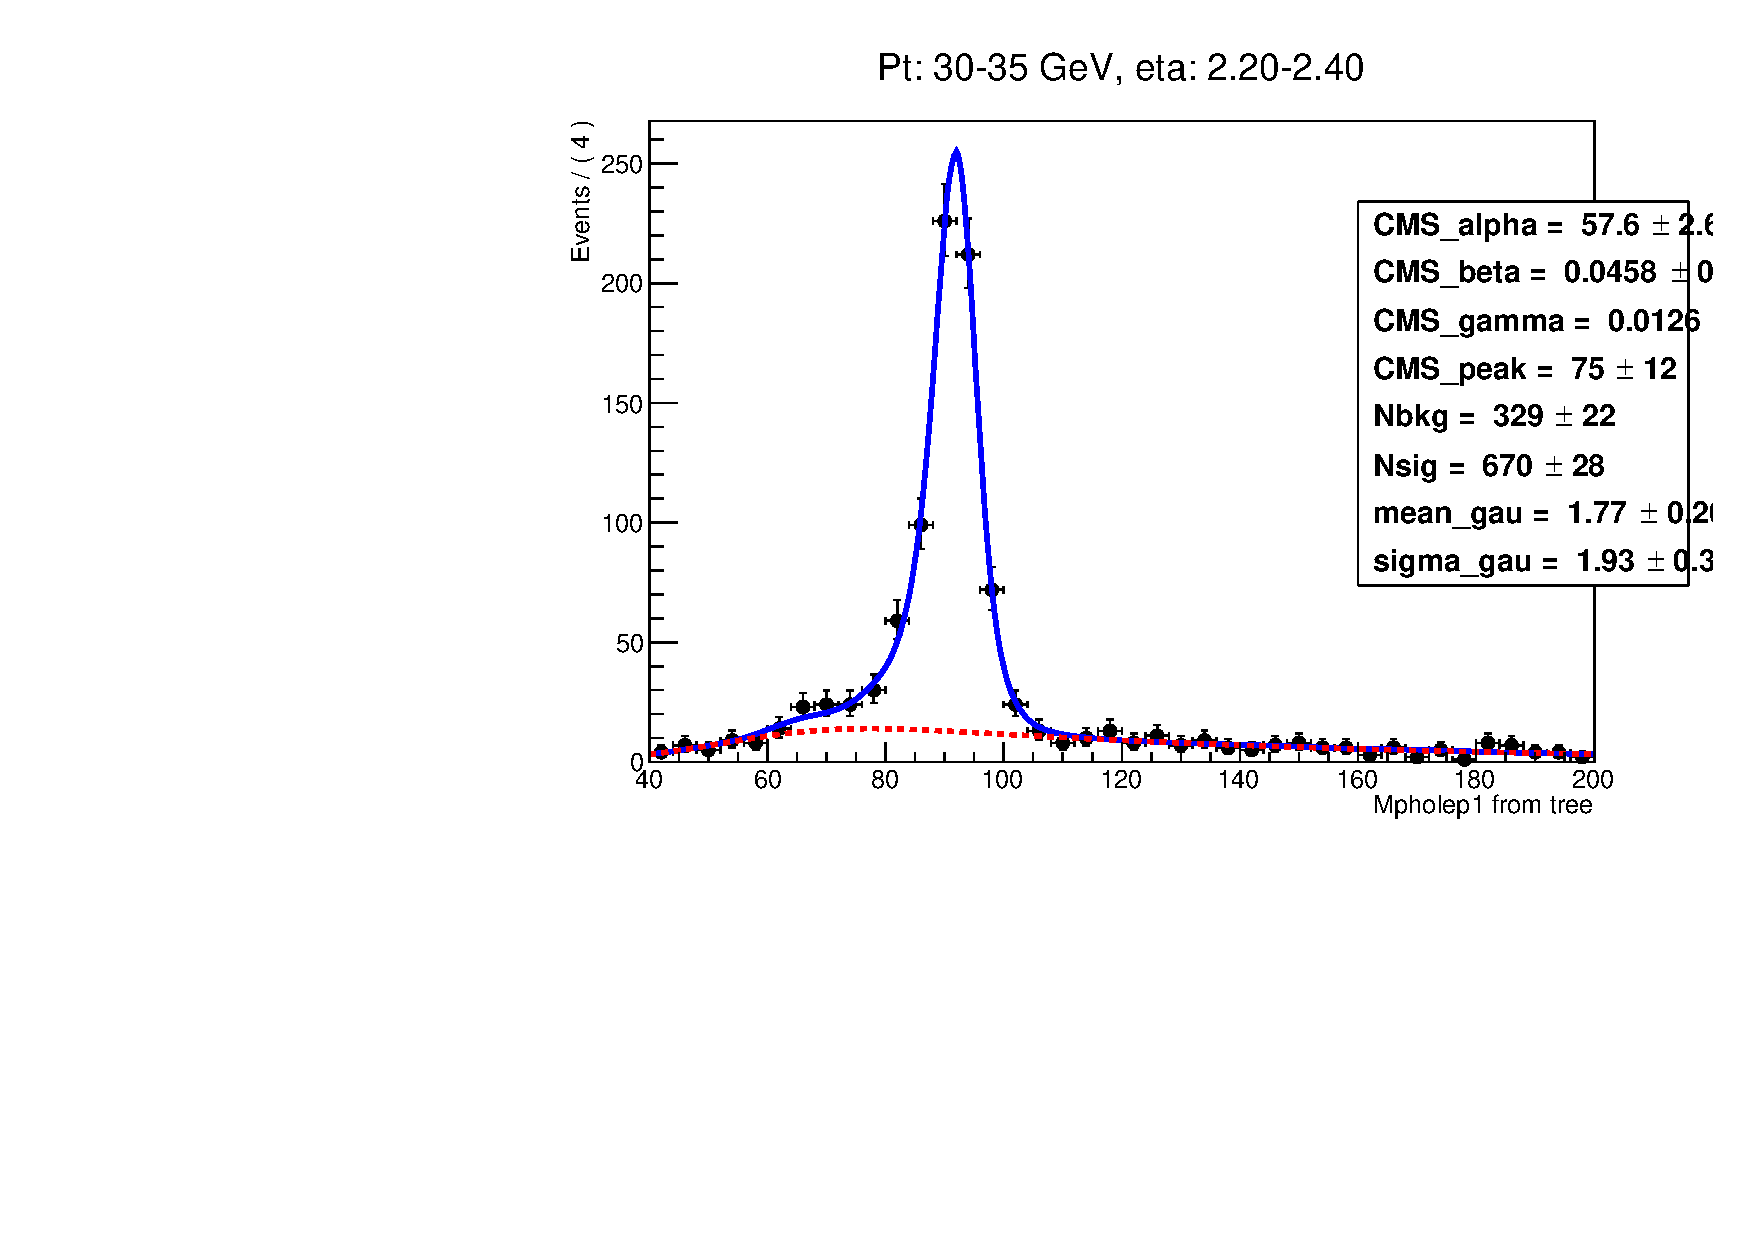
\includegraphics[width=0.45\textwidth]{../figs/figs_v11/ELECTRON_WGamma/EtoGammaFits/sa_hZmass_h_Data_EtoGamma_Enr_ENDCAP_pt30to35_ieta2.pdf}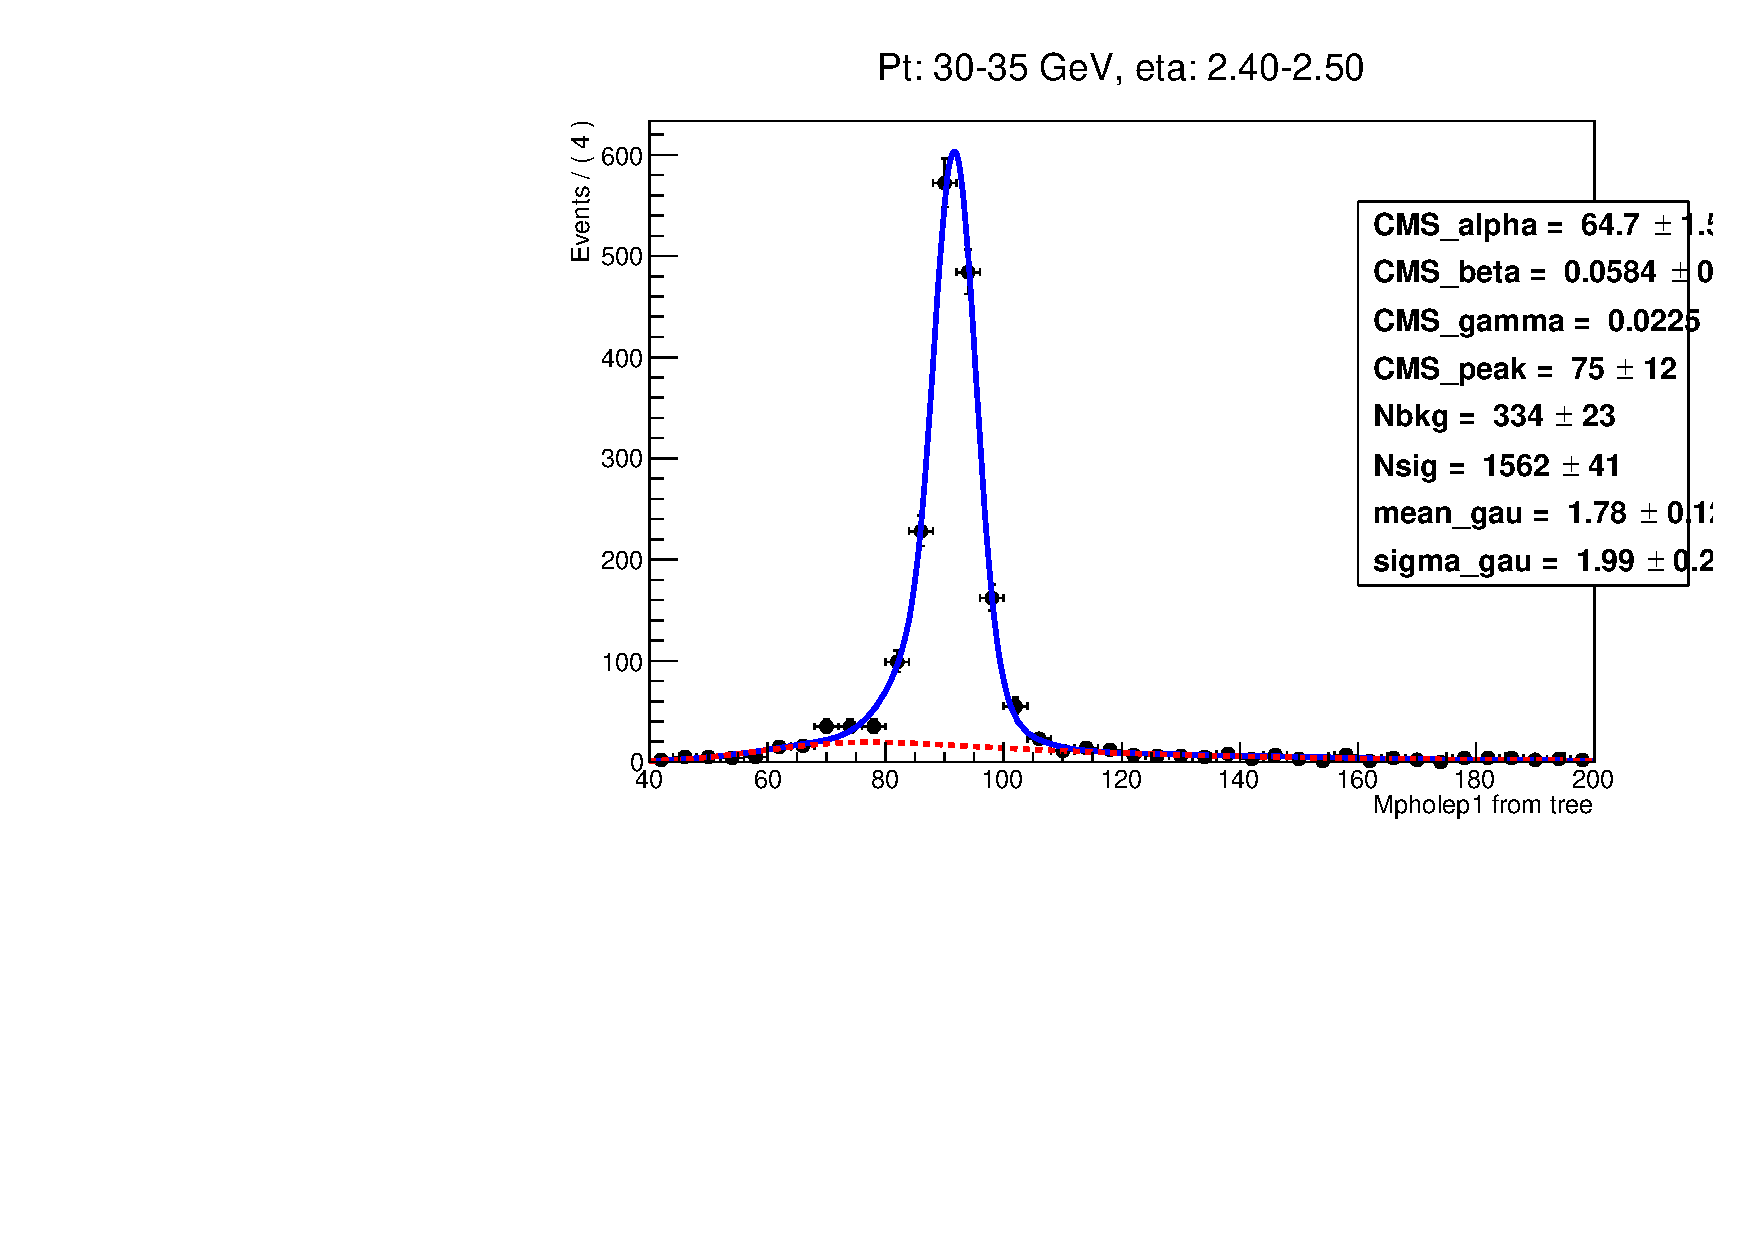
\includegraphics[width=0.45\textwidth]{../figs/figs_v11/ELECTRON_WGamma/EtoGammaFits/sa_hZmass_h_Data_EtoGamma_Enr_ENDCAP_pt30to35_ieta3.pdf}\\
  \label{fig:etogFits_30to35}
  \caption{$M_{e\gamma}$ fits, $W\gamma$, electron channel, 30-35 GeV, 8 $\eta^{\gamma}$ bins.}
  \end{center}
\end{figure}

\begin{figure}[htb]
  \begin{center}
   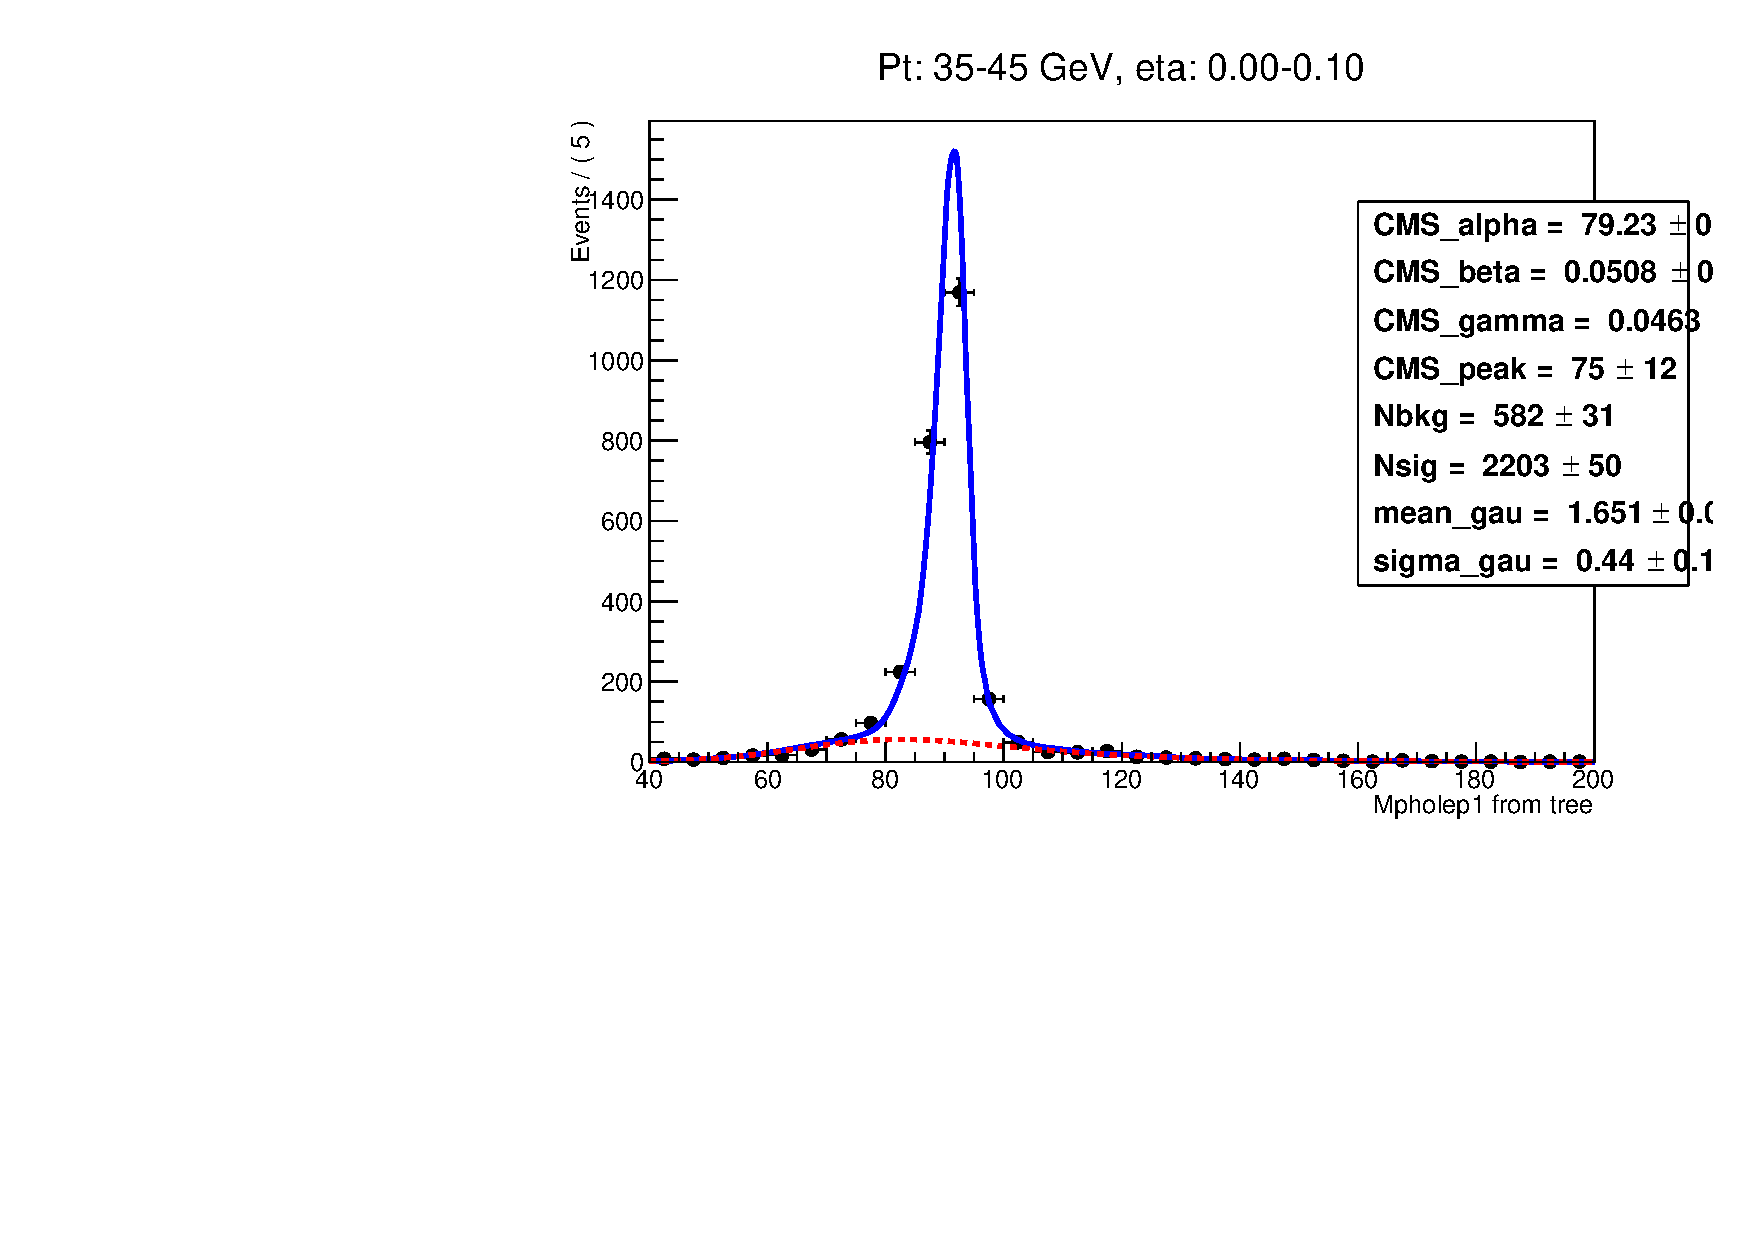
\includegraphics[width=0.45\textwidth]{../figs/figs_v11/ELECTRON_WGamma/EtoGammaFits/sa_hZmass_h_Data_EtoGamma_Enr_BARREL_pt35to45_ieta0.pdf}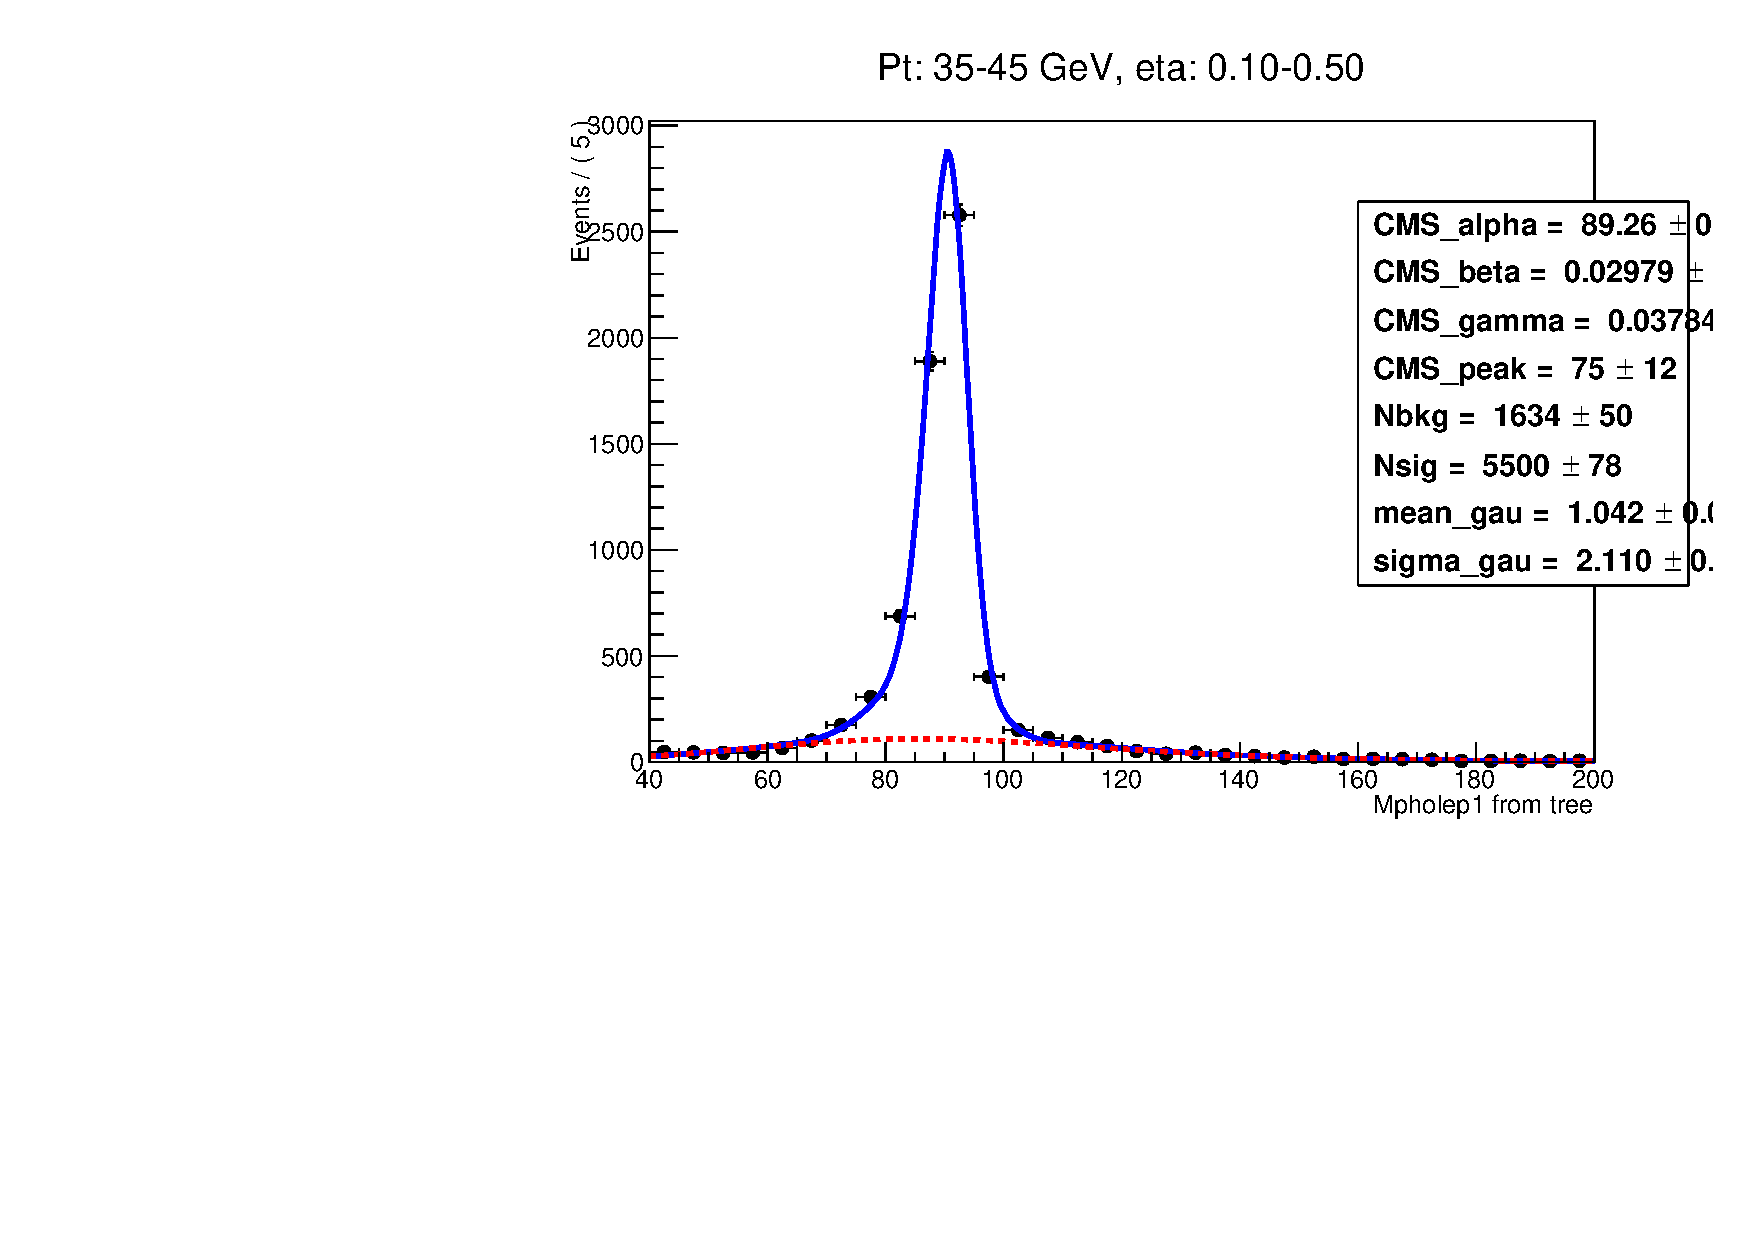
\includegraphics[width=0.45\textwidth]{../figs/figs_v11/ELECTRON_WGamma/EtoGammaFits/sa_hZmass_h_Data_EtoGamma_Enr_BARREL_pt35to45_ieta1.pdf}\\
   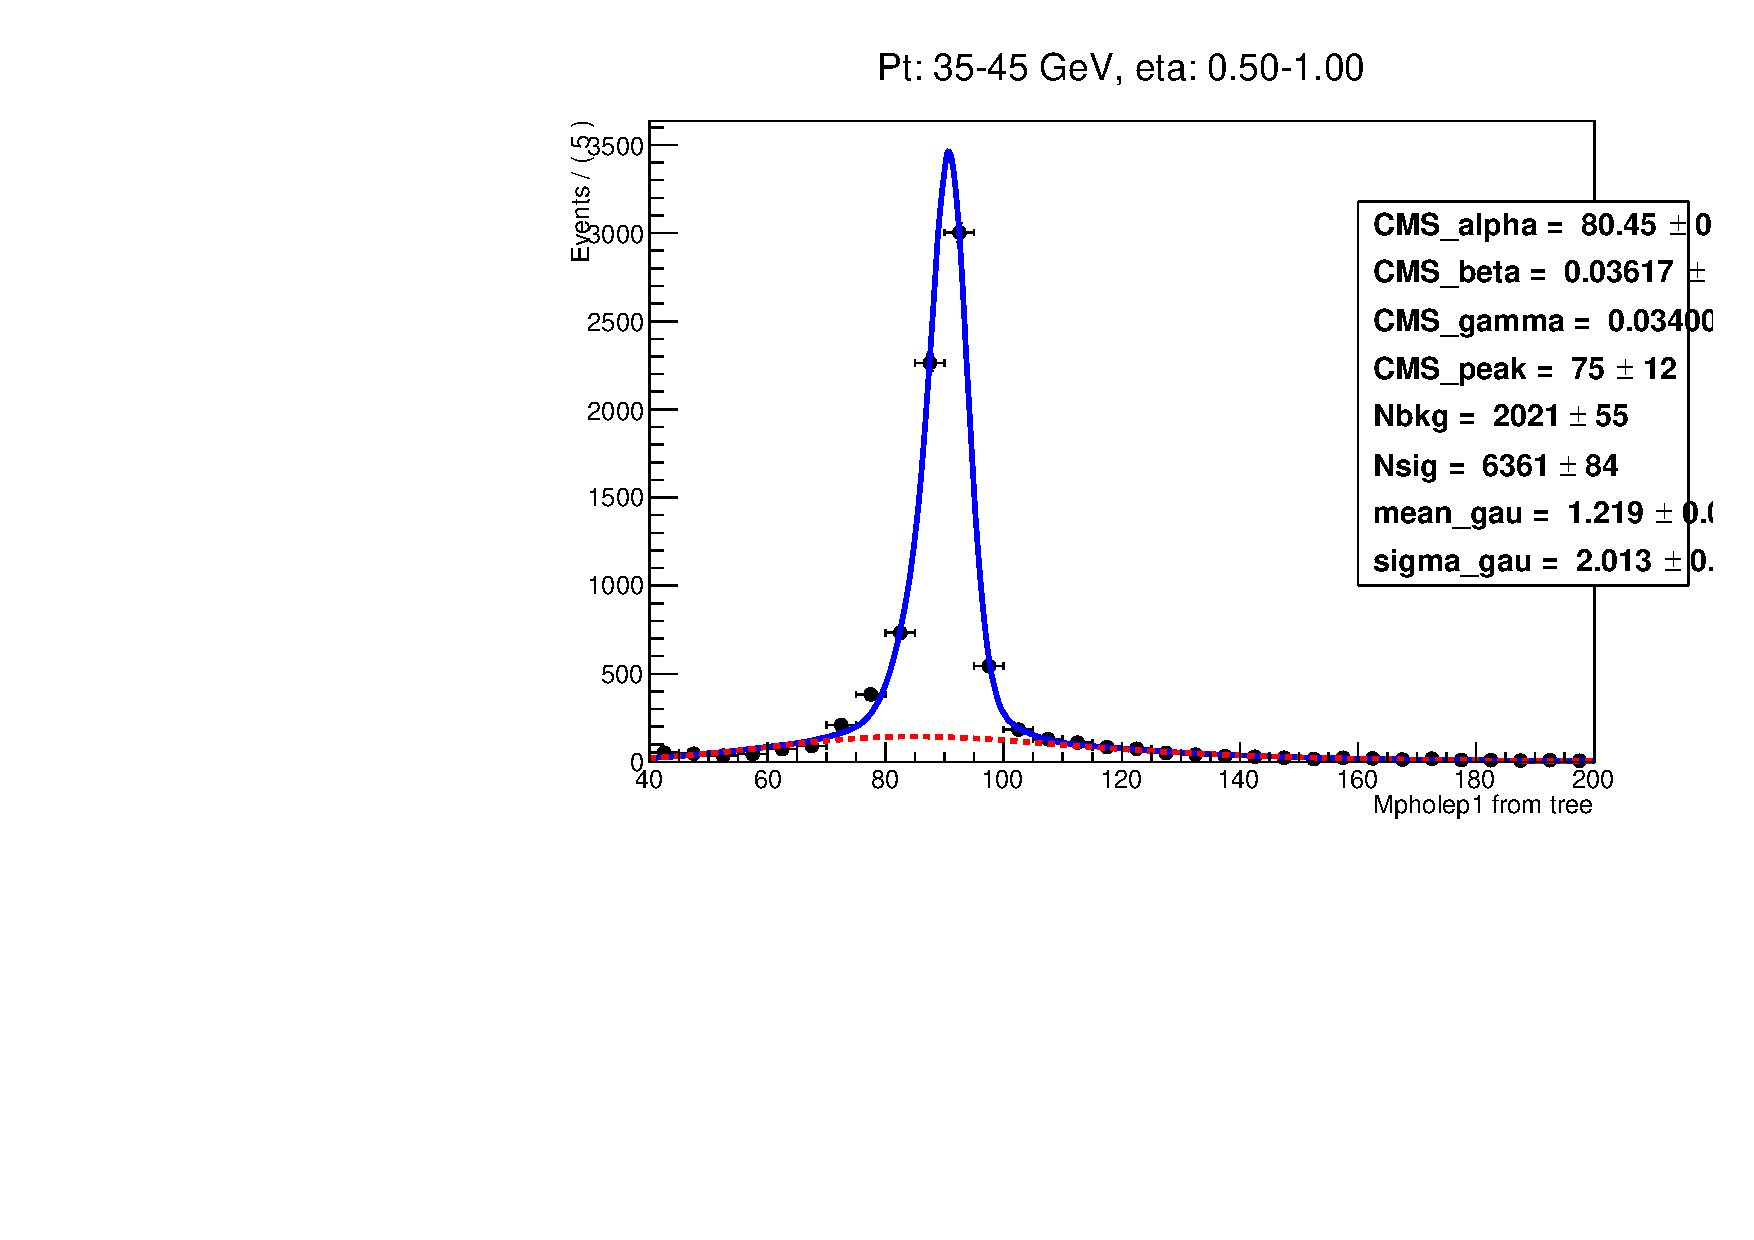
\includegraphics[width=0.45\textwidth]{../figs/figs_v11/ELECTRON_WGamma/EtoGammaFits/sa_hZmass_h_Data_EtoGamma_Enr_BARREL_pt35to45_ieta2.pdf}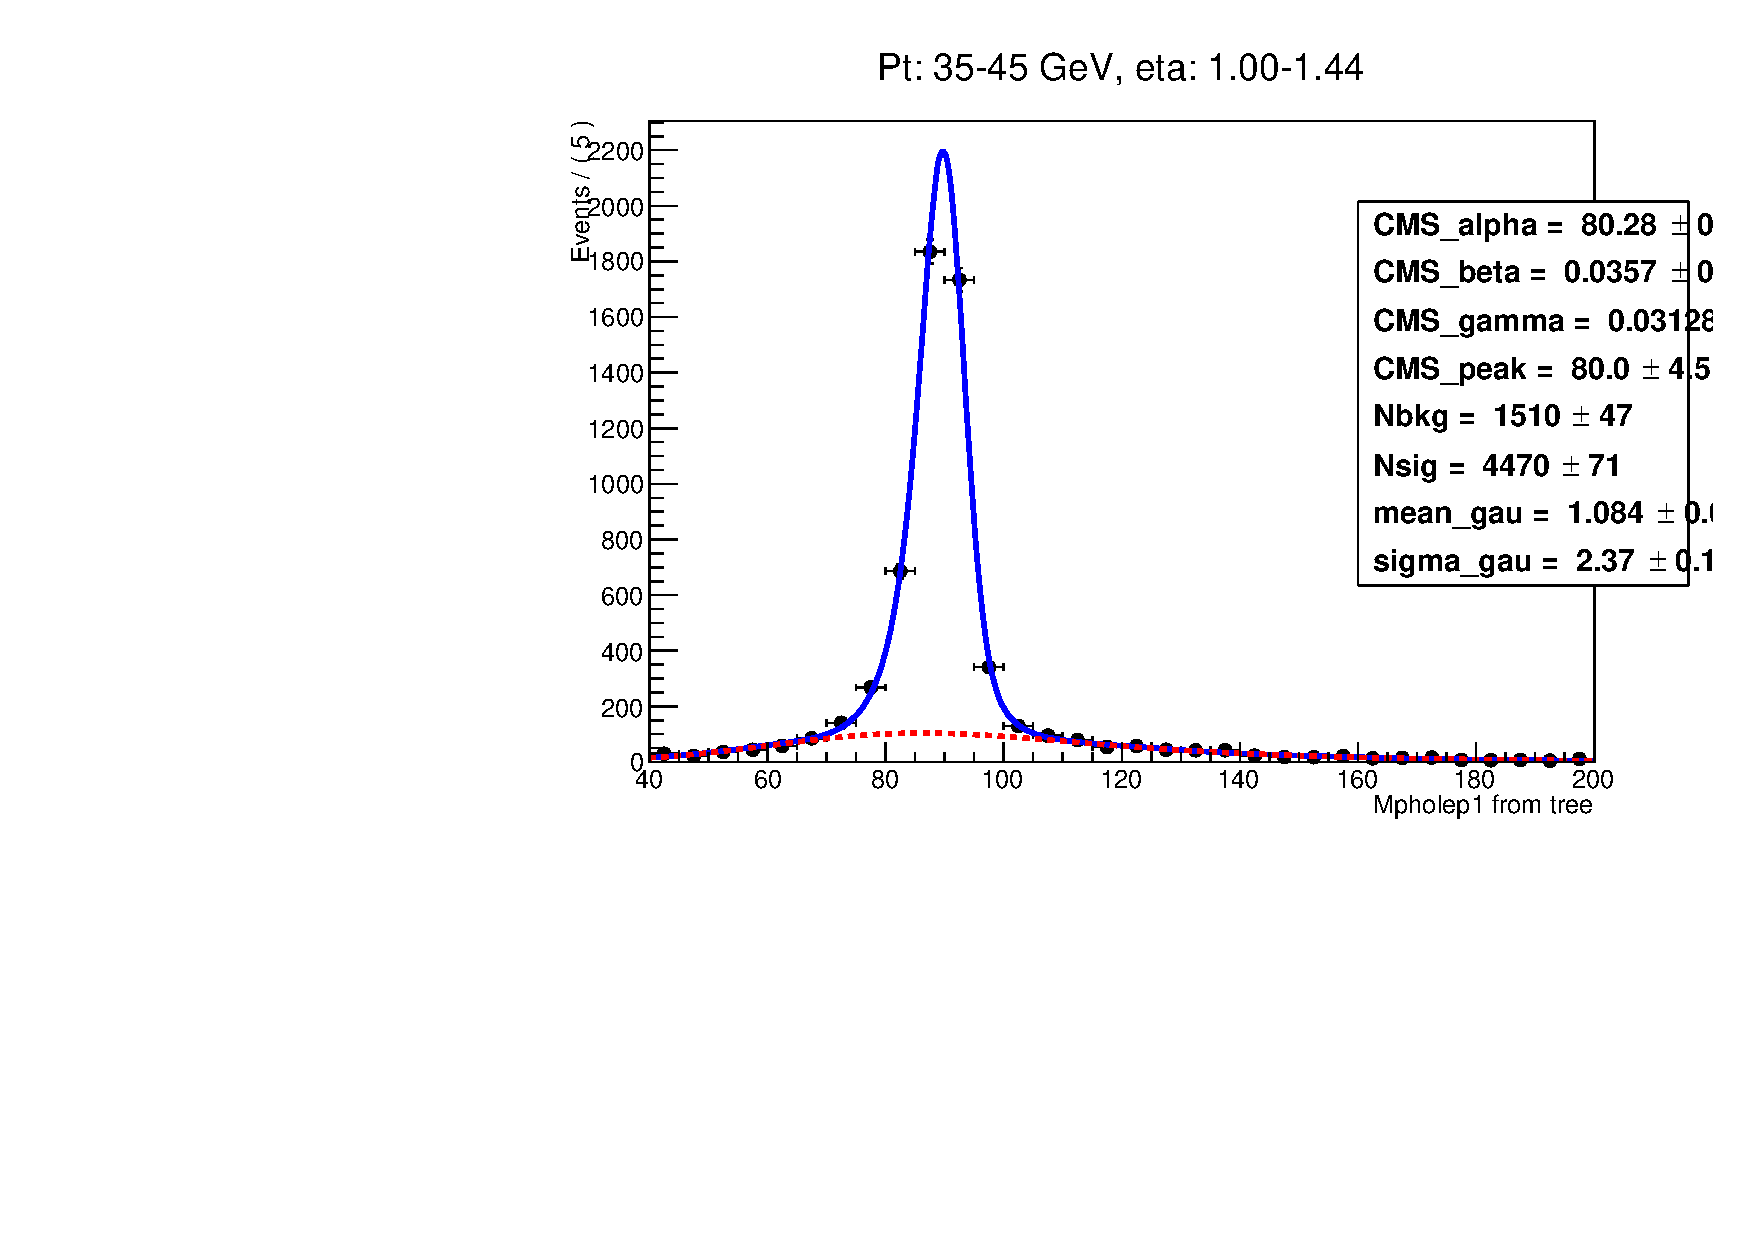
\includegraphics[width=0.45\textwidth]{../figs/figs_v11/ELECTRON_WGamma/EtoGammaFits/sa_hZmass_h_Data_EtoGamma_Enr_BARREL_pt35to45_ieta3.pdf}\\
   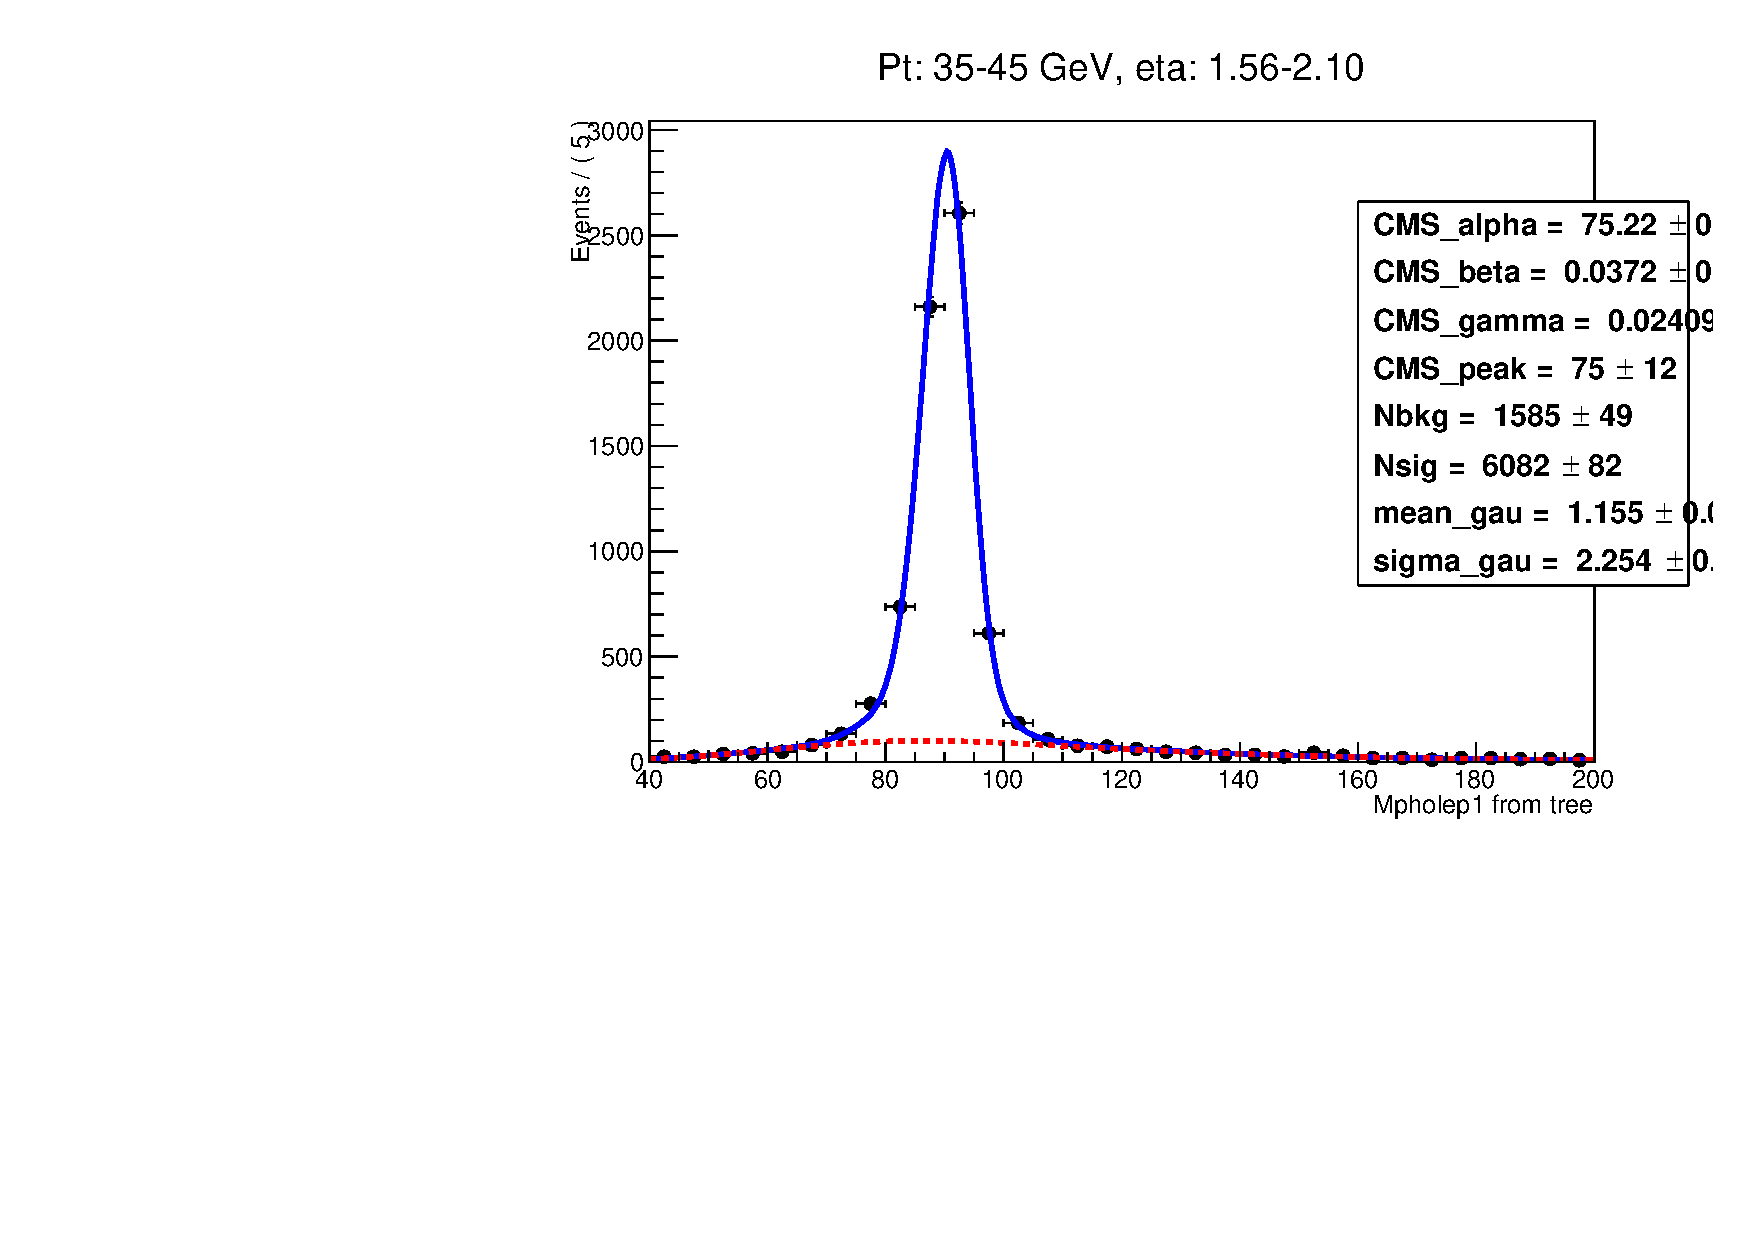
\includegraphics[width=0.45\textwidth]{../figs/figs_v11/ELECTRON_WGamma/EtoGammaFits/sa_hZmass_h_Data_EtoGamma_Enr_ENDCAP_pt35to45_ieta0.pdf}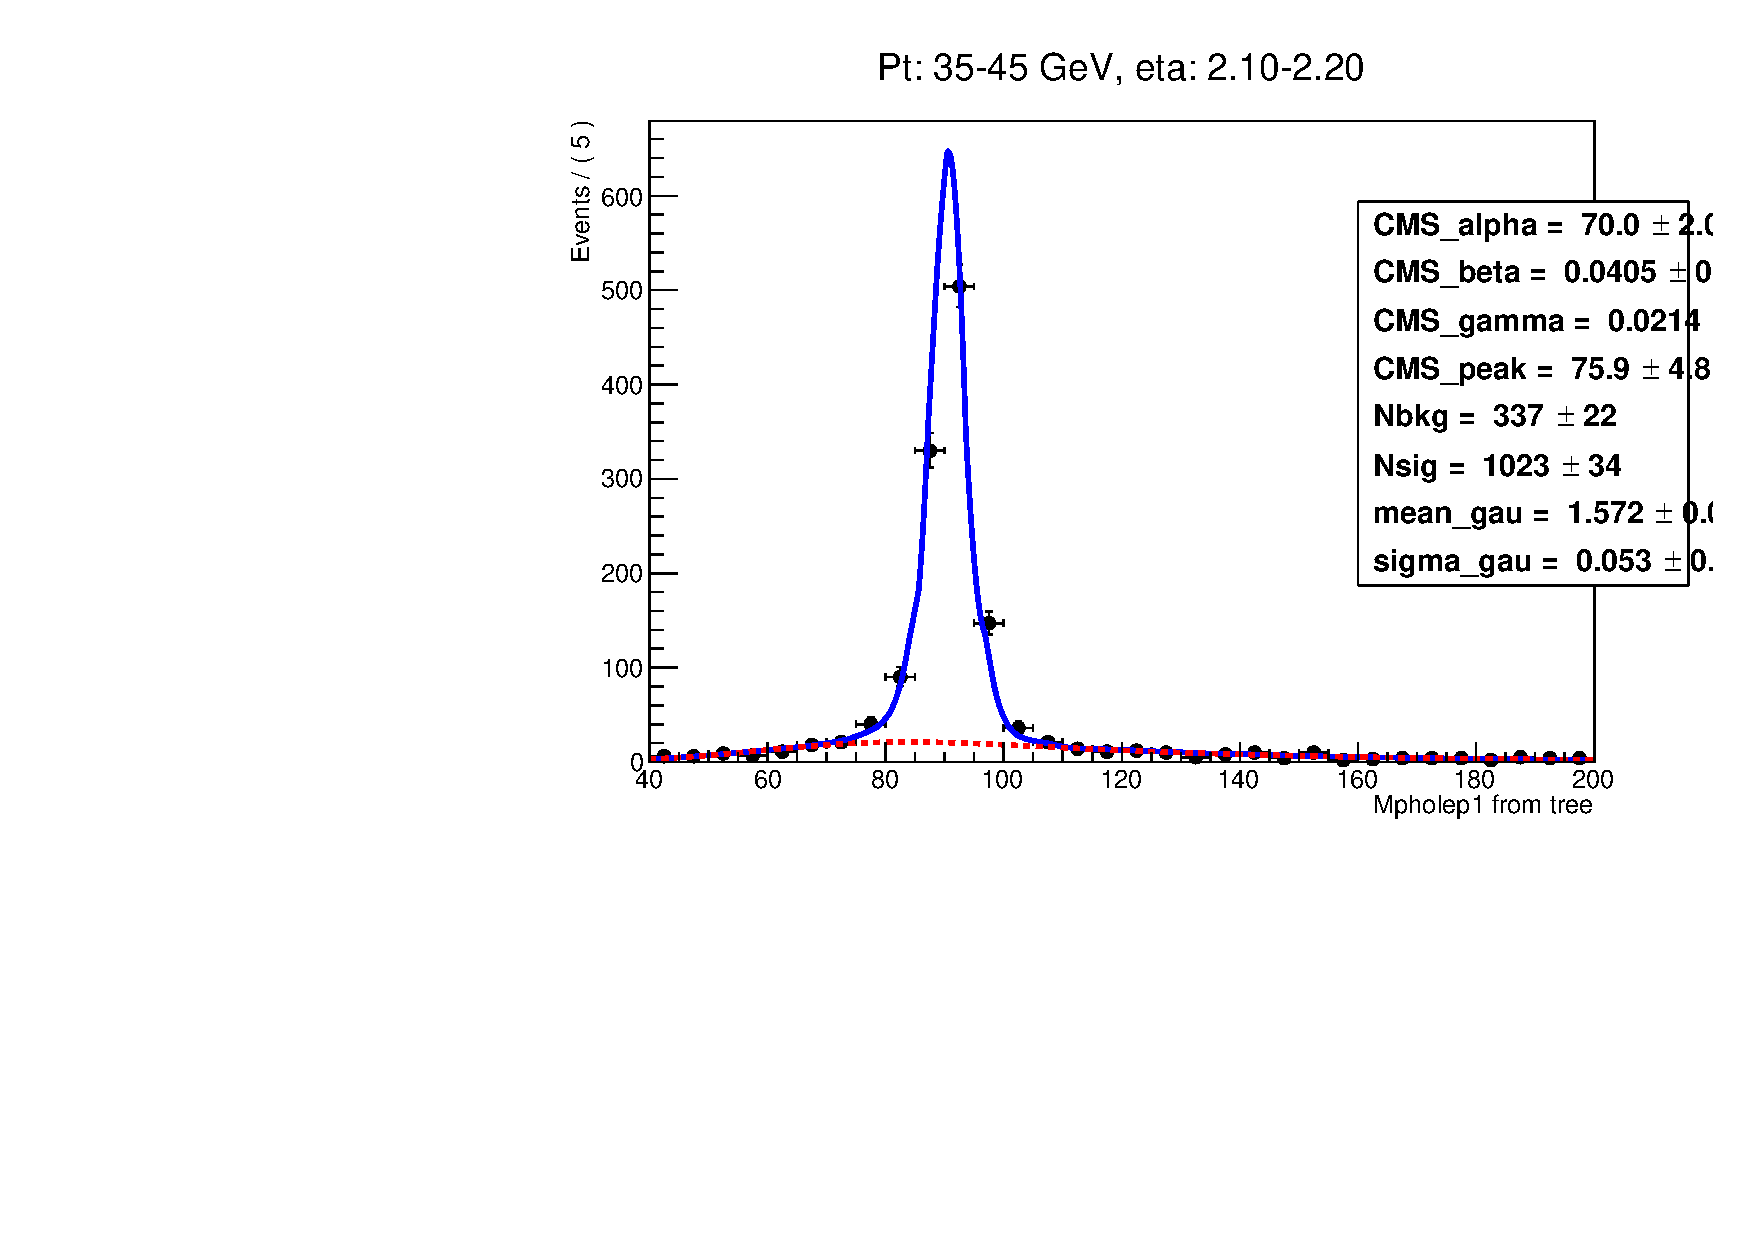
\includegraphics[width=0.45\textwidth]{../figs/figs_v11/ELECTRON_WGamma/EtoGammaFits/sa_hZmass_h_Data_EtoGamma_Enr_ENDCAP_pt35to45_ieta1.pdf}\\
   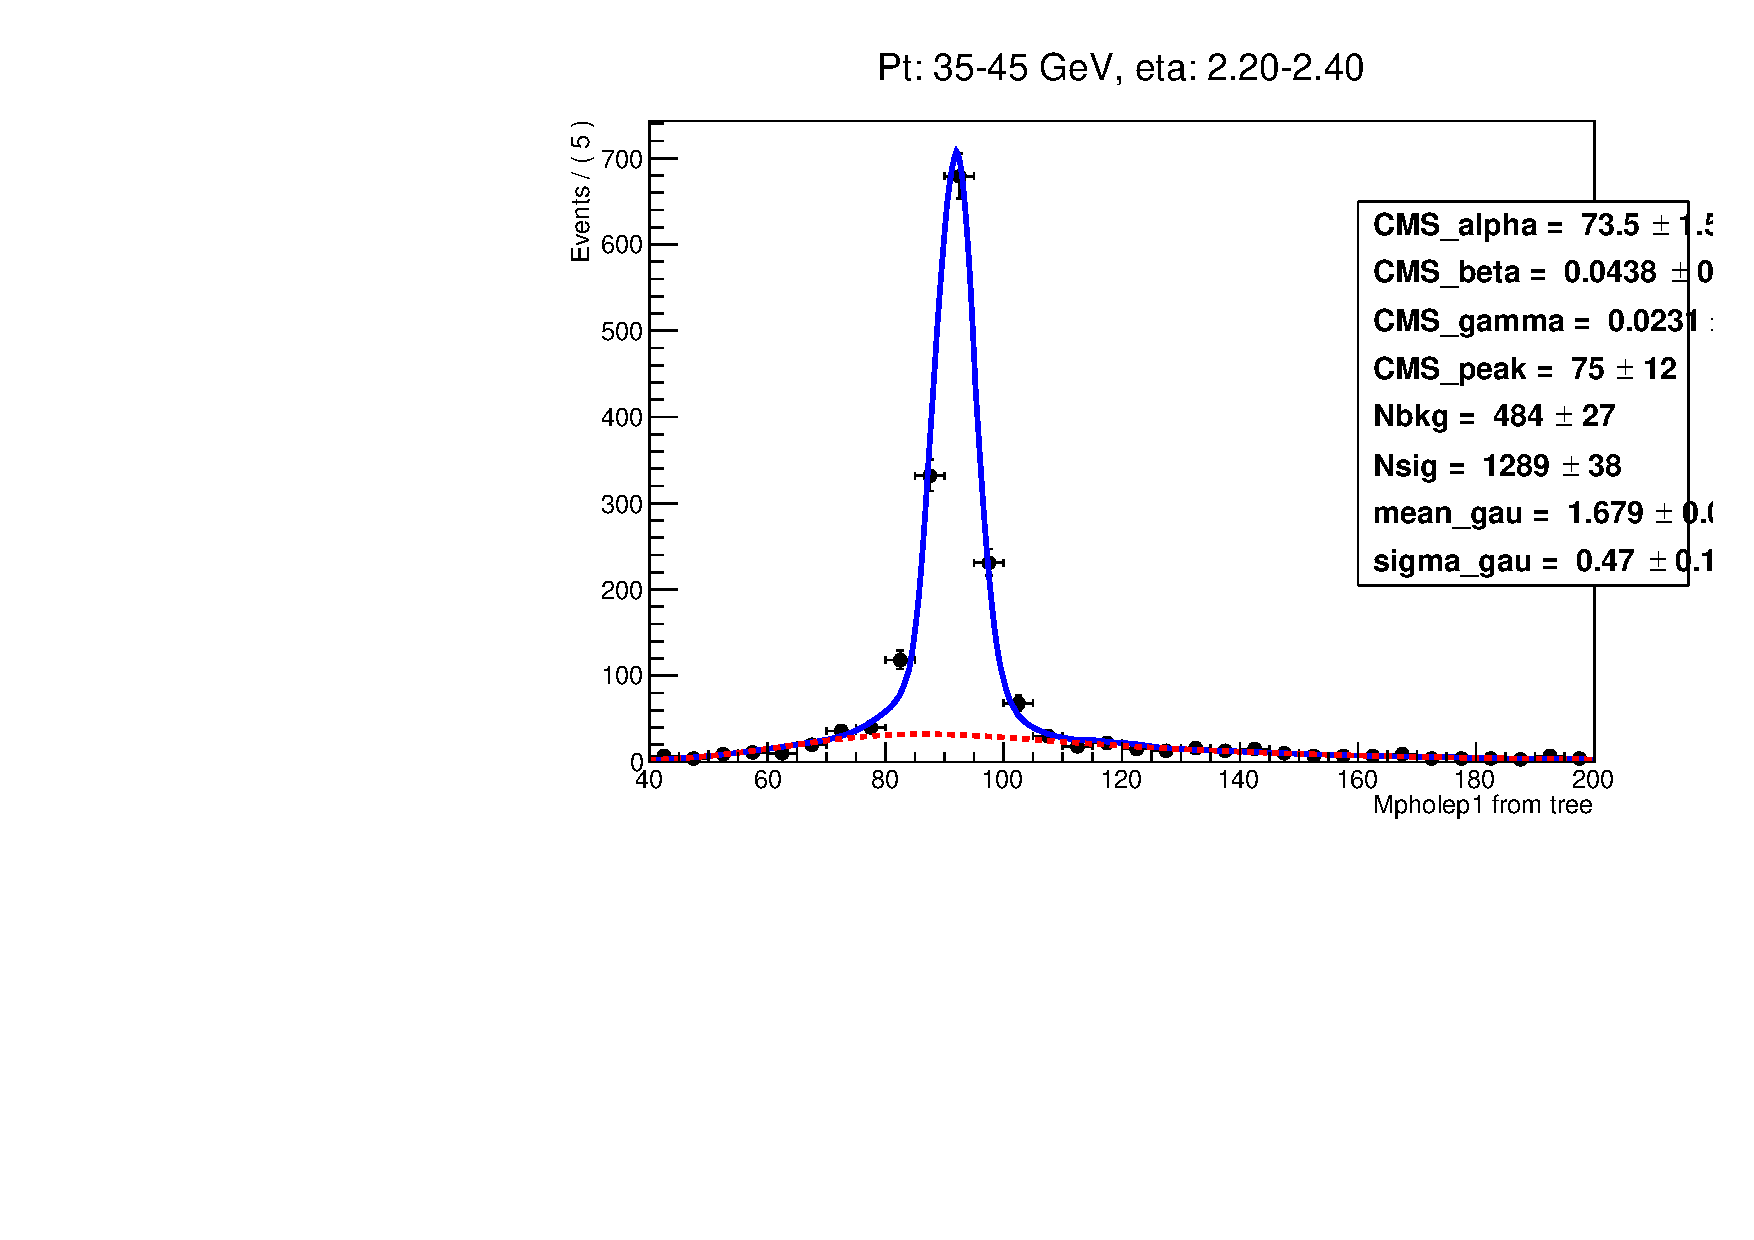
\includegraphics[width=0.45\textwidth]{../figs/figs_v11/ELECTRON_WGamma/EtoGammaFits/sa_hZmass_h_Data_EtoGamma_Enr_ENDCAP_pt35to45_ieta2.pdf}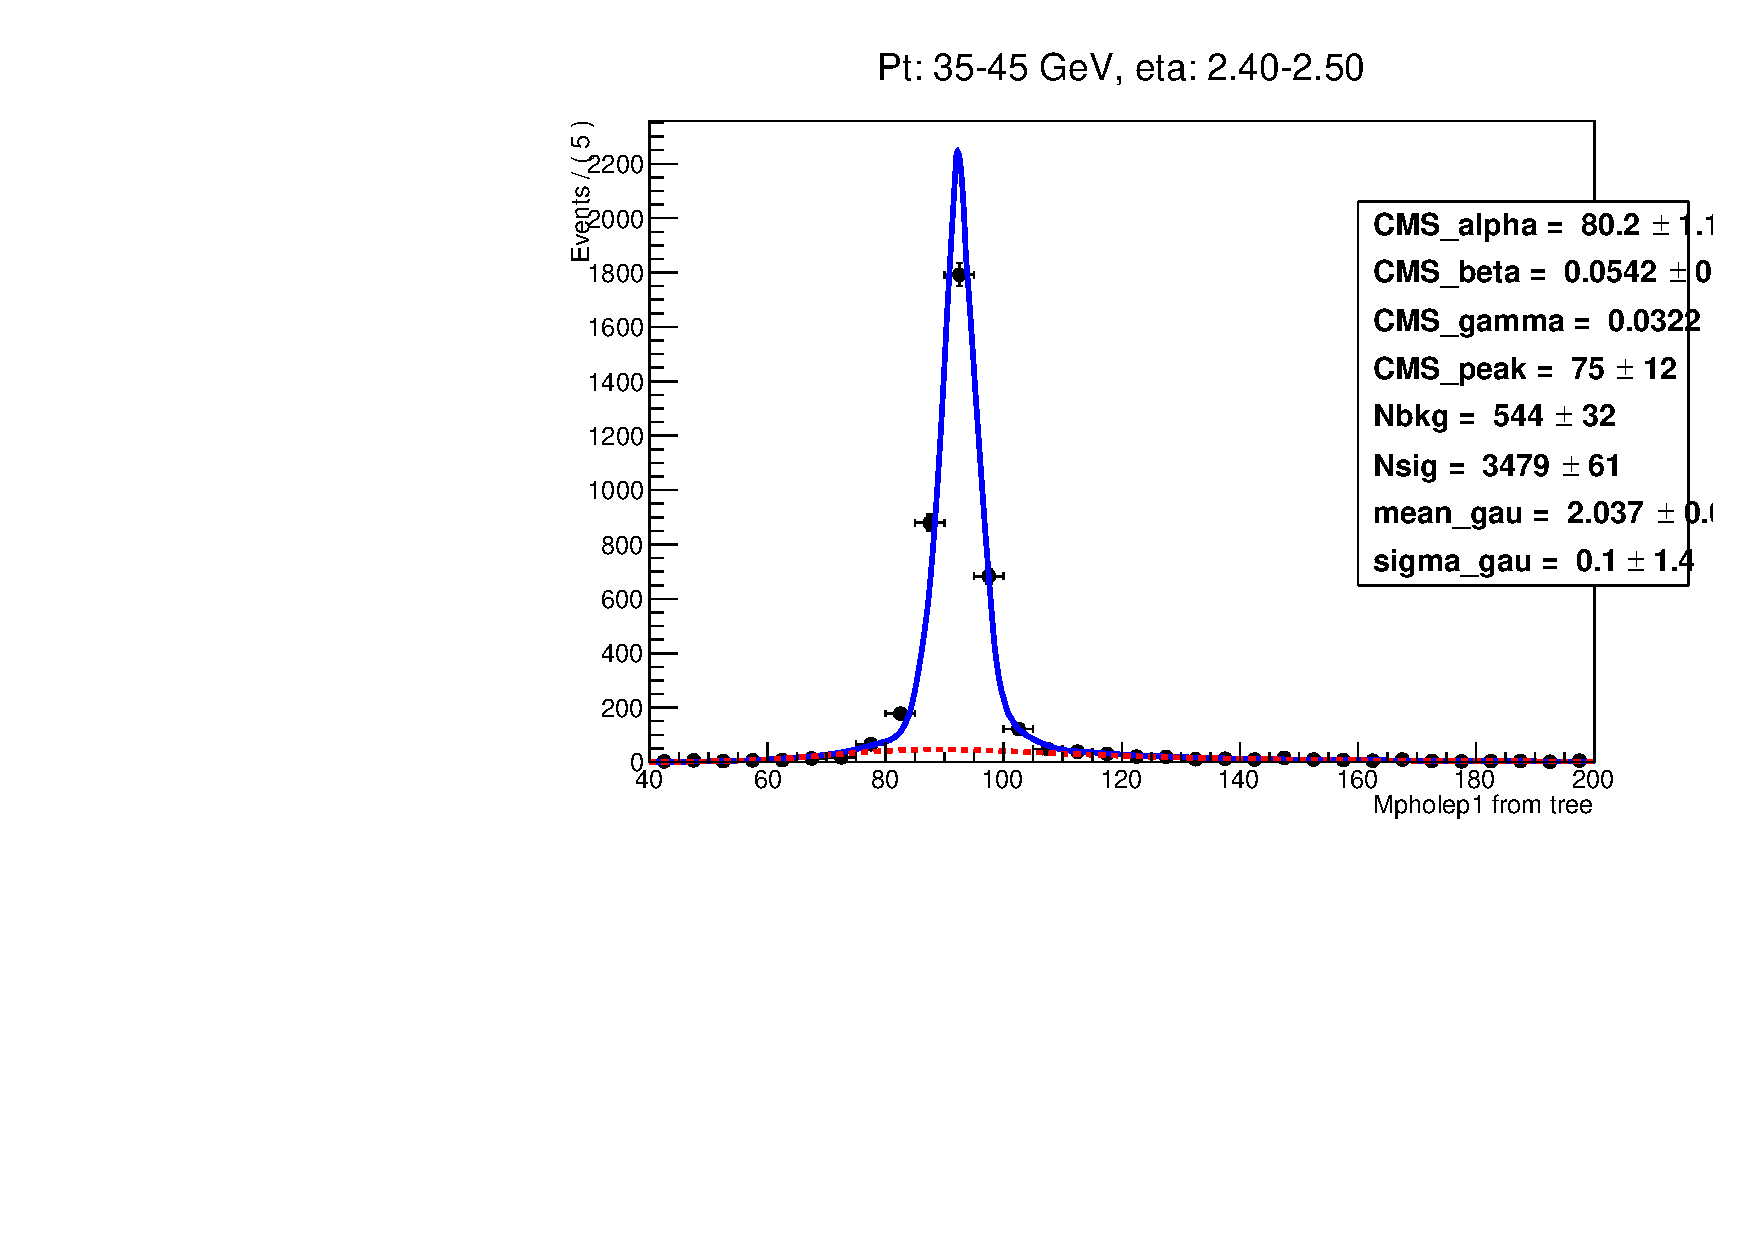
\includegraphics[width=0.45\textwidth]{../figs/figs_v11/ELECTRON_WGamma/EtoGammaFits/sa_hZmass_h_Data_EtoGamma_Enr_ENDCAP_pt35to45_ieta3.pdf}\\
  \label{fig:etogFits_35to45}
  \caption{$M_{e\gamma}$ fits, $W\gamma$, electron channel, 35-45 GeV, 8 $\eta^{\gamma}$ bins.}
  \end{center}
\end{figure}

\begin{figure}[htb]
  \begin{center}
   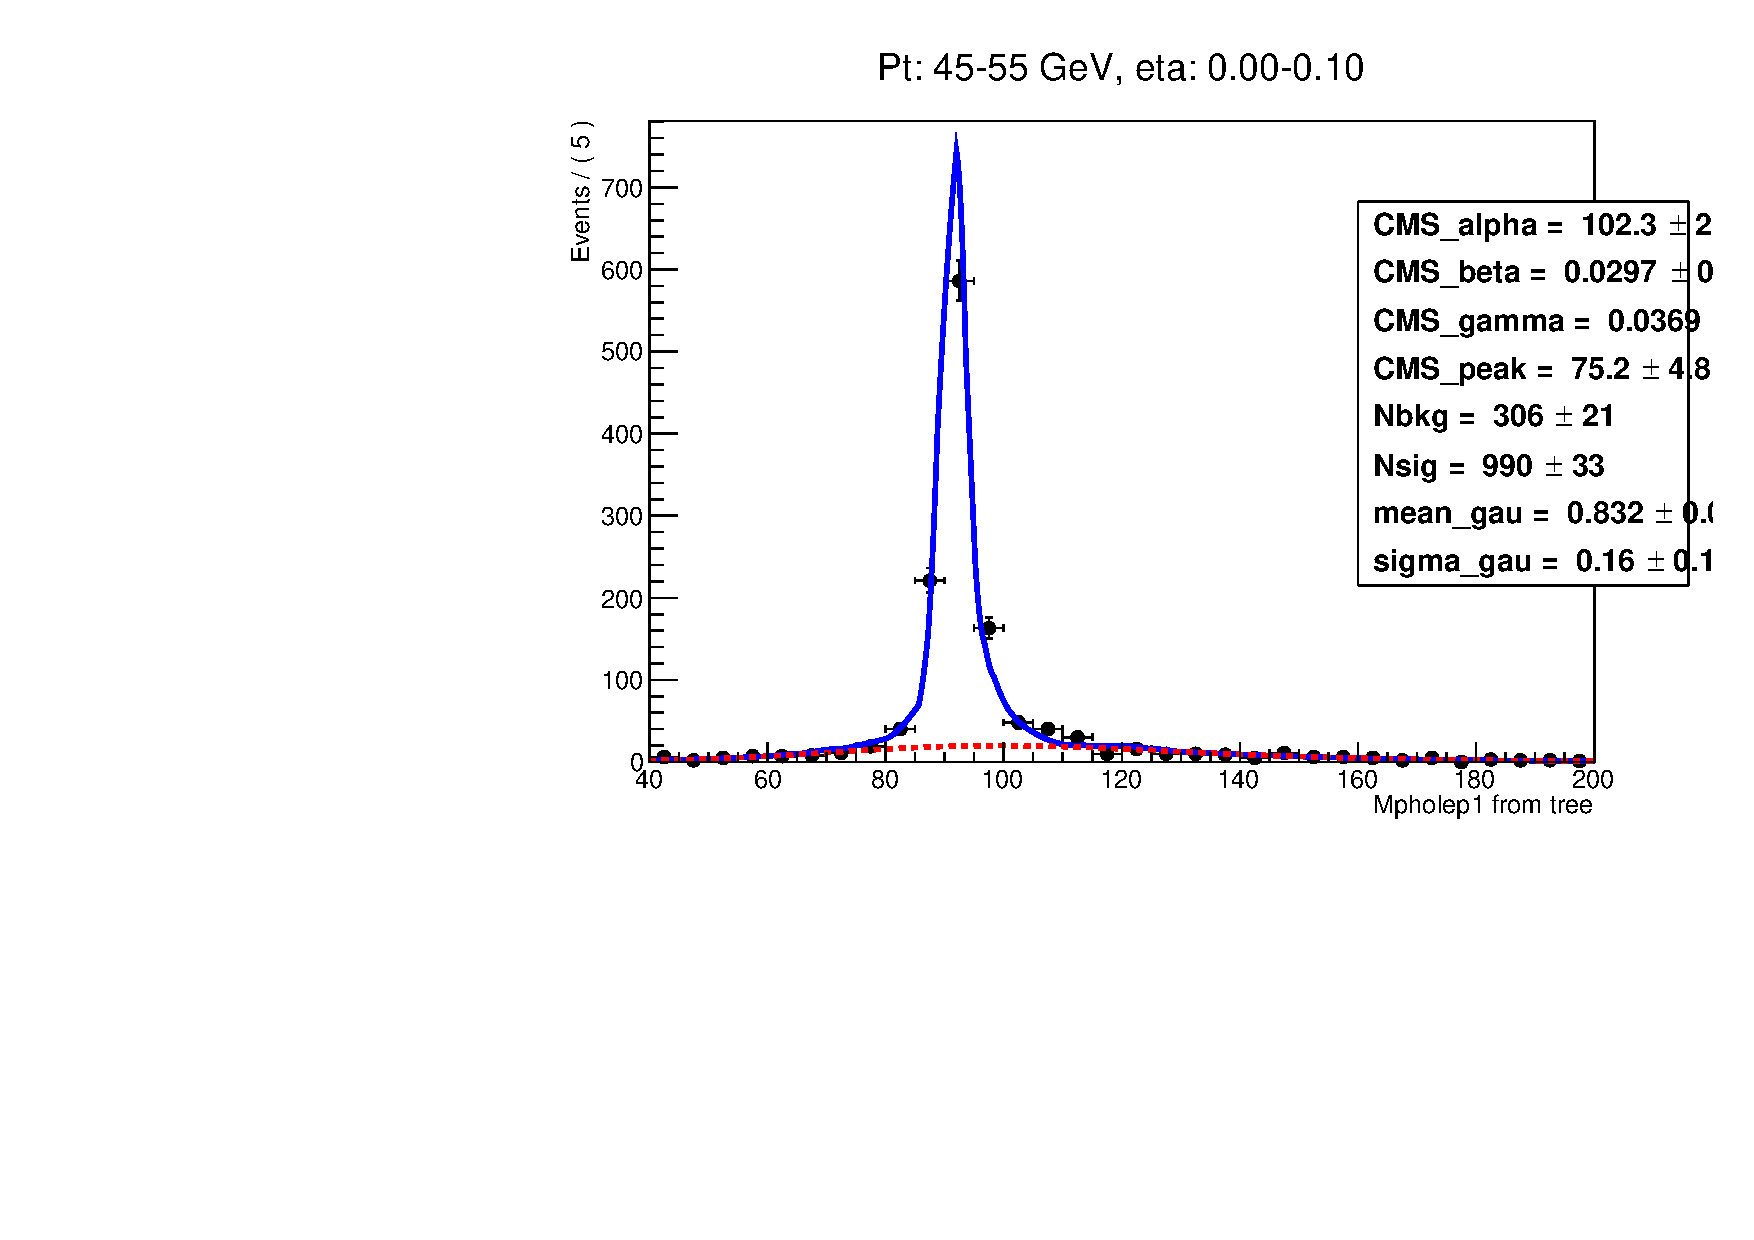
\includegraphics[width=0.45\textwidth]{../figs/figs_v11/ELECTRON_WGamma/EtoGammaFits/sa_hZmass_h_Data_EtoGamma_Enr_BARREL_pt45to55_ieta0.pdf}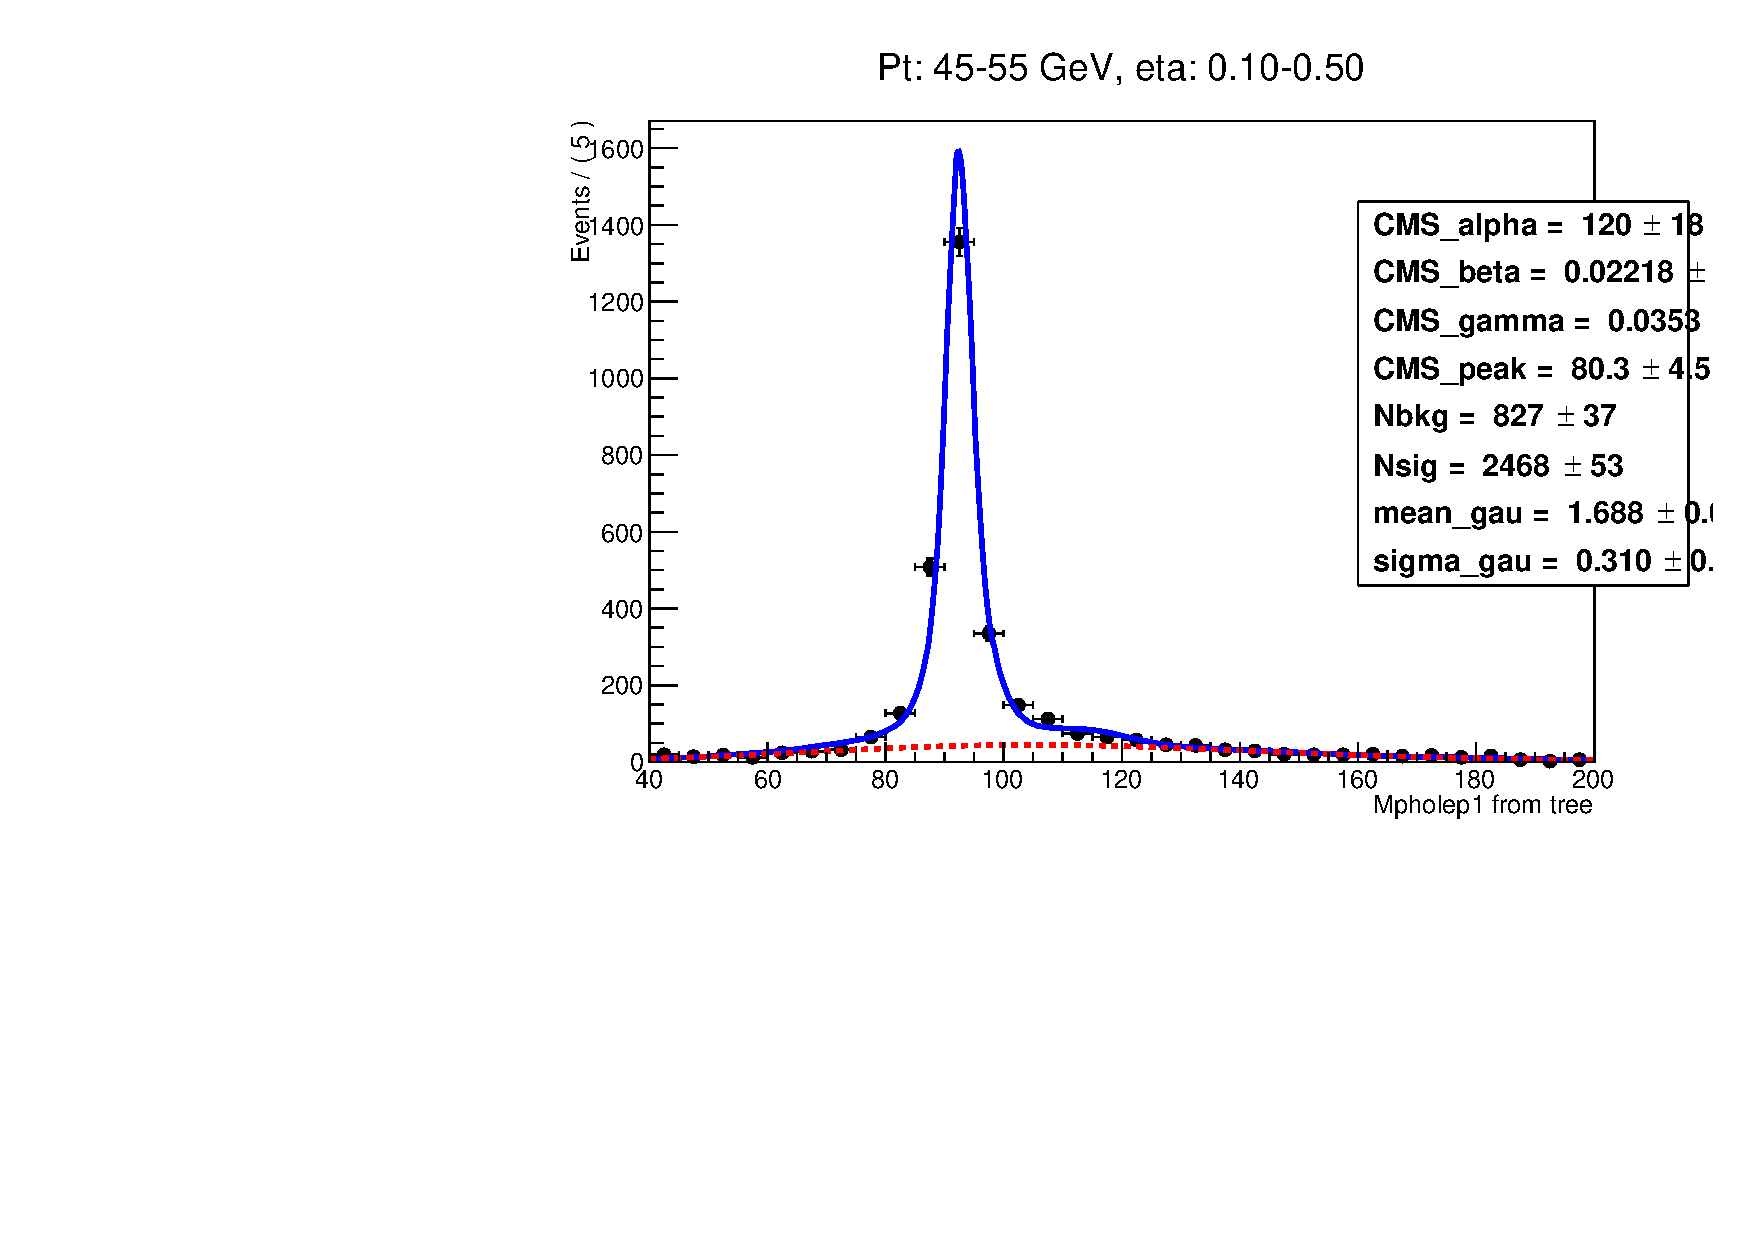
\includegraphics[width=0.45\textwidth]{../figs/figs_v11/ELECTRON_WGamma/EtoGammaFits/sa_hZmass_h_Data_EtoGamma_Enr_BARREL_pt45to55_ieta1.pdf}\\
   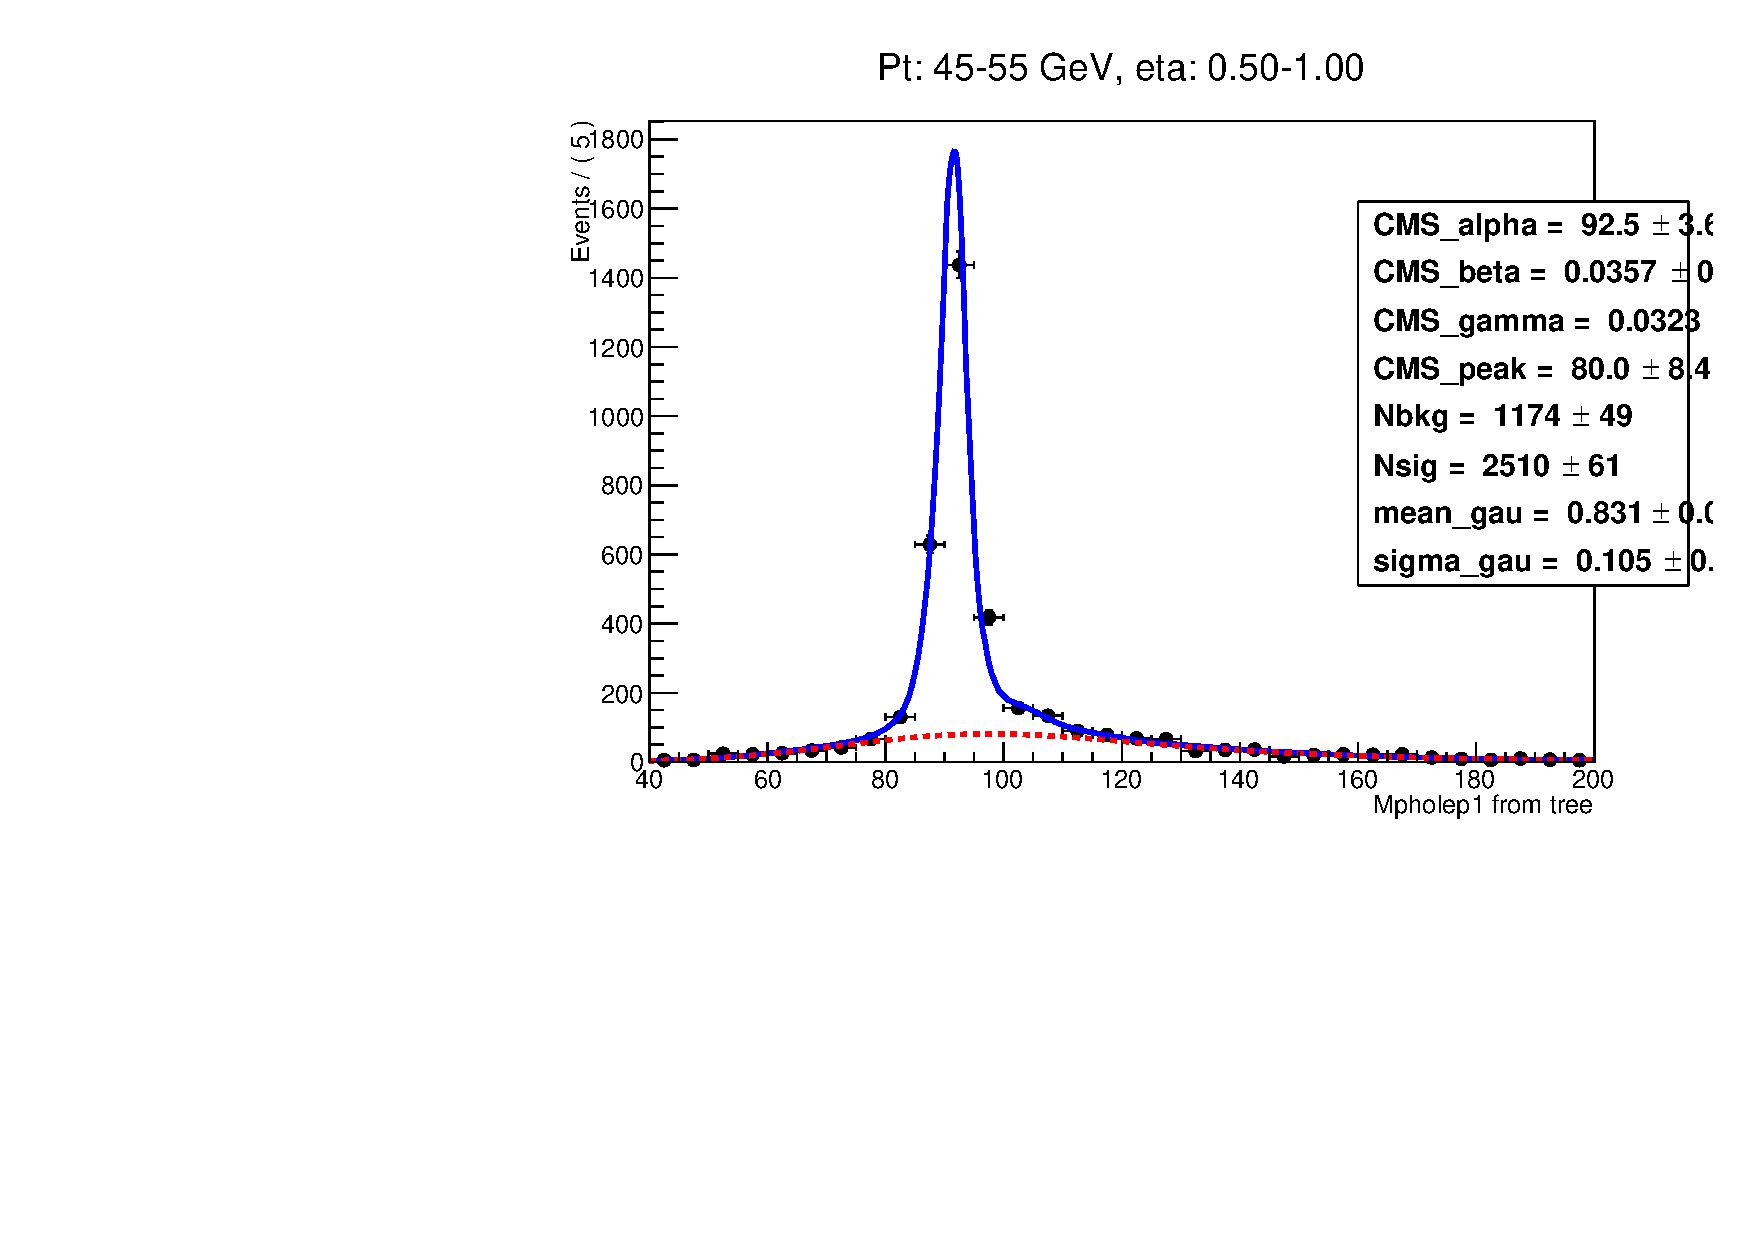
\includegraphics[width=0.45\textwidth]{../figs/figs_v11/ELECTRON_WGamma/EtoGammaFits/sa_hZmass_h_Data_EtoGamma_Enr_BARREL_pt45to55_ieta2.pdf}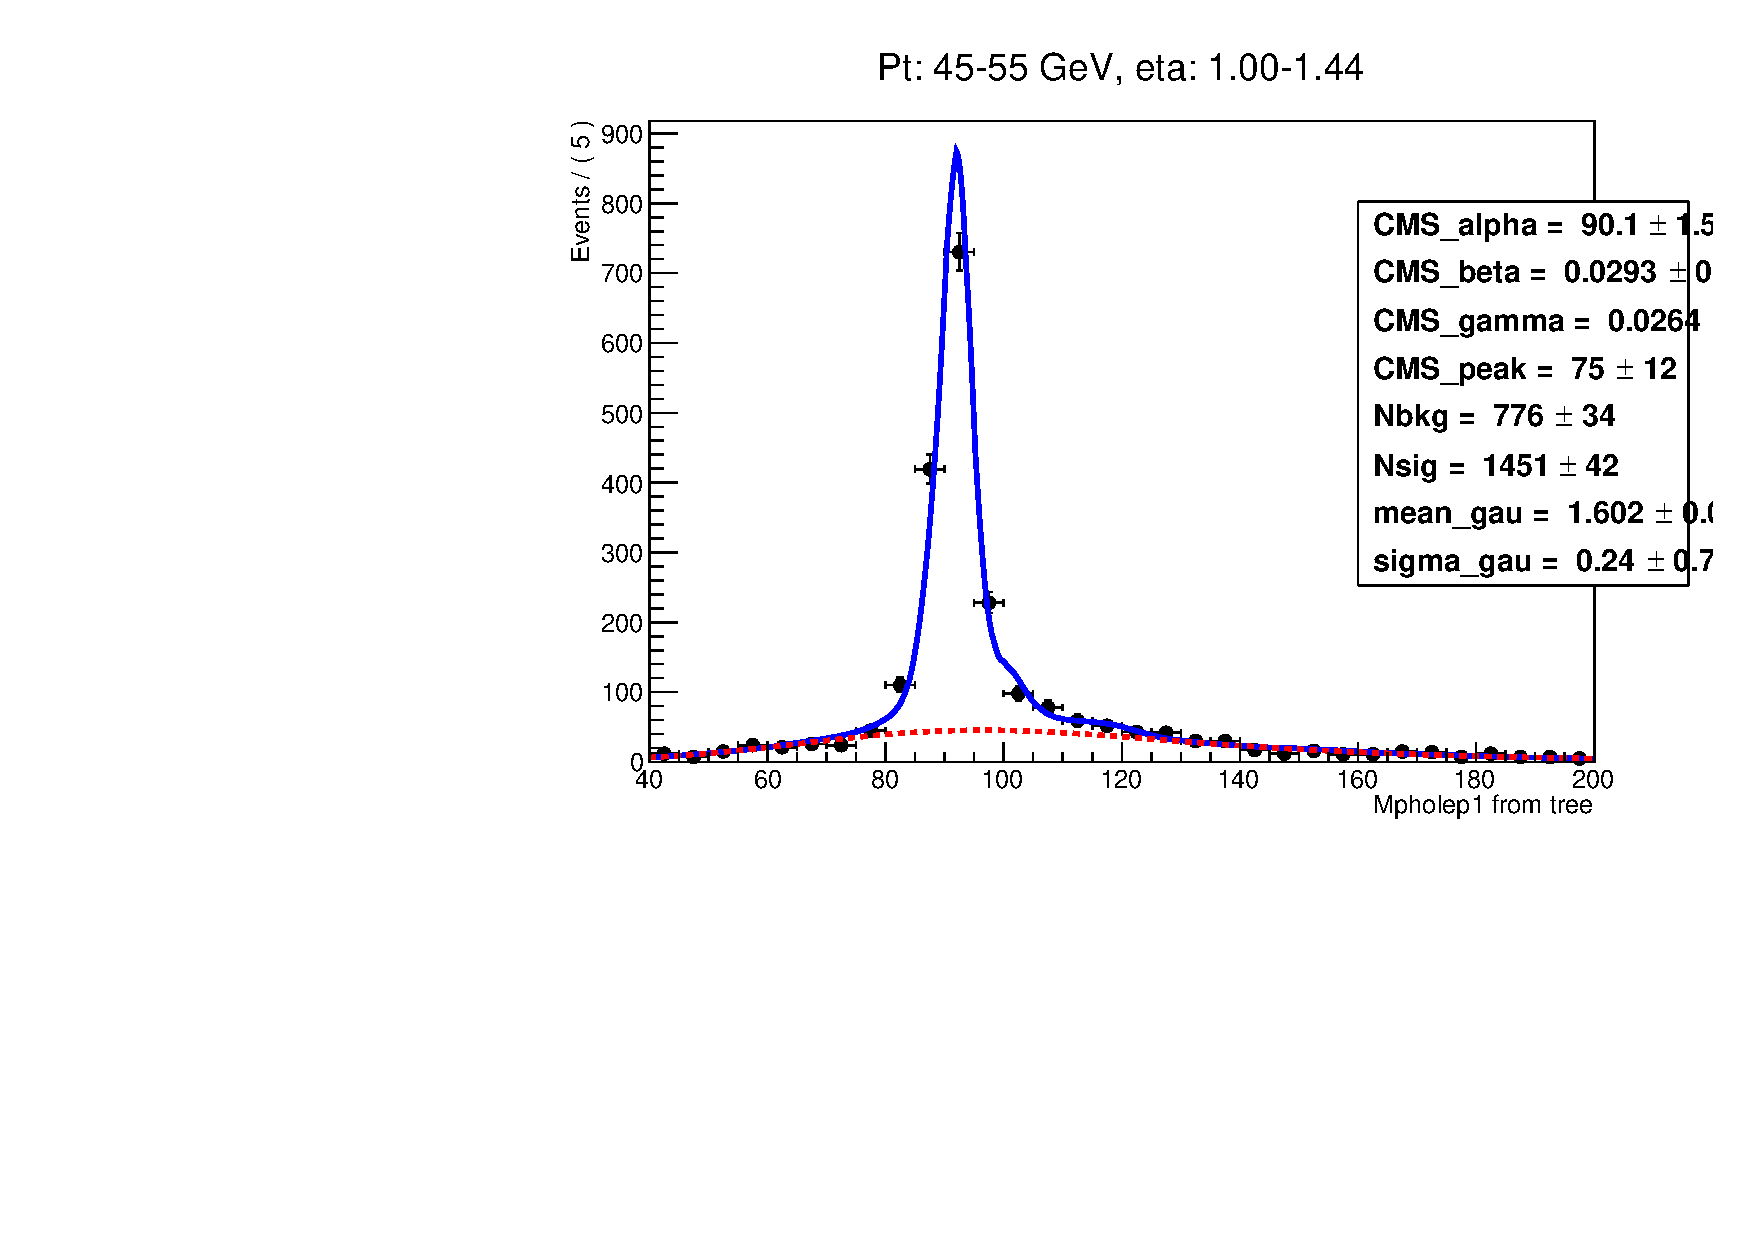
\includegraphics[width=0.45\textwidth]{../figs/figs_v11/ELECTRON_WGamma/EtoGammaFits/sa_hZmass_h_Data_EtoGamma_Enr_BARREL_pt45to55_ieta3.pdf}\\
   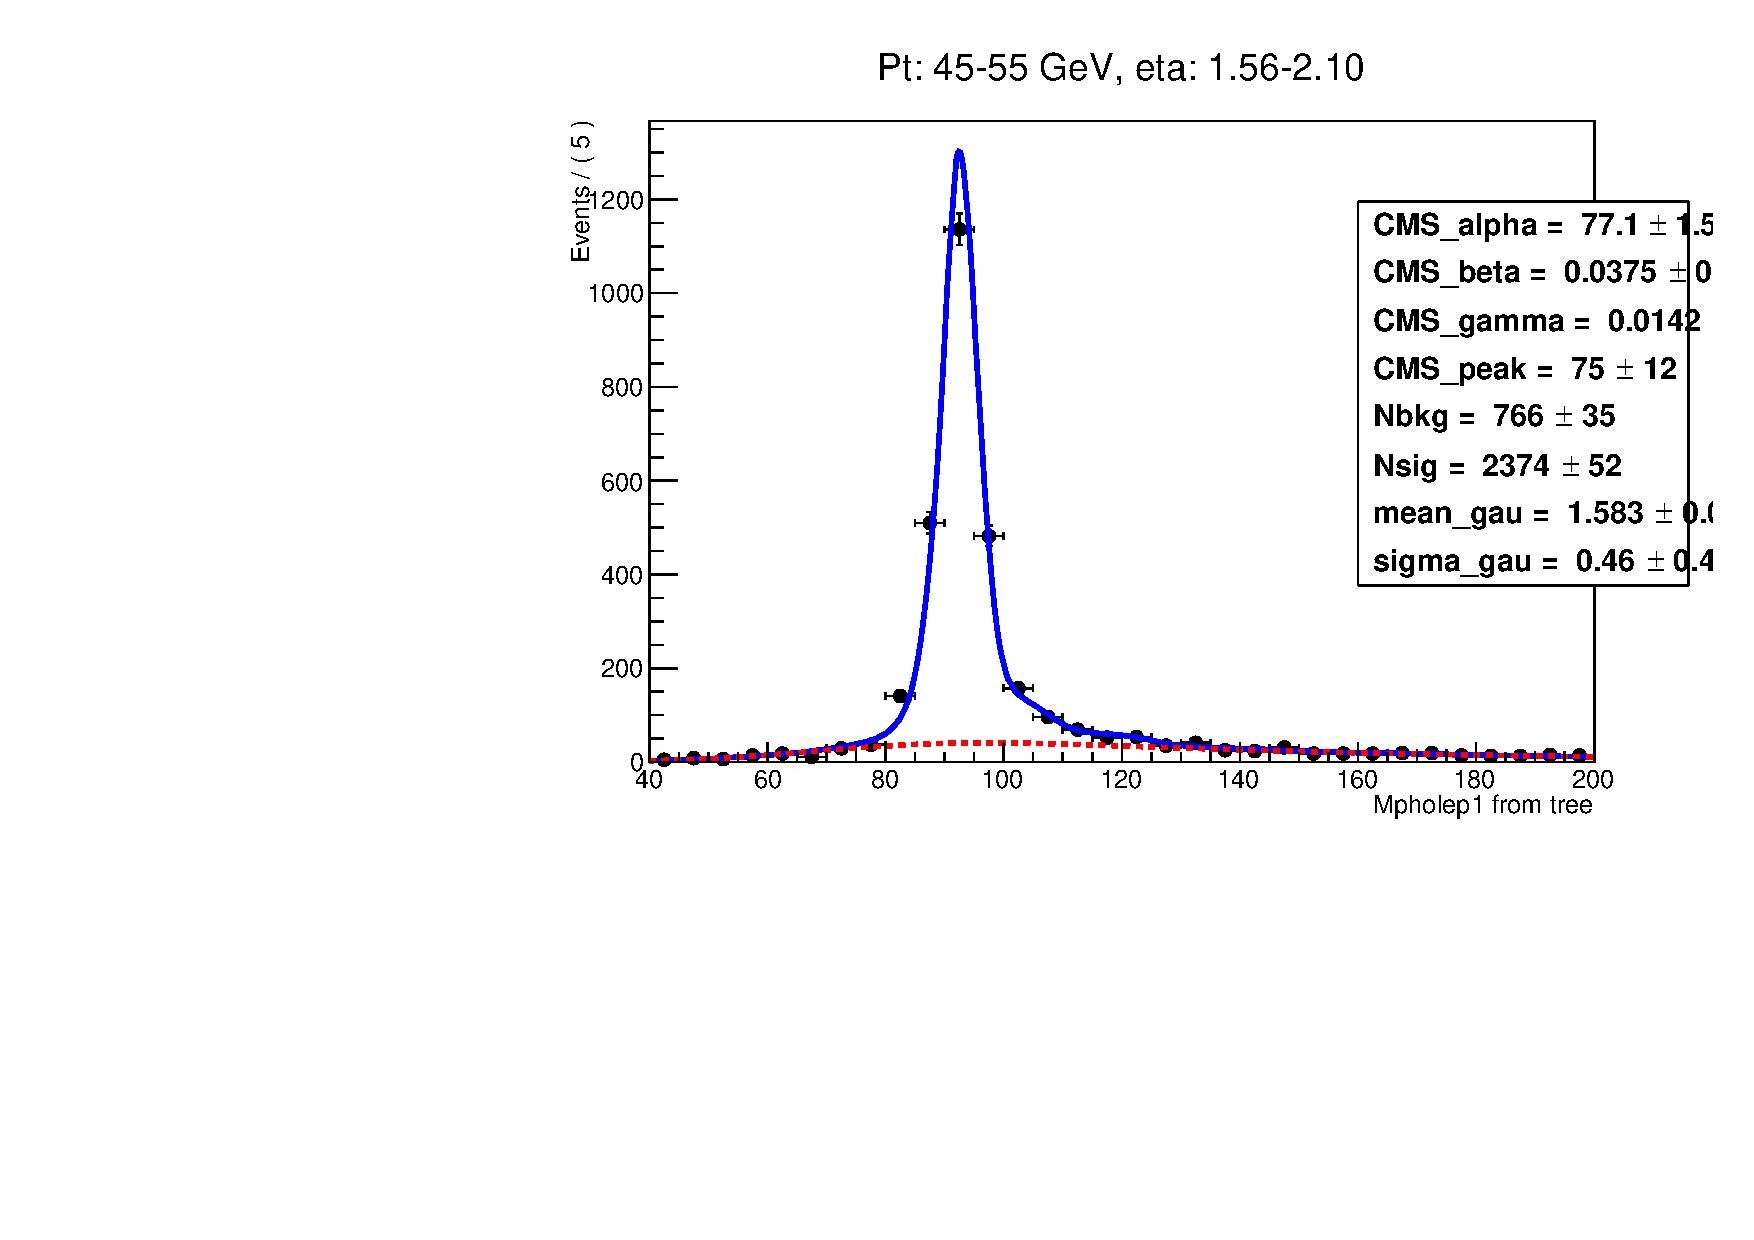
\includegraphics[width=0.45\textwidth]{../figs/figs_v11/ELECTRON_WGamma/EtoGammaFits/sa_hZmass_h_Data_EtoGamma_Enr_ENDCAP_pt45to55_ieta0.pdf}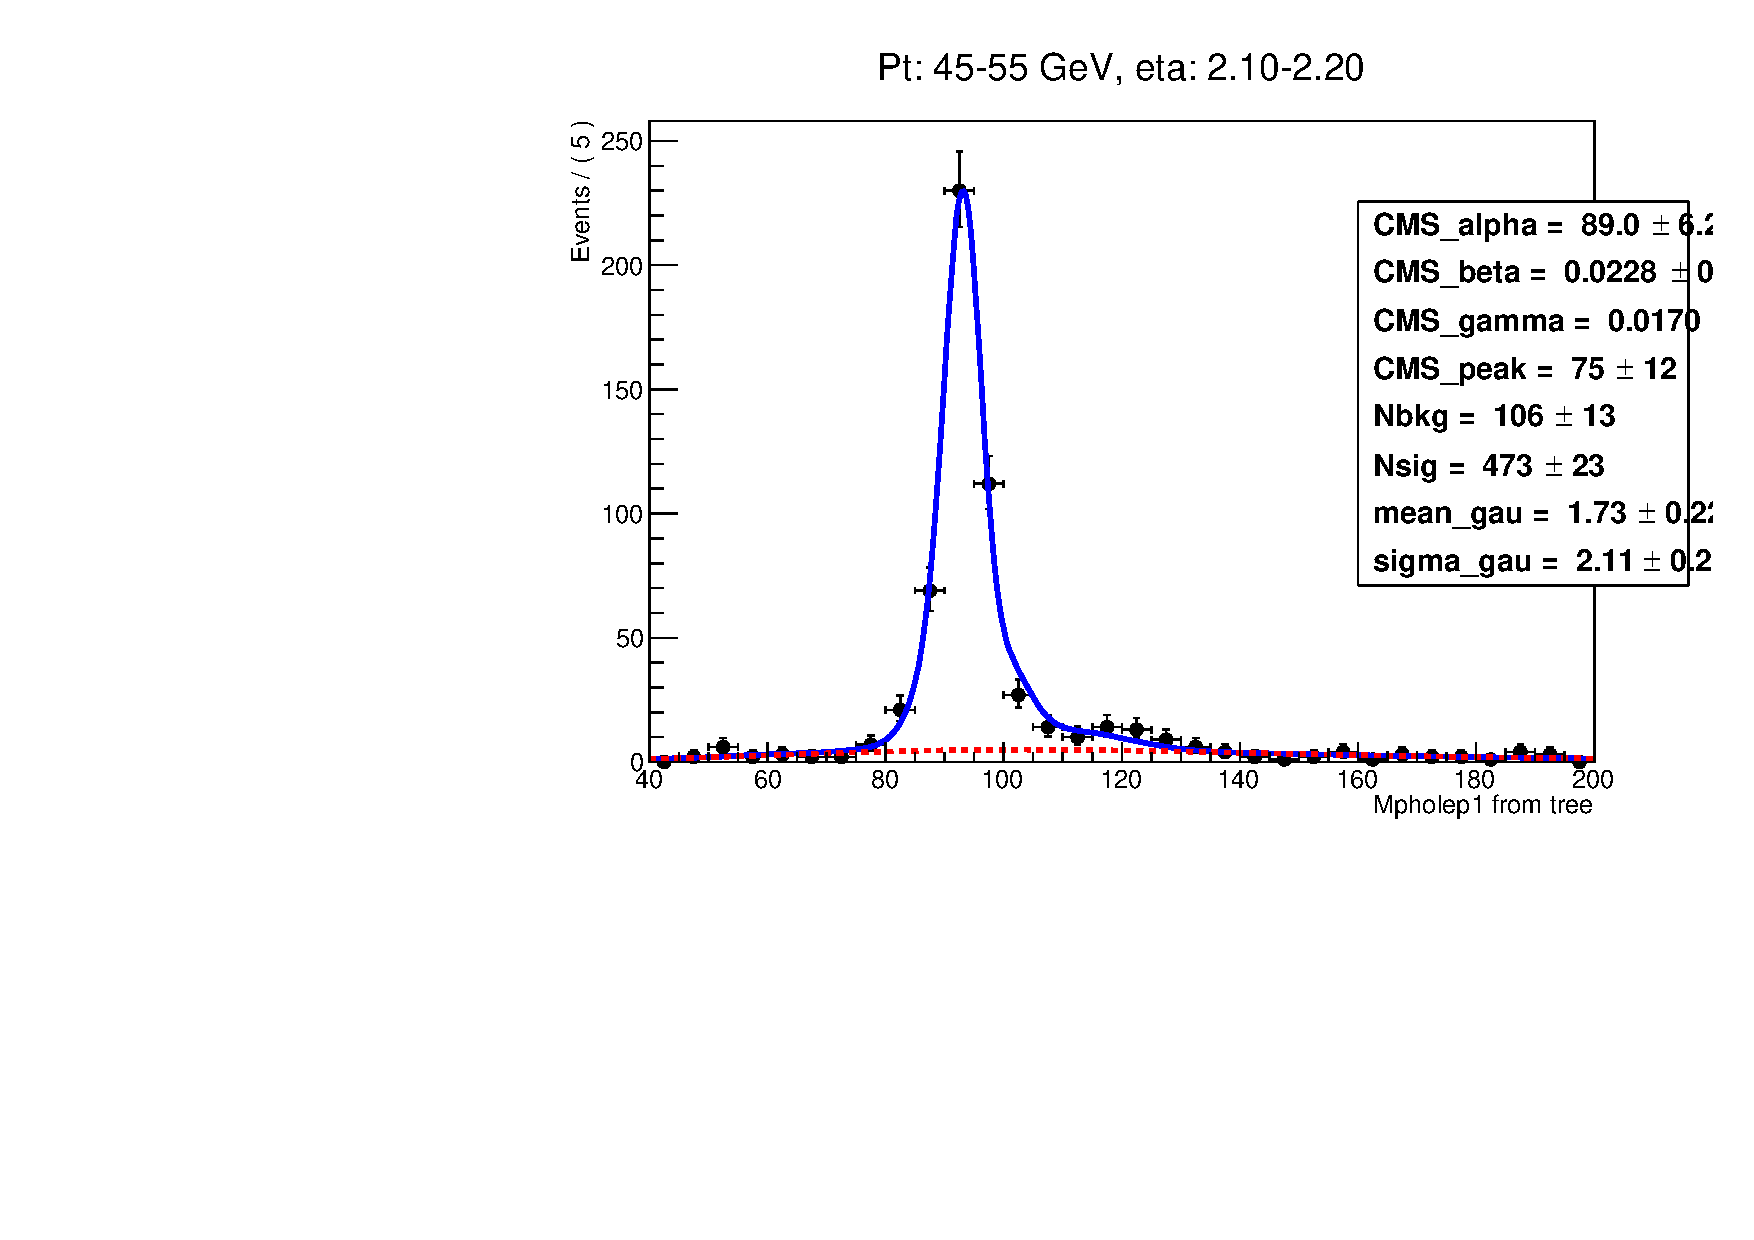
\includegraphics[width=0.45\textwidth]{../figs/figs_v11/ELECTRON_WGamma/EtoGammaFits/sa_hZmass_h_Data_EtoGamma_Enr_ENDCAP_pt45to55_ieta1.pdf}\\
   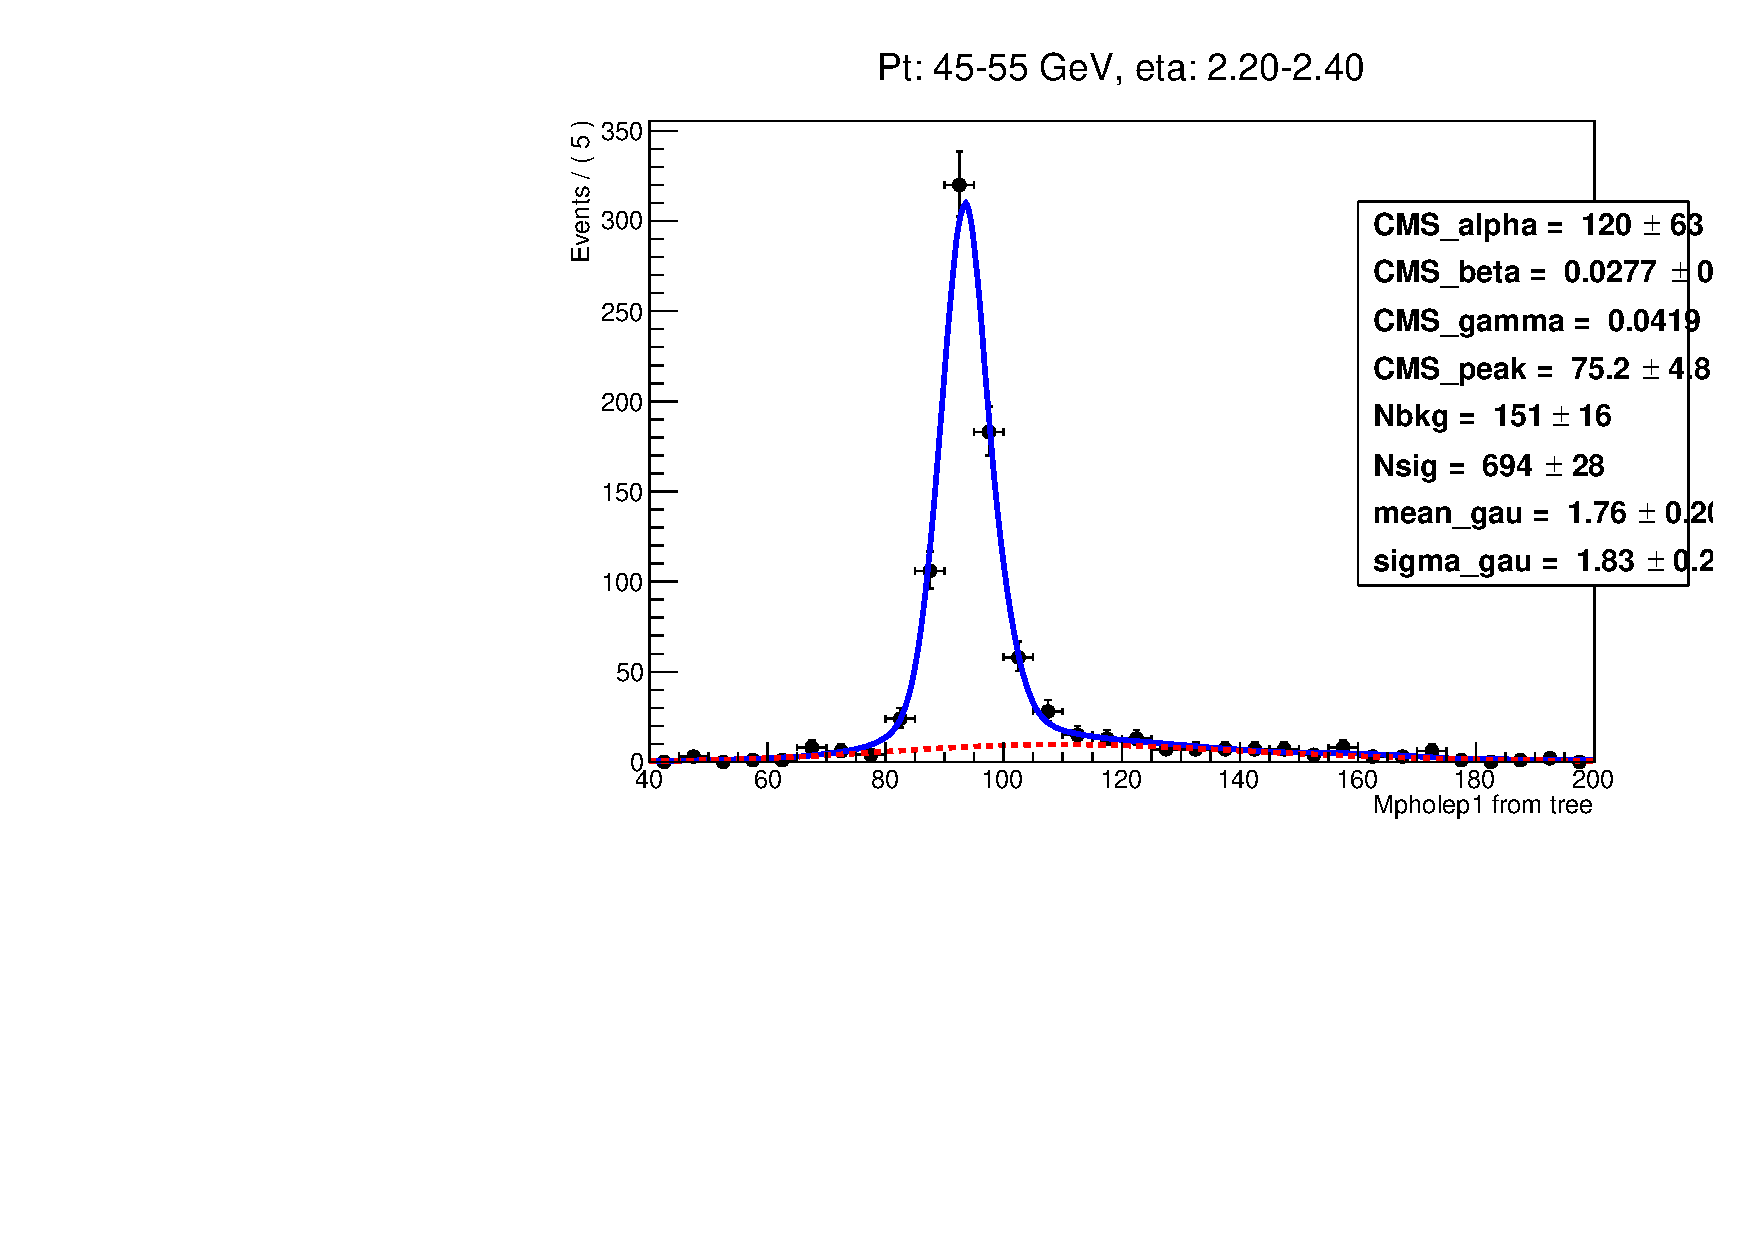
\includegraphics[width=0.45\textwidth]{../figs/figs_v11/ELECTRON_WGamma/EtoGammaFits/sa_hZmass_h_Data_EtoGamma_Enr_ENDCAP_pt45to55_ieta2.pdf}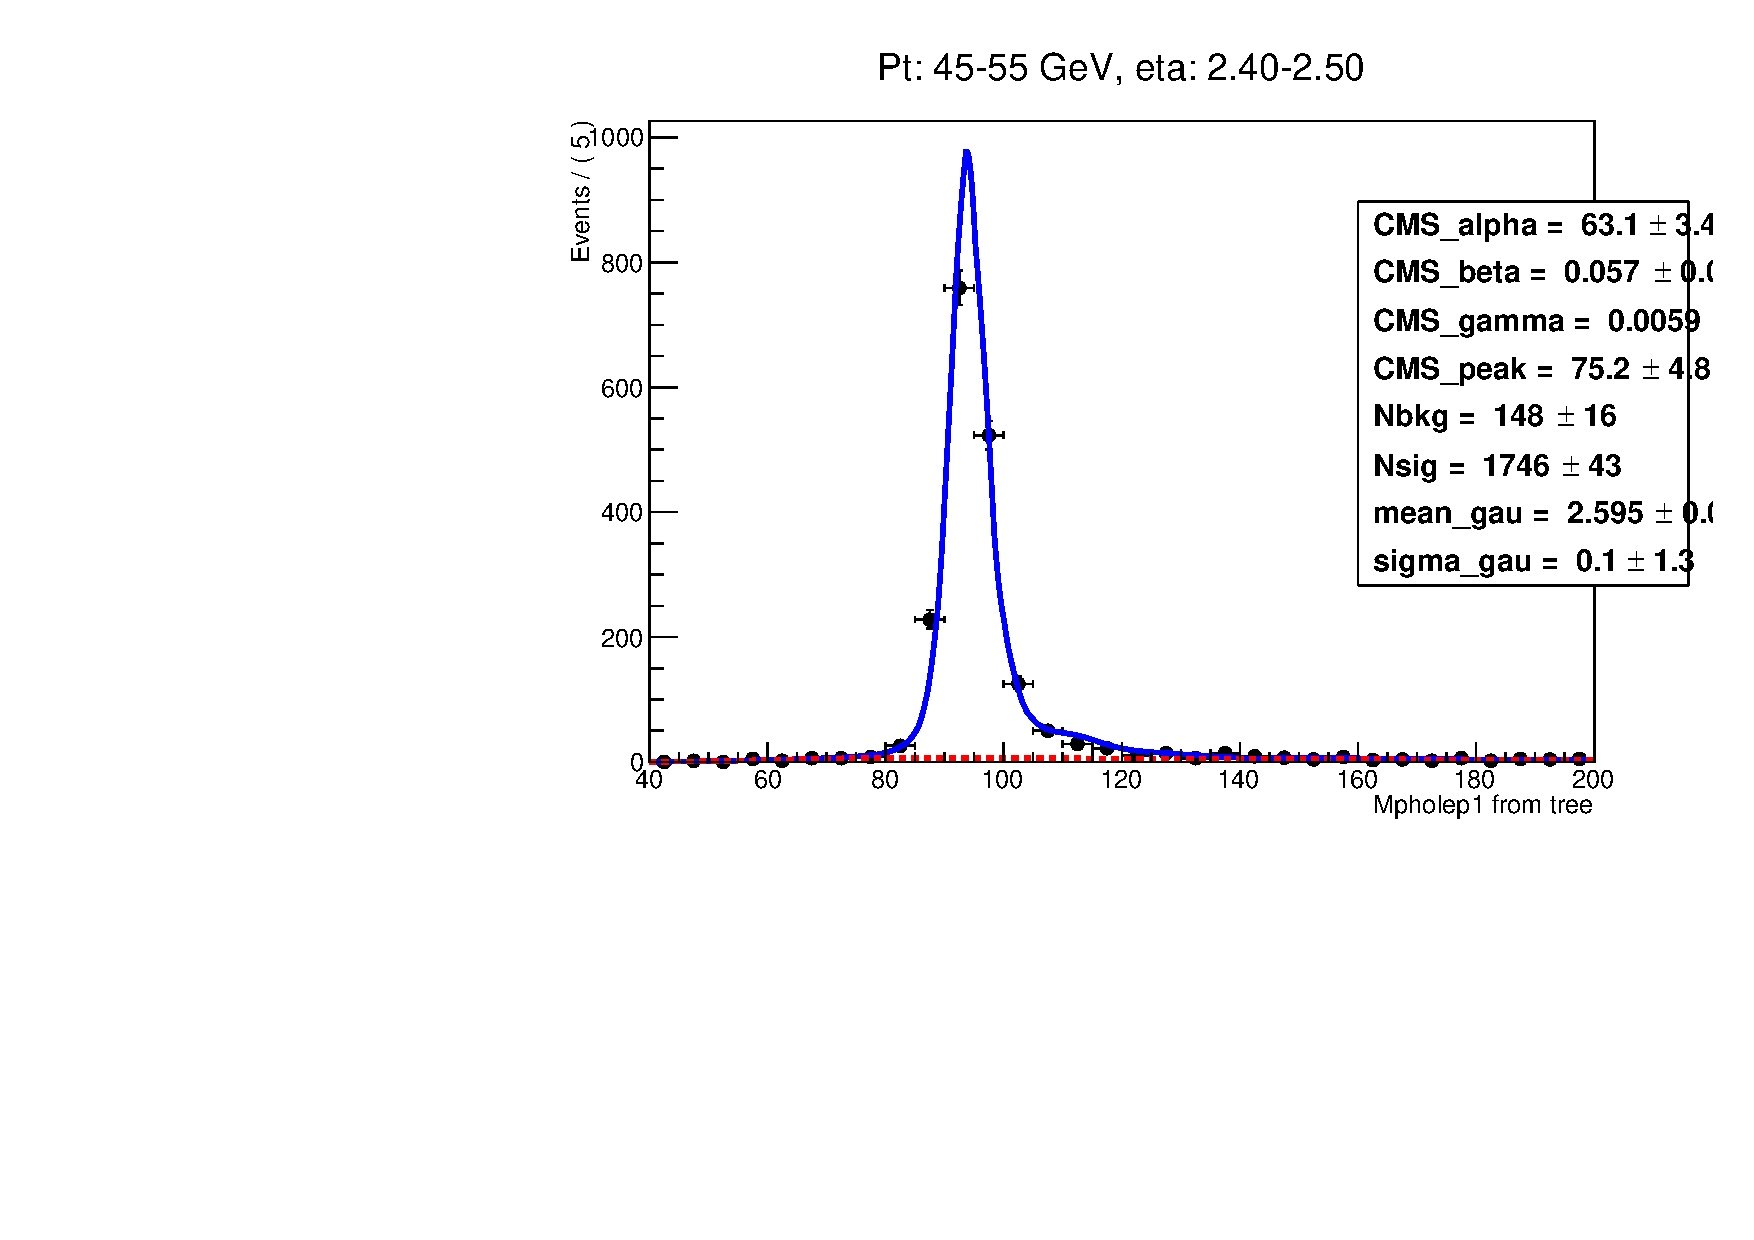
\includegraphics[width=0.45\textwidth]{../figs/figs_v11/ELECTRON_WGamma/EtoGammaFits/sa_hZmass_h_Data_EtoGamma_Enr_ENDCAP_pt45to55_ieta3.pdf}\\
  \label{fig:etogFits_45to55}
  \caption{$M_{e\gamma}$ fits, $W\gamma$, electron channel, 45-55 GeV, 8 $\eta^{\gamma}$ bins.}
  \end{center}
\end{figure}

\begin{figure}[htb]
  \begin{center}
   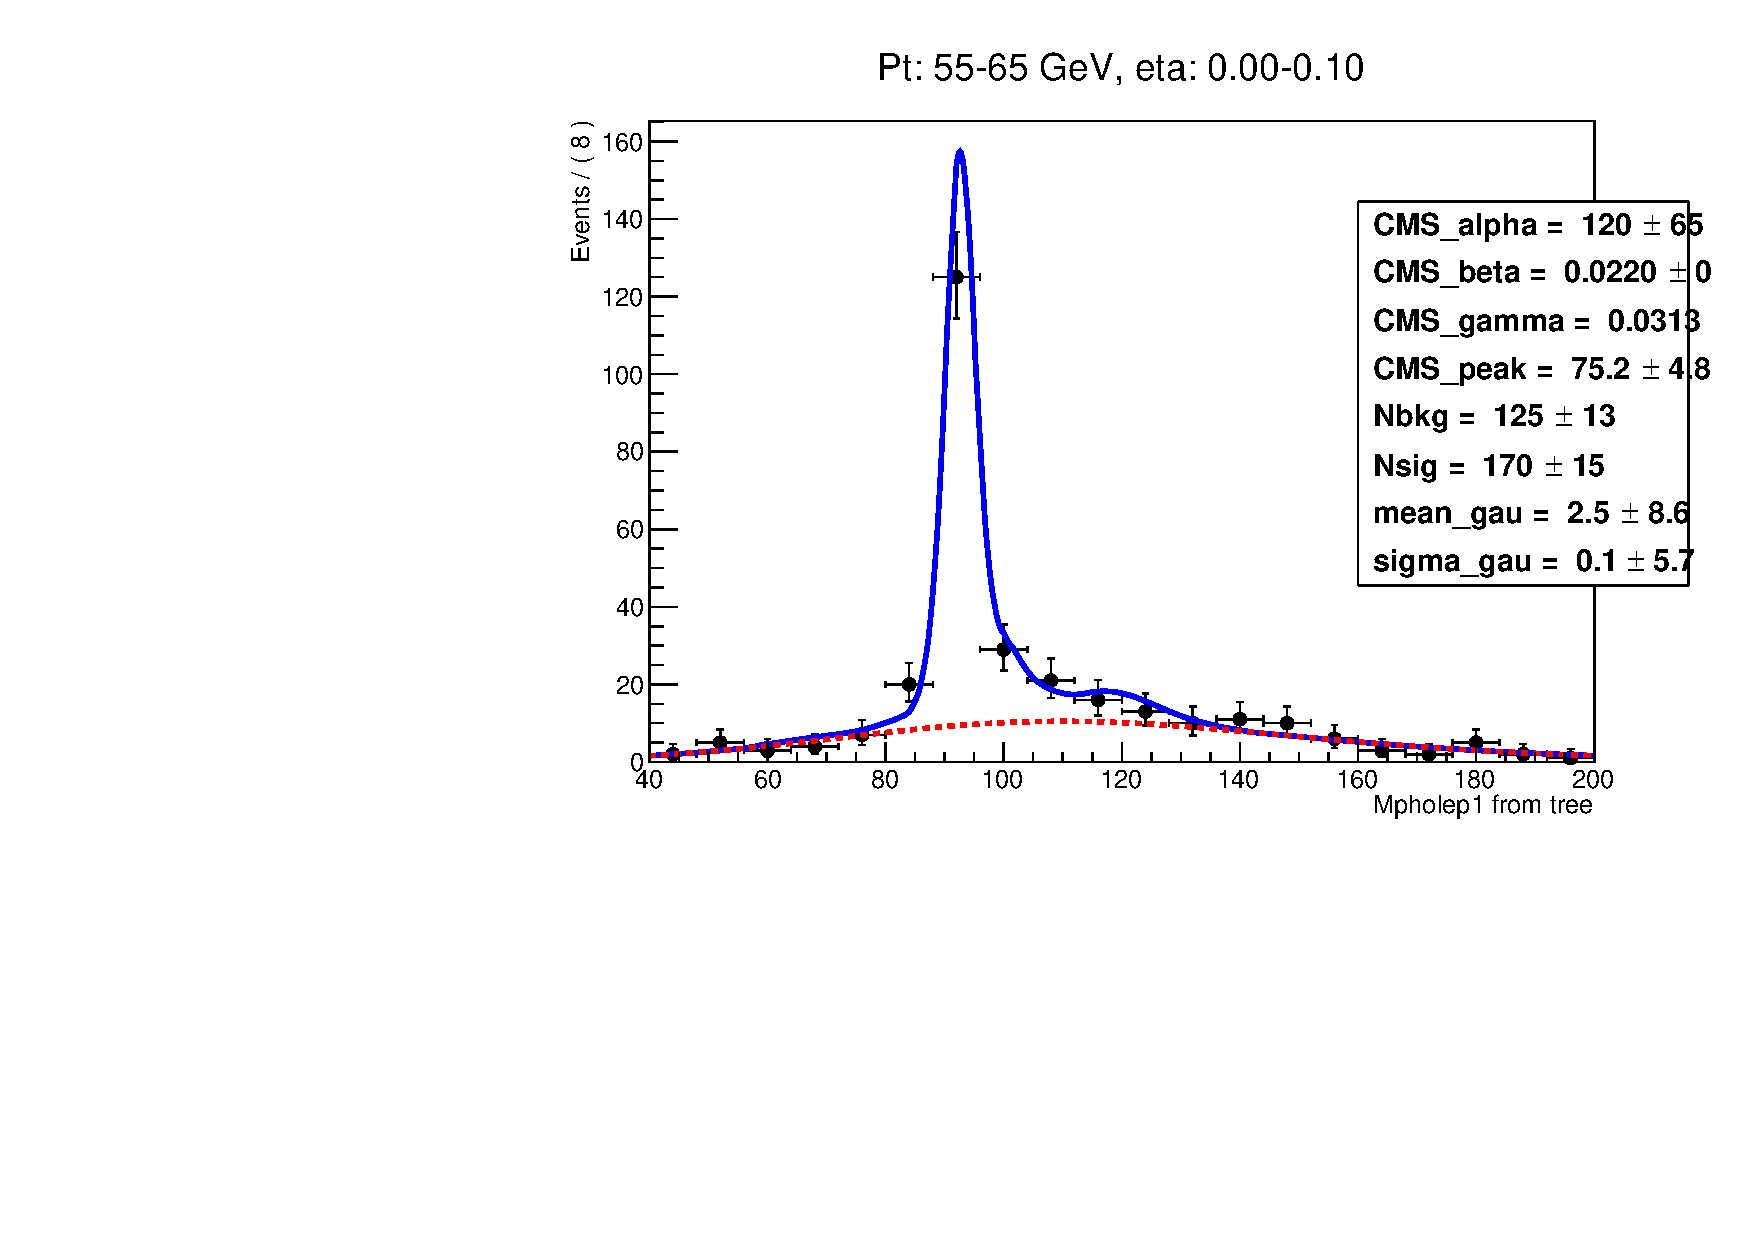
\includegraphics[width=0.45\textwidth]{../figs/figs_v11/ELECTRON_WGamma/EtoGammaFits/sa_hZmass_h_Data_EtoGamma_Enr_BARREL_pt55to65_ieta0.pdf}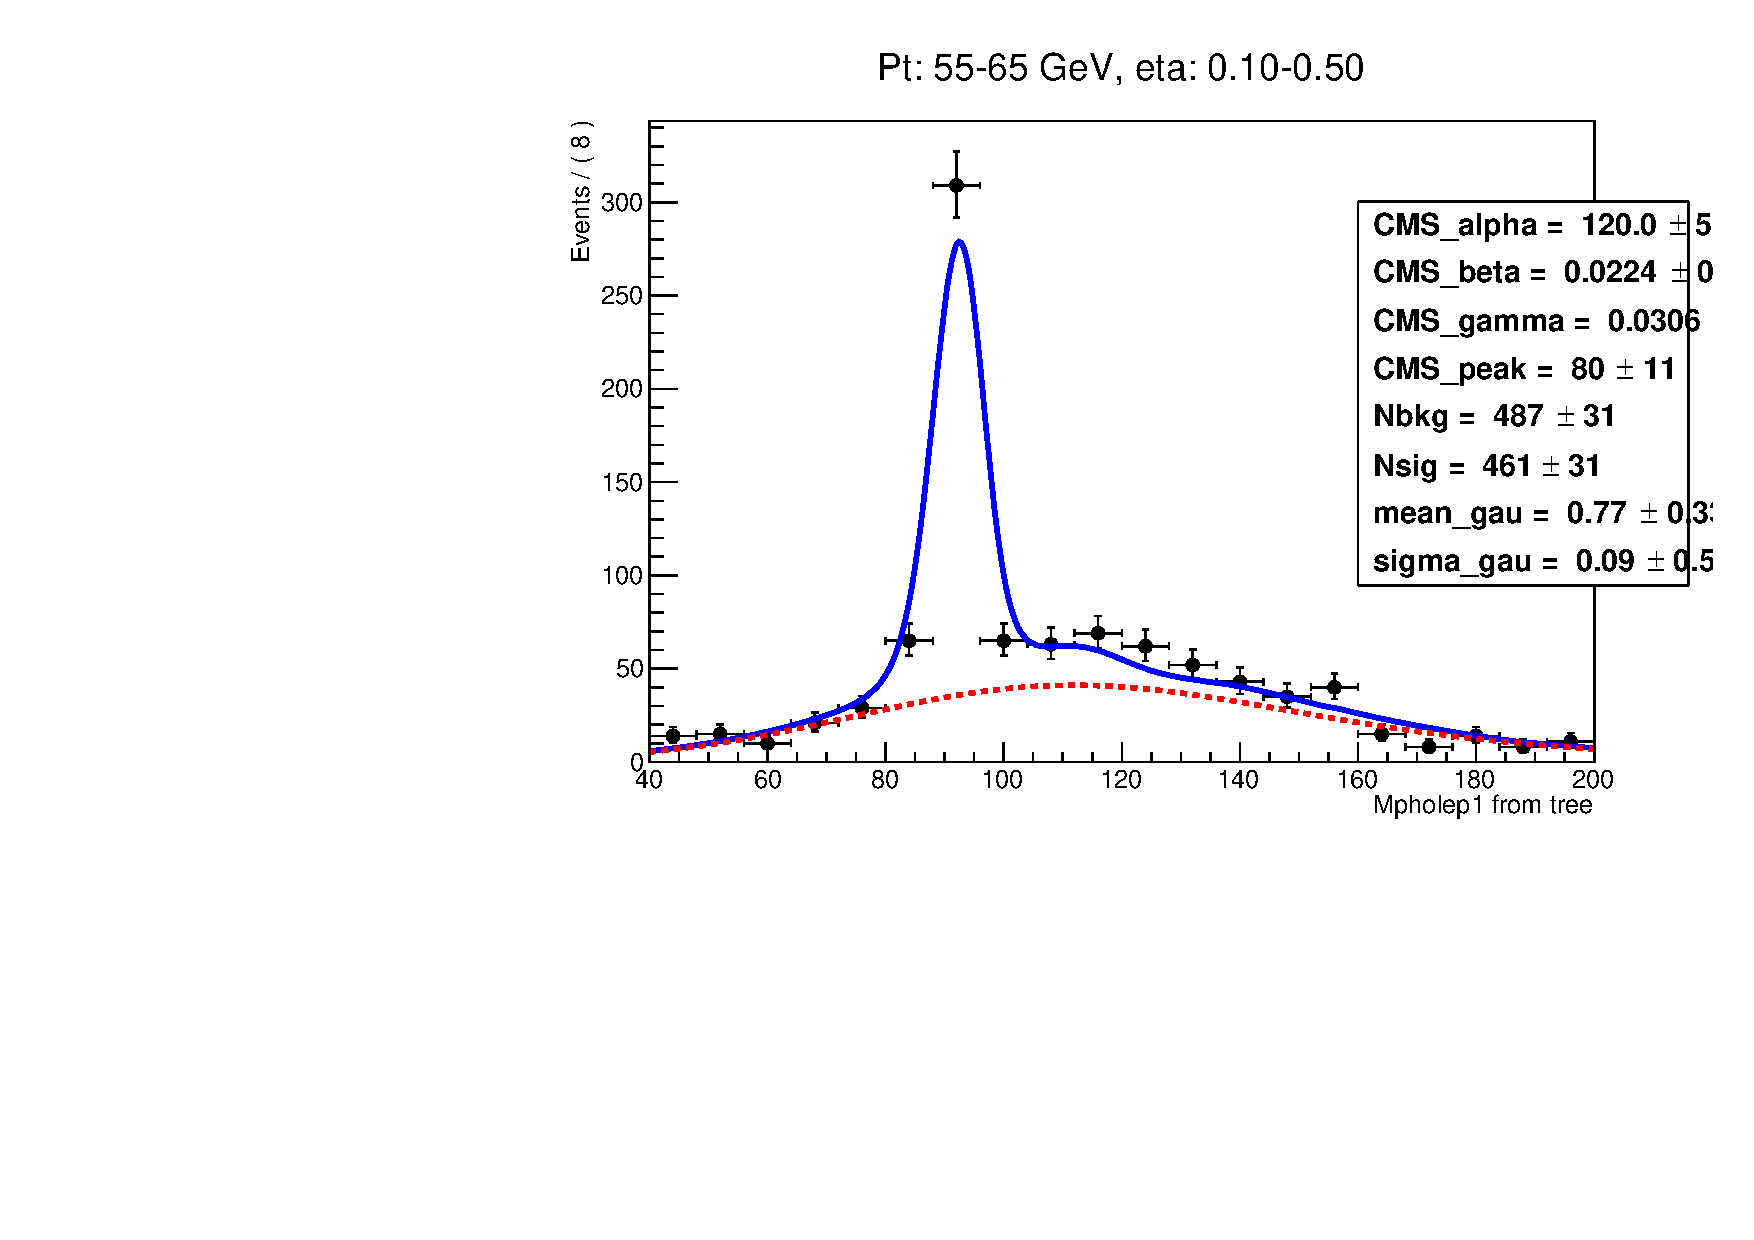
\includegraphics[width=0.45\textwidth]{../figs/figs_v11/ELECTRON_WGamma/EtoGammaFits/sa_hZmass_h_Data_EtoGamma_Enr_BARREL_pt55to65_ieta1.pdf}\\
   \includegraphics[width=0.45\textwidth]{../figs/figs_v11/ELECTRON_WGamma/EtoGammaFits/sa_hZmass_h_Data_EtoGamma_Enr_ENDCAP_pt55to65_ieta0.pdf}\includegraphics[width=0.45\textwidth]{../figs/figs_v11/ELECTRON_WGamma/EtoGammaFits/sa_hZmass_h_Data_EtoGamma_Enr_ENDCAP_pt55to65_ieta1.pdf}\\
  \label{fig:etogFits_55to65}
  \caption{$M_{e\gamma}$ fits, $W\gamma$, electron channel, 55-65 GeV, 4 $\eta^{\gamma}$ bins.}
  \end{center}
\end{figure}

\begin{figure}[htb]
  \begin{center}
   \includegraphics[width=0.45\textwidth]{../figs/figs_v11/ELECTRON_WGamma/EtoGammaFits/sa_hZmass_h_Data_EtoGamma_Enr_BARREL_pt65to75_ieta0.pdf}\includegraphics[width=0.45\textwidth]{../figs/figs_v11/ELECTRON_WGamma/EtoGammaFits/sa_hZmass_h_Data_EtoGamma_Enr_BARREL_pt65to75_ieta1.pdf}\\
   \includegraphics[width=0.45\textwidth]{../figs/figs_v11/ELECTRON_WGamma/EtoGammaFits/sa_hZmass_h_Data_EtoGamma_Enr_ENDCAP_pt65to75_ieta0.pdf}\includegraphics[width=0.45\textwidth]{../figs/figs_v11/ELECTRON_WGamma/EtoGammaFits/sa_hZmass_h_Data_EtoGamma_Enr_ENDCAP_pt65to75_ieta1.pdf}\\
  \label{fig:etogFits_65to75}
  \caption{$M_{e\gamma}$ fits, $W\gamma$, electron channel, 65-75 GeV, 4 $\eta^{\gamma}$ bins.}
  \end{center}
\end{figure}


\begin{figure}[htb]
  \begin{center}
   \includegraphics[width=0.45\textwidth]{../figs/figs_v11/ELECTRON_WGamma/EtoGammaFits/sa_hZmass_h_Data_EtoGamma_Enr_BARREL_pt75to85_ieta0.pdf}\includegraphics[width=0.45\textwidth]{../figs/figs_v11/ELECTRON_WGamma/EtoGammaFits/sa_hZmass_h_Data_EtoGamma_Enr_BARREL_pt75to85_ieta1.pdf}\\
   \includegraphics[width=0.45\textwidth]{../figs/figs_v11/ELECTRON_WGamma/EtoGammaFits/sa_hZmass_h_Data_EtoGamma_Enr_ENDCAP_pt75to85_ieta0.pdf}\includegraphics[width=0.45\textwidth]{../figs/figs_v11/ELECTRON_WGamma/EtoGammaFits/sa_hZmass_h_Data_EtoGamma_Enr_ENDCAP_pt75to85_ieta1.pdf}\\
  \label{fig:etogFits_75to85}
  \caption{$M_{e\gamma}$ fits, $W\gamma$, electron channel, 75-85 GeV, 4 $\eta^{\gamma}$ bins.}
  \end{center}
\end{figure}

\begin{figure}[htb]
  \begin{center}
   \includegraphics[width=0.45\textwidth]{../figs/figs_v11/ELECTRON_WGamma/EtoGammaFits/sa_hZmass_h_Data_EtoGamma_Enr_BARREL_pt85to95_ieta0.pdf}
   \includegraphics[width=0.45\textwidth]{../figs/figs_v11/ELECTRON_WGamma/EtoGammaFits/sa_hZmass_h_Data_EtoGamma_Enr_ENDCAP_pt85to95_ieta0.pdf}\\
  \label{fig:etogFits_85to95}
  \caption{$M_{e\gamma}$ fits, $W\gamma$, electron channel, 85-95 GeV, 2 $\eta^{\gamma}$ bins.}
  \end{center}
\end{figure}

\begin{figure}[htb]
  \begin{center}
   \includegraphics[width=0.45\textwidth]{../figs/figs_v11/ELECTRON_WGamma/EtoGammaFits/sa_hZmass_h_Data_EtoGamma_Enr_BARREL_pt95to120_ieta0.pdf}
   \includegraphics[width=0.45\textwidth]{../figs/figs_v11/ELECTRON_WGamma/EtoGammaFits/sa_hZmass_h_Data_EtoGamma_Enr_ENDCAP_pt95to120_ieta0.pdf}\\
  \label{fig:etogFits_95to120}
  \caption{$M_{e\gamma}$ fits, $W\gamma$, electron channel, 95-120 GeV, 2 $\eta^{\gamma}$ bins.}
  \end{center}
\end{figure}

\begin{figure}[htb]
  \begin{center}
   \includegraphics[width=0.45\textwidth]{../figs/figs_v11/ELECTRON_WGamma/EtoGammaFits/sa_hZmass_h_Data_EtoGamma_Enr_BARREL_pt120to500_ieta0.pdf}
   \includegraphics[width=0.45\textwidth]{../figs/figs_v11/ELECTRON_WGamma/EtoGammaFits/sa_hZmass_h_Data_EtoGamma_Enr_ENDCAP_pt120to500_ieta0.pdf}\\
  \label{fig:etogFits_120to500}
  \caption{$M_{e\gamma}$ fits, $W\gamma$, electron channel, 120-500 GeV, 2 $\eta^{\gamma}$ bins.}
  \end{center}
\end{figure}


